%%%%%%%%%%%%%%%%%%%%%%%%%%%%%%%%%%%%%%%%%
% Cleese Assignment (For Students)
% LaTeX Template
% Version 2.0 (27/5/2018)
%
% This template originates from:
% http://www.LaTeXTemplates.com
%
% Author:
% Vel (vel@LaTeXTemplates.com)
%
% License:
% CC BY-NC-SA 3.0 (http://creativecommons.org/licenses/by-nc-sa/3.0/)
% 
%%%%%%%%%%%%%%%%%%%%%%%%%%%%%%%%%%%%%%%%%

%----------------------------------------------------------------------------------------
%	PACKAGES AND OTHER DOCUMENT CONFIGURATIONS
%----------------------------------------------------------------------------------------

\documentclass[11pt]{article}
\usepackage{float}

%\usepackage[printwatermark]{xwatermark}
%\newwatermark[allpages,color=gray!50,angle=45,scale=2.5,xpos=-5,ypos=-5]{Mohammad Hadi}

%%%%%%%%%%%%%%%%%%%%%%%%%%%%%%%%%%%%%%%%%
% Cleese Assignment
% Structure Specification File
% Version 1.0 (27/5/2018)
%
% This template originates from:
% http://www.LaTeXTemplates.com
%
% Author:
% Vel (vel@LaTeXTemplates.com)
%
% License:
% CC BY-NC-SA 3.0 (http://creativecommons.org/licenses/by-nc-sa/3.0/)
% 
%%%%%%%%%%%%%%%%%%%%%%%%%%%%%%%%%%%%%%%%%

%----------------------------------------------------------------------------------------
%	PACKAGES AND OTHER DOCUMENT CONFIGURATIONS
%----------------------------------------------------------------------------------------

\usepackage{lastpage} % Required to determine the last page number for the footer

\usepackage{graphicx} % Required to insert images

\setlength\parindent{0pt} % Removes all indentation from paragraphs

\usepackage[most]{tcolorbox} % Required for boxes that split across pages

\usepackage{booktabs} % Required for better horizontal rules in tables

\usepackage{listings} % Required for insertion of code

\usepackage{etoolbox} % Required for if statements

%----------------------------------------------------------------------------------------
%	MARGINS
%----------------------------------------------------------------------------------------

\usepackage{geometry} % Required for adjusting page dimensions and margins

\geometry{
	paper=a4paper, % Change to letterpaper for US letter
	top=3cm, % Top margin
	bottom=3cm, % Bottom margin
	left=2.5cm, % Left margin
	right=2.5cm, % Right margin
	headheight=14pt, % Header height
	footskip=1.4cm, % Space from the bottom margin to the baseline of the footer
	headsep=1.2cm, % Space from the top margin to the baseline of the header
	%showframe, % Uncomment to show how the type block is set on the page
}

%----------------------------------------------------------------------------------------
%	FONT
%----------------------------------------------------------------------------------------

\usepackage[utf8]{inputenc} % Required for inputting international characters
\usepackage[T1]{fontenc} % Output font encoding for international characters

\usepackage[sfdefault,light]{roboto} % Use the Roboto font

%----------------------------------------------------------------------------------------
%	HEADERS AND FOOTERS
%----------------------------------------------------------------------------------------

\usepackage{fancyhdr} % Required for customising headers and footers

\pagestyle{fancy} % Enable custom headers and footers

\lhead{\small\assignmentClass\ifdef{\assignmentClassInstructor}{\ (\assignmentClassInstructor):}{}\ \assignmentTitle} % Left header; output the instructor in brackets if one was set
\chead{} % Centre header
\rhead{\small\ifdef{\assignmentAuthorName}{\assignmentAuthorName}{\ifdef{\assignmentDueDate}{Due\ \assignmentDueDate}{}}} % Right header; output the author name if one was set, otherwise the due date if that was set

\lfoot{} % Left footer
\cfoot{\small Page\ \thepage\ of\ \pageref{LastPage}} % Centre footer
\rfoot{} % Right footer

\renewcommand\headrulewidth{0.5pt} % Thickness of the header rule

%----------------------------------------------------------------------------------------
%	MODIFY SECTION STYLES
%----------------------------------------------------------------------------------------

\usepackage{titlesec} % Required for modifying sections

%------------------------------------------------
% Section

\titleformat
{\section} % Section type being modified
[block] % Shape type, can be: hang, block, display, runin, leftmargin, rightmargin, drop, wrap, frame
{\Large\bfseries} % Format of the whole section
{\assignmentQuestionName~\thesection} % Format of the section label
{6pt} % Space between the title and label
{} % Code before the label

\titlespacing{\section}{0pt}{0.5\baselineskip}{0.5\baselineskip} % Spacing around section titles, the order is: left, before and after

%------------------------------------------------
% Subsection

\titleformat
{\subsection} % Section type being modified
[block] % Shape type, can be: hang, block, display, runin, leftmargin, rightmargin, drop, wrap, frame
{\itshape} % Format of the whole section
{(\alph{subsection})} % Format of the section label
{4pt} % Space between the title and label
{} % Code before the label

\titlespacing{\subsection}{0pt}{0.5\baselineskip}{0.5\baselineskip} % Spacing around section titles, the order is: left, before and after

\renewcommand\thesubsection{(\alph{subsection})}

%----------------------------------------------------------------------------------------
%	CUSTOM QUESTION COMMANDS/ENVIRONMENTS
%----------------------------------------------------------------------------------------

% Environment to be used for each question in the assignment
\newenvironment{question}{
	\vspace{0.5\baselineskip} % Whitespace before the question
	\section{} % Blank section title (e.g. just Question 2)
	\lfoot{\small\itshape\assignmentQuestionName~\thesection~continued on next page\ldots} % Set the left footer to state the question continues on the next page, this is reset to nothing if it doesn't (below)
}{
	\lfoot{} % Reset the left footer to nothing if the current question does not continue on the next page
}

%------------------------------------------------

% Environment for subquestions, takes 1 argument - the name of the section
\newenvironment{subquestion}[1]{
	\subsection{#1}
}{
}

%------------------------------------------------

% Command to print a question sentence
\newcommand{\questiontext}[1]{
	\textbf{#1}
	\vspace{0.5\baselineskip} % Whitespace afterwards
}

%------------------------------------------------

% Command to print a box that breaks across pages with the question answer
\newcommand{\answer}[1]{
	\begin{tcolorbox}[breakable, enhanced]
		#1
	\end{tcolorbox}
}

%------------------------------------------------

% Command to print a box that breaks across pages with the space for a student to answer
\newcommand{\answerbox}[1]{
	\begin{tcolorbox}[breakable, enhanced]
		\vphantom{L}\vspace{\numexpr #1-1\relax\baselineskip} % \vphantom{L} to provide a typesetting strut with a height for the line, \numexpr to subtract user input by 1 to make it 0-based as this command is
	\end{tcolorbox}
}

%------------------------------------------------

% Command to print an assignment section title to split an assignment into major parts
\newcommand{\assignmentSection}[1]{
	{
		\centering % Centre the section title
		\vspace{2\baselineskip} % Whitespace before the entire section title
		
		\rule{0.8\textwidth}{0.5pt} % Horizontal rule
		
		\vspace{0.75\baselineskip} % Whitespace before the section title
		{\LARGE \MakeUppercase{#1}} % Section title, forced to be uppercase
		
		\rule{0.8\textwidth}{0.5pt} % Horizontal rule
		
		\vspace{\baselineskip} % Whitespace after the entire section title
	}
}

%----------------------------------------------------------------------------------------
%	TITLE PAGE
%----------------------------------------------------------------------------------------

\author{\textbf{\assignmentAuthorName}} % Set the default title page author field
\date{} % Don't use the default title page date field

\title{
	\thispagestyle{empty} % Suppress headers and footers
	\vspace{0.2\textheight} % Whitespace before the title
	\textbf{\assignmentClass:\ \assignmentTitle}\\[-4pt]
	\ifdef{\assignmentDueDate}{{\small Due\ on\ \assignmentDueDate}\\}{} % If a due date is supplied, output it
	\ifdef{\assignmentClassInstructor}{{\large \textit{\assignmentClassInstructor}}}{} % If an instructor is supplied, output it
	\vspace{0.32\textheight} % Whitespace before the author name
}
 % Include the file specifying the document structure and custom commands

%----------------------------------------------------------------------------------------
%	ASSIGNMENT INFORMATION
%----------------------------------------------------------------------------------------

% Required
\newcommand{\assignmentQuestionName}{Experiment} % The word to be used as a prefix to question numbers; example alternatives: Problem, Exercise
\newcommand{\assignmentClass}{Electrical Circuits Lab (Taught by Mohammad Hadi)\\Manual 7 (Due on DDD.,\ mmm.\ dd,\ yyyy)} % Course (Lecturer)\\Assignment (Due date)
\newcommand{\assignmentTitle}{} % Assignment title or name
\newcommand{\assignmentAuthorName}{Sina Hashemi \& M.Mahdi Shokrzade\\402102668 - 402101985} % Student name\\Student number
%----------------------------------------------------------------------------------------
\newcommand{\PicScale}{0.2}

\begin{document}
\textbf{Frequency response is a measurable concept that can be used to experimentally and analytically describe a circuit. In this experiment, you become familiar with the frequency response of first- and second-order circuits.
}
%----------------------------------------------------------------------------------------
%	TITLE PAGE
%----------------------------------------------------------------------------------------

\assignmentSection{Mandatory Experiments}

%----------------------------------------------------------------------------------------
%	QUESTION 1
%----------------------------------------------------------------------------------------

\begin{question}

    \questiontext{Build the circuit shown in Fig. \ref{fig:cir1} on a breadboard. Instead of using a physical switch, connect or disconnect the supply wire.}

    \begin{figure}[H]
        \centering
        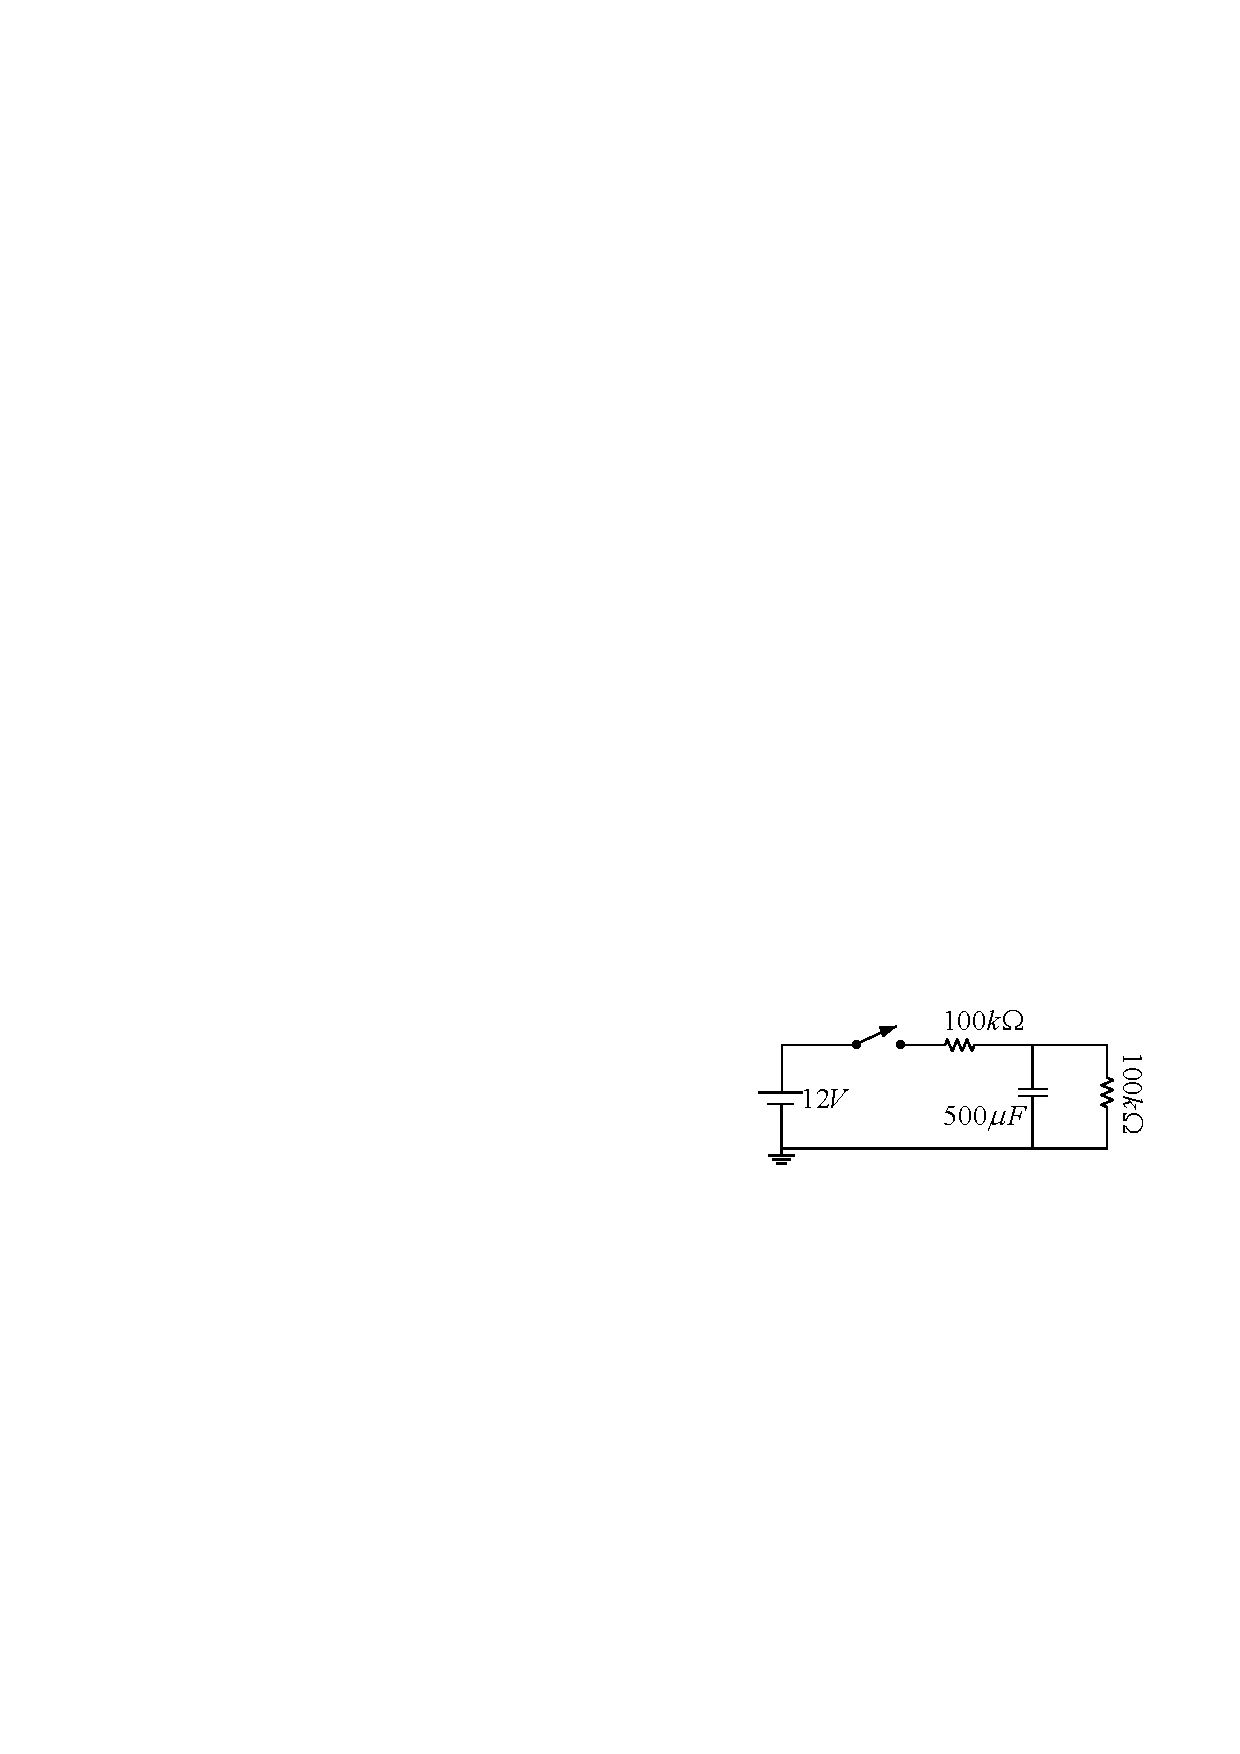
\includegraphics[scale=1.2,angle=0]{Fig/cir1.pdf}
        \caption{An RC circuit.} \label{fig:cir1}
    \end{figure}

    %--------------------------------------------
    \begin{subquestion}{Connect and disconnect the supplu wire to see the capacitor voltage response on the oscilloscope screen. Discuss the results.}
        \answer{
            \begin{figure}[H]
                \centering
                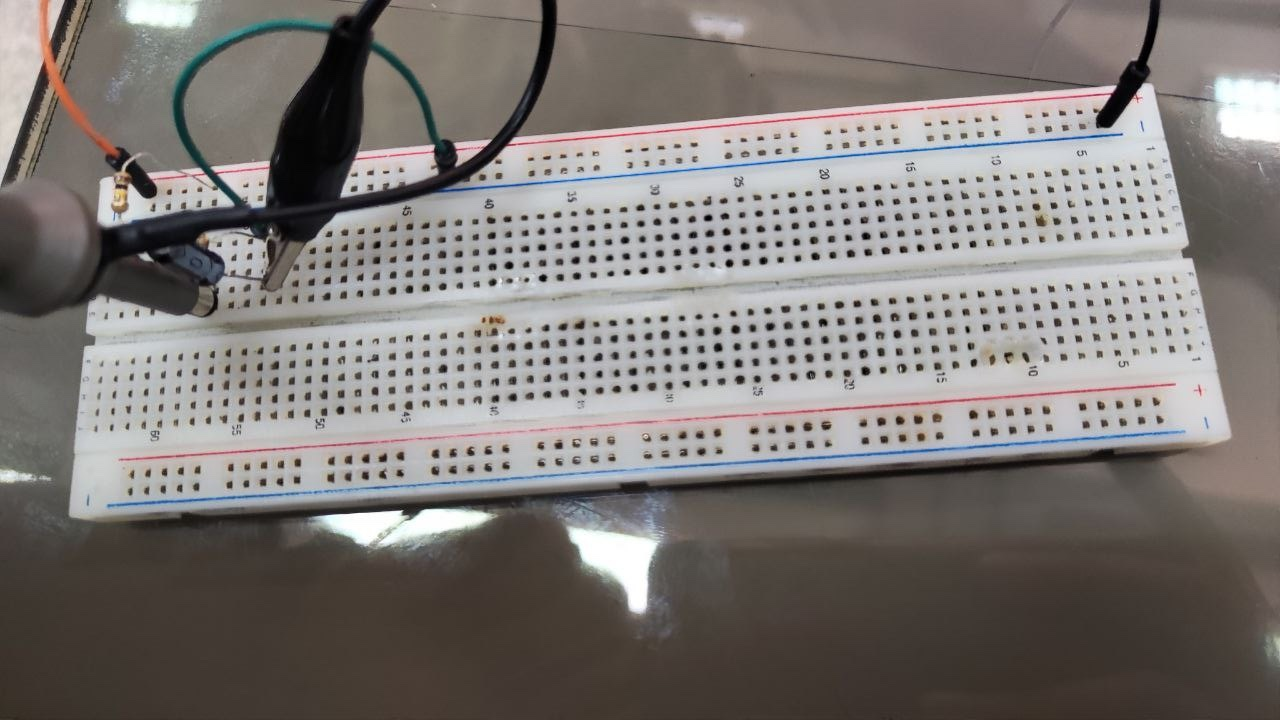
\includegraphics[scale=\PicScale,angle=0]{Fig/1.jpeg}
                \caption{The circuit.}
            \end{figure}
            \begin{figure}[H]
                \centering
                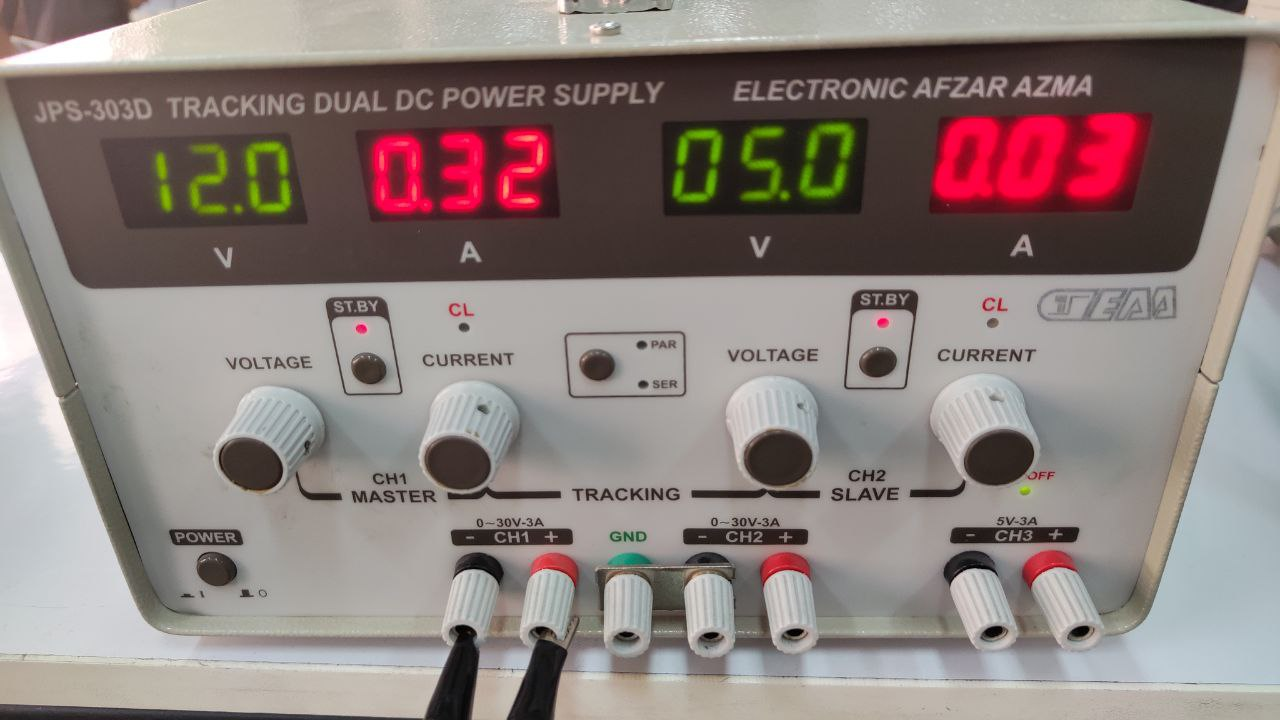
\includegraphics[scale=\PicScale,angle=0]{Fig/2.jpeg}
                \caption{The DC power supply setup.}
            \end{figure}
            \begin{figure}[H]
                \centering
                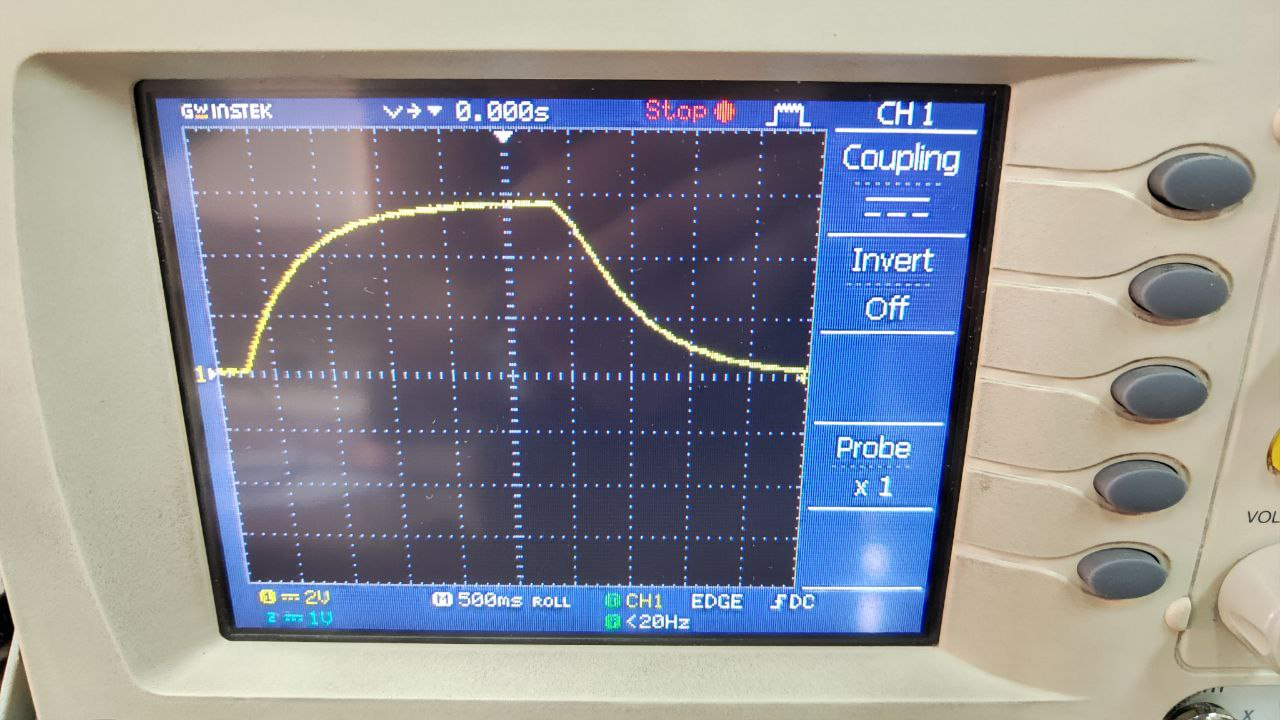
\includegraphics[scale=\PicScale,angle=0]{Fig/3.jpeg}
                \caption{The capacitor charge and discharge on oscilloscope's screen.}
            \end{figure}
            As you can see, by connecting the current, the capacitor is charged and when the current is cut off, the capacitor is discharged.
        }
    \end{subquestion}

    %--------------------------------------------
    \begin{subquestion}{Measure the time constant of the circuit and compare it to its analytical counterpart.}
        \answer{
            The time required to reach approximately $63\%$ of the maximum capacitor voltage is one $\tau$. So $\tau \cong 400m$. \\
            If we calculate the time constant using analytical methods, we need to calculate $R_{eq}C$. So:
            \[
                \tau_{analytical} = R_{eq}C = 50k \cdot 10\mu = 500m
            \]
            As expected, The two analytical and practical values are close.
        }
    \end{subquestion}

    %--------------------------------------------
    \begin{subquestion}{Decrease the supply voltage to $5$ V and redo the previous parts.}
        \answer{
            \begin{figure}[H]
                \centering
                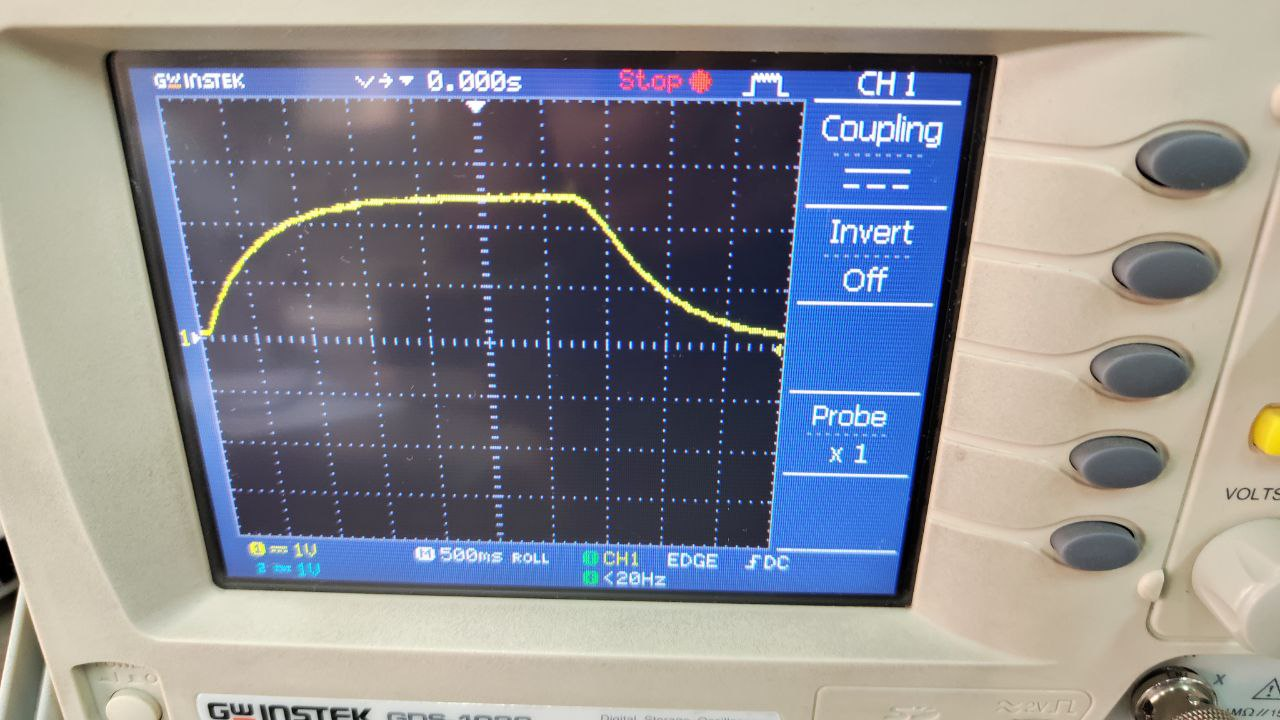
\includegraphics[scale=\PicScale,angle=0]{Fig/4.jpeg}
                \caption{The capacitor charge and discharge on oscilloscope's screen.}
            \end{figure}
            The time required to reach approximately $63\%$ of the maximum capacitor voltage is one $\tau$. So $\tau \cong 500m$. \\
            If we compare this number to $\tau_{analytical}$, the analytical value and the practical value are the same. \\
            As we expected, the time constant is independent of the voltage.
        }
    \end{subquestion}


\end{question}

%----------------------------------------------------------------------------------------
%	QUESTION 2
%----------------------------------------------------------------------------------------

\begin{question}

    \questiontext{Build the circuit shown in Fig. \ref{fig:cir2} on a breadboard.}

    \begin{figure}[H]
        \centering
        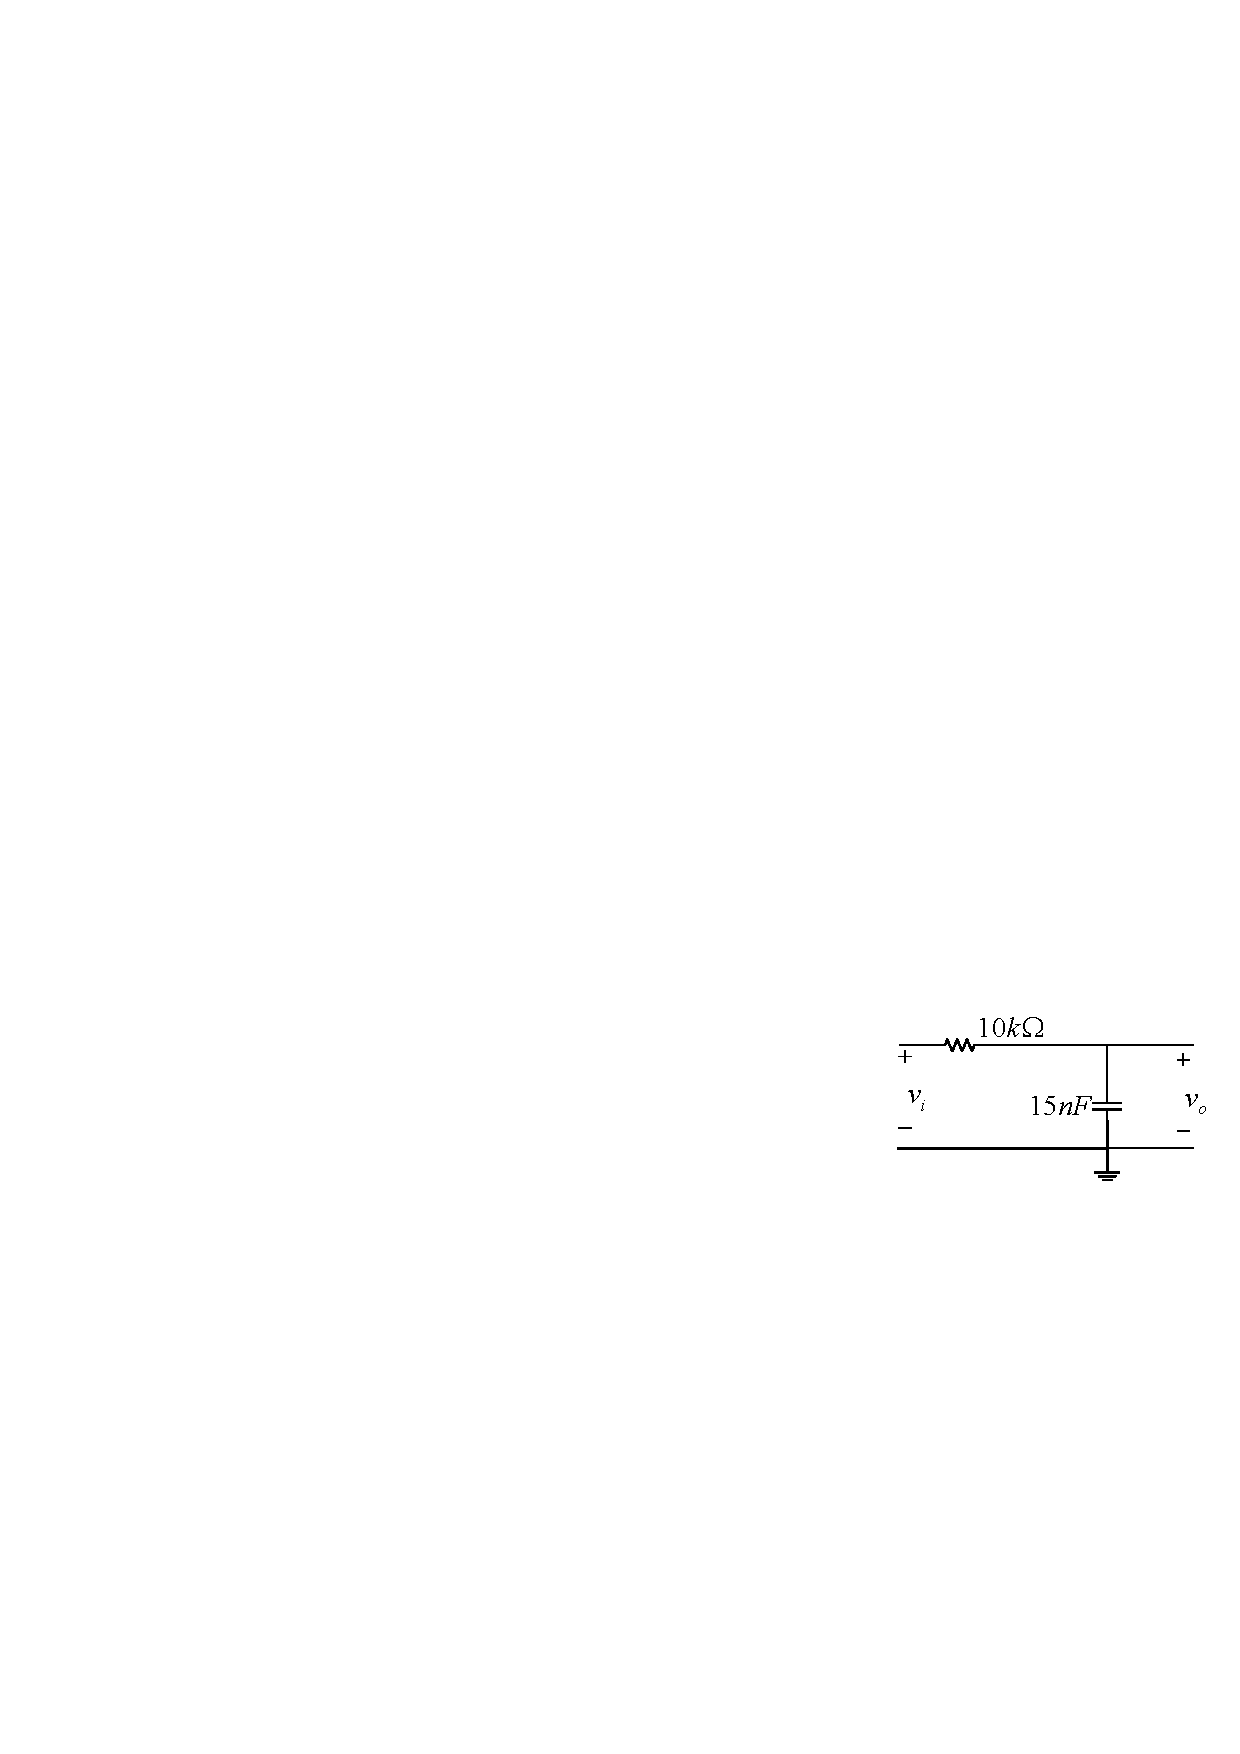
\includegraphics[scale=1.2,angle=0]{Fig/cir2.pdf}
        \caption{A lowpass RC circuit.} \label{fig:cir2}
    \end{figure}

    %--------------------------------------------
    \begin{subquestion}{Apply a $1$-V $300$-Hz square wave to the input. See the input and output voltages simultaneously on the oscilloscope screen. Interpret the observations. Obtain the time constant of the circuit.}
        \answer{
            \begin{figure}[H]
                \centering
                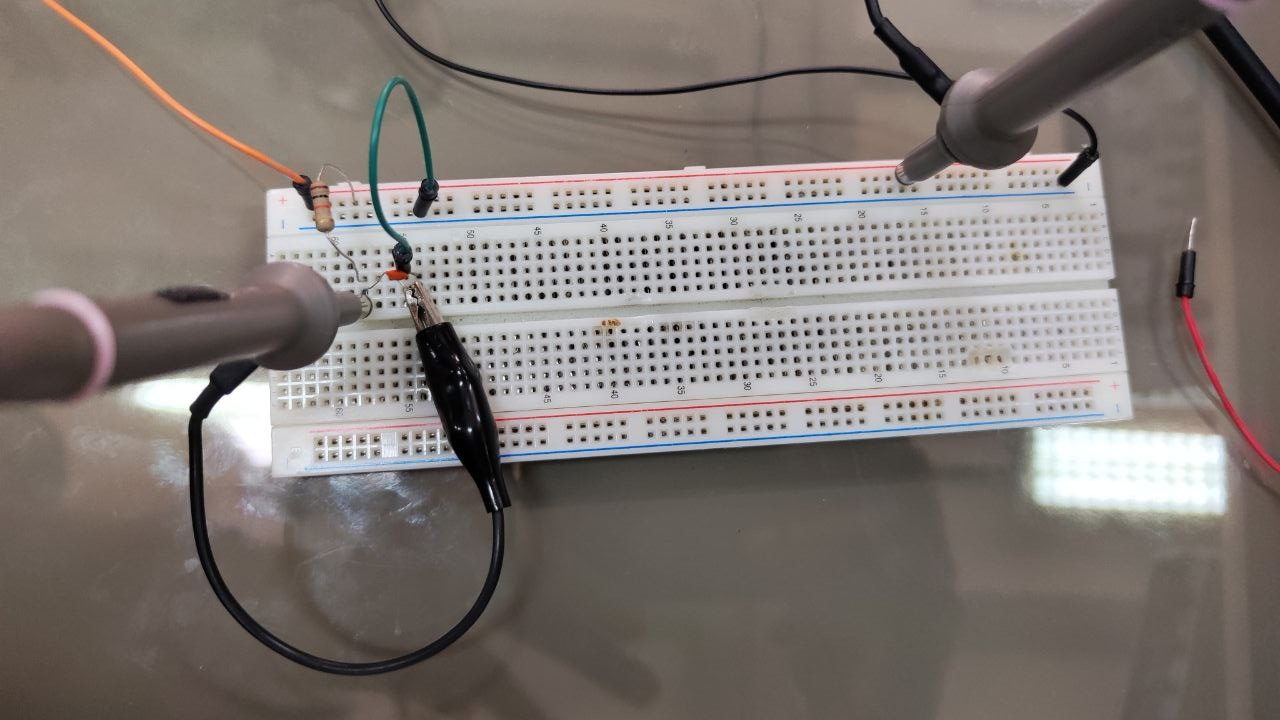
\includegraphics[scale=\PicScale,angle=0]{Fig/5.jpeg}
                \caption{The circuit.}
            \end{figure}
            \begin{figure}[H]
                \centering
                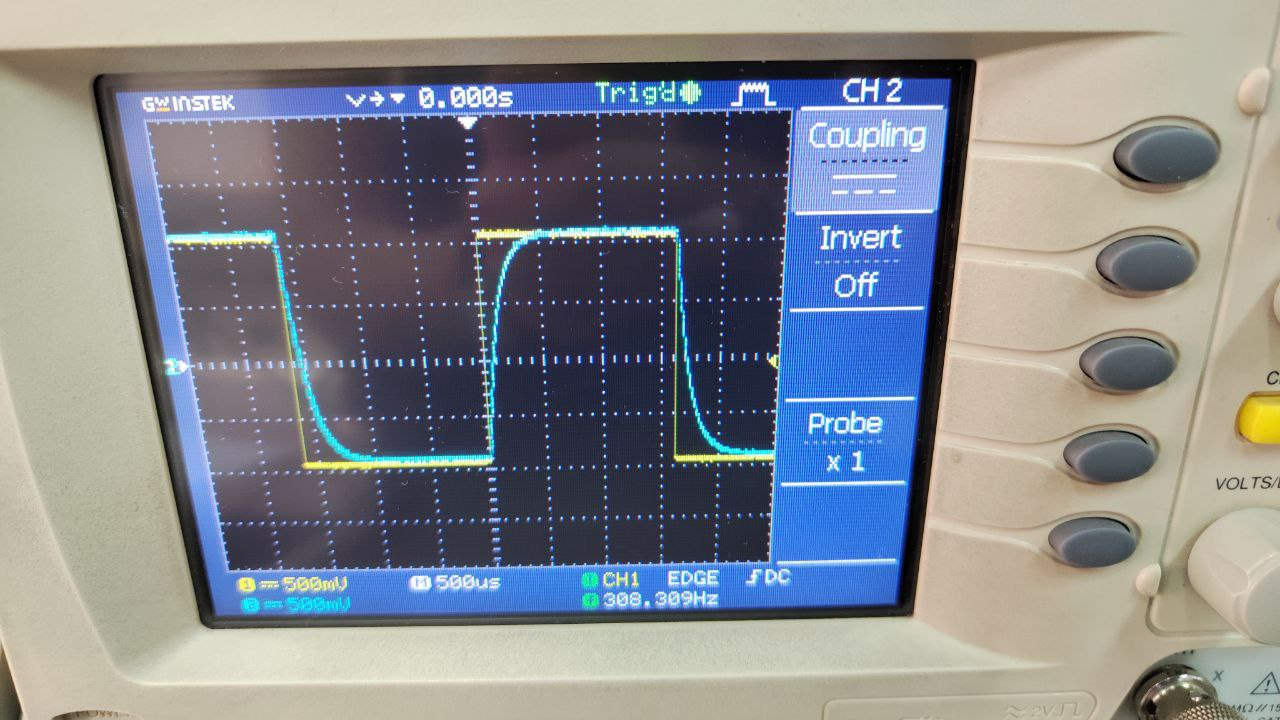
\includegraphics[scale=\PicScale,angle=0]{Fig/6.jpeg}
                \caption{The oscilloscope's screen.}
            \end{figure}

            Due to the presence of the capacitor, the circuit resists sudden changes, so when the square voltage changes, the circuit voltage changes smoothly. \\
            The time required to reach approximately $63\%$ of the maximum capacitor voltage is one $\tau$. So $\tau \cong 130\mu$. \\
            If we calculate the time constant using analytical methods, we need to calculate $R_{eq}C$. So:
            \[
                \tau_{analytical} = R_{eq}C = 10k \cdot 15n = 150\mu
            \]
            As expected, The two analytical and practical values are close.
        }
    \end{subquestion}

    %--------------------------------------------
    \begin{subquestion}{Apply a $1$-V sine wave to the input and change its frequency to measure the frequency response of the circuit using interpolation. See the input and output voltages simultaneously on the oscilloscope and discuss the filtering behavior of the circuit.}
        \answer{
            \begin{figure}[H]
                \centering
                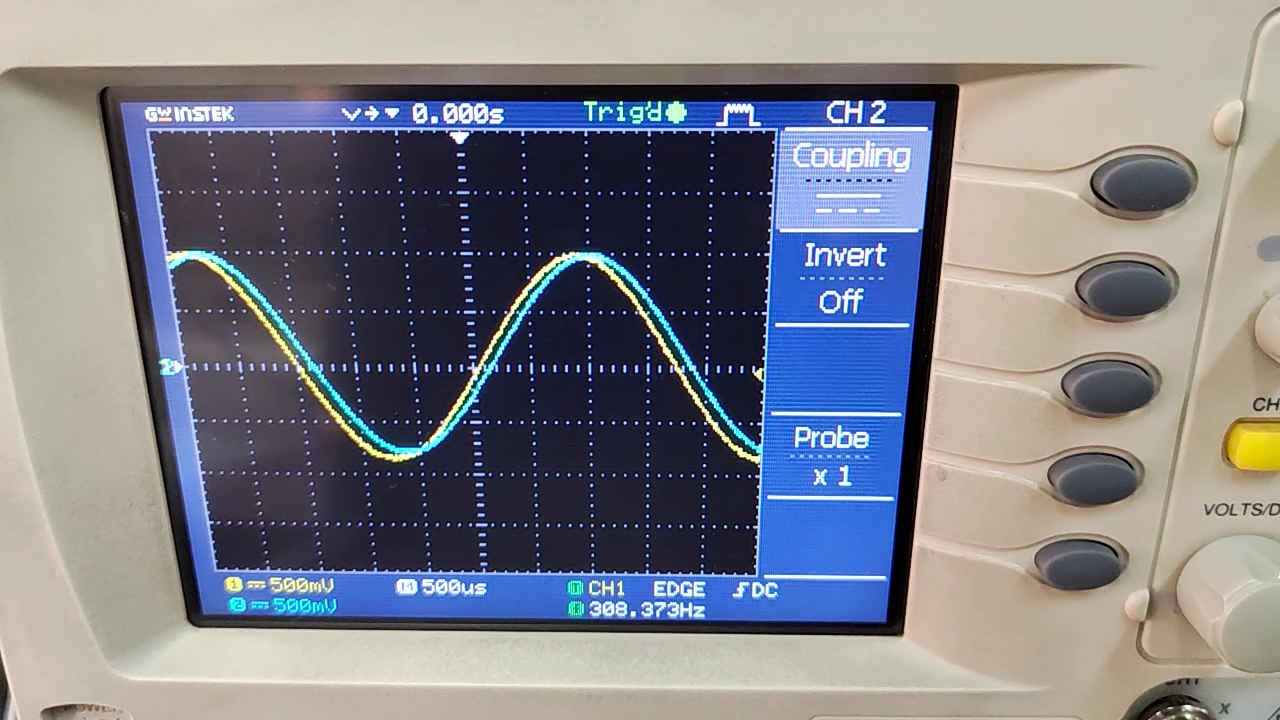
\includegraphics[scale=0.1,angle=0]{Fig/9.png}
                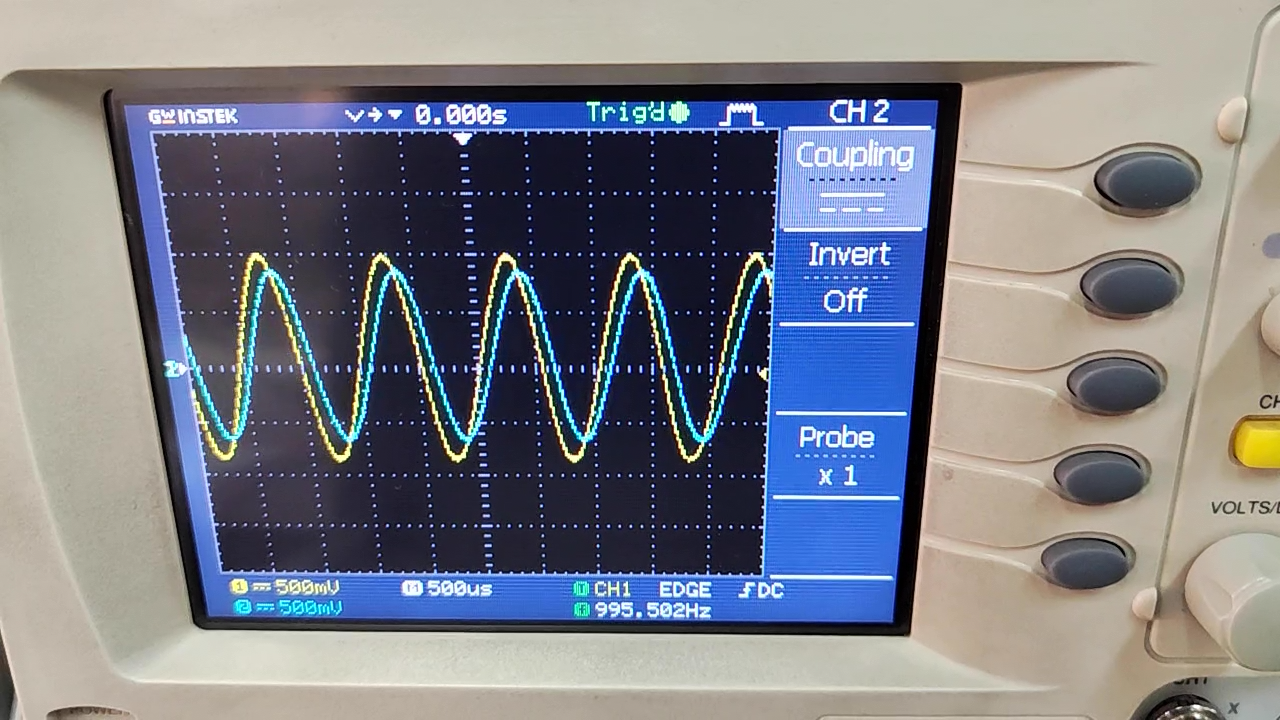
\includegraphics[scale=0.1,angle=0]{Fig/10.png}
                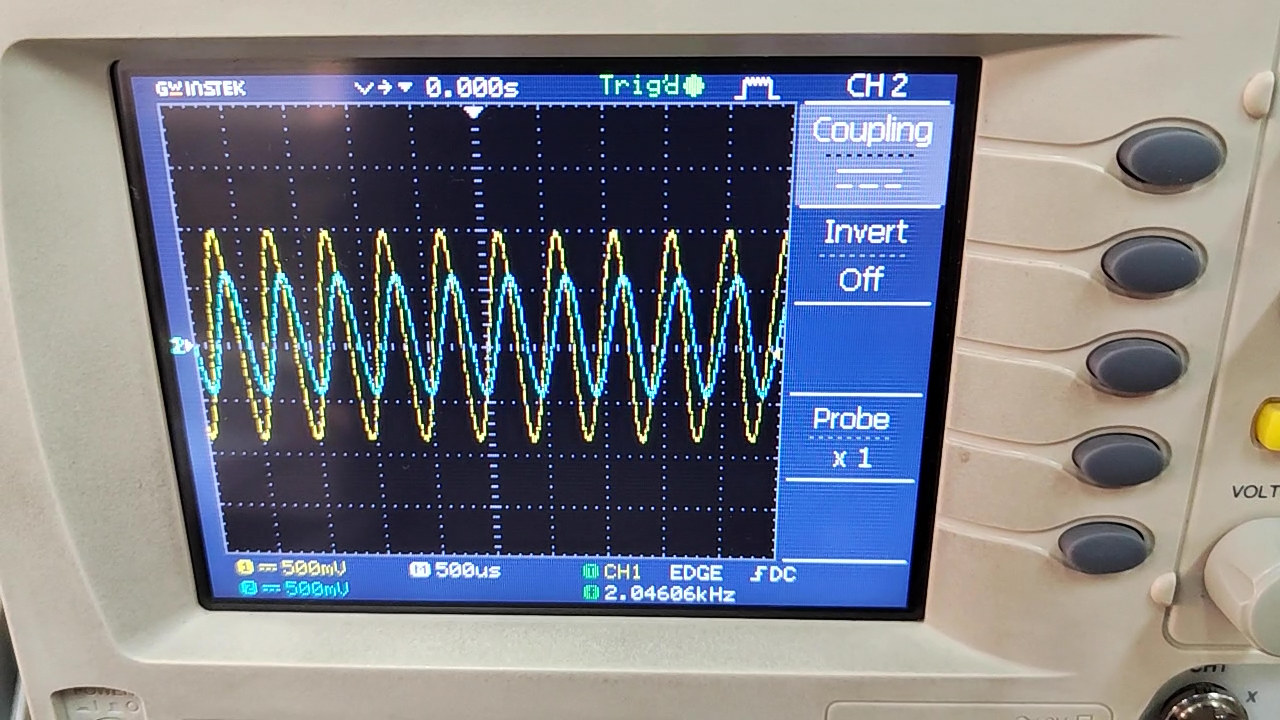
\includegraphics[scale=0.1,angle=0]{Fig/11.png}
                \caption{Circuit response to multiple input frequencies.}
            \end{figure}
            First of all, you can see some phase difference between the input and output voltage, which shows that the voltage at the two ends of the capacitor has a leading load compared to the input of the circuit.
            \[
                H(j\omega) = \frac{y_C}{y_{in}} = \frac{\frac{1}{15n j\omega}}{10k + \frac{1}{15n j\omega}} = \frac{1}{150 \times 10^{-6} j\omega + 1} = a - bj\omega
            \]
            This circuit is a low-pass filter, and for this reason, as shown in the pictures, a lower voltage is passed for higher frequencies.
        }
    \end{subquestion}


\end{question}

%----------------------------------------------------------------------------------------
%	QUESTION 3
%----------------------------------------------------------------------------------------

\begin{question}

    \questiontext{Build the circuit shown in Fig. \ref{fig:cir3} on a breadboard.}

    \begin{figure}[H]
        \centering
        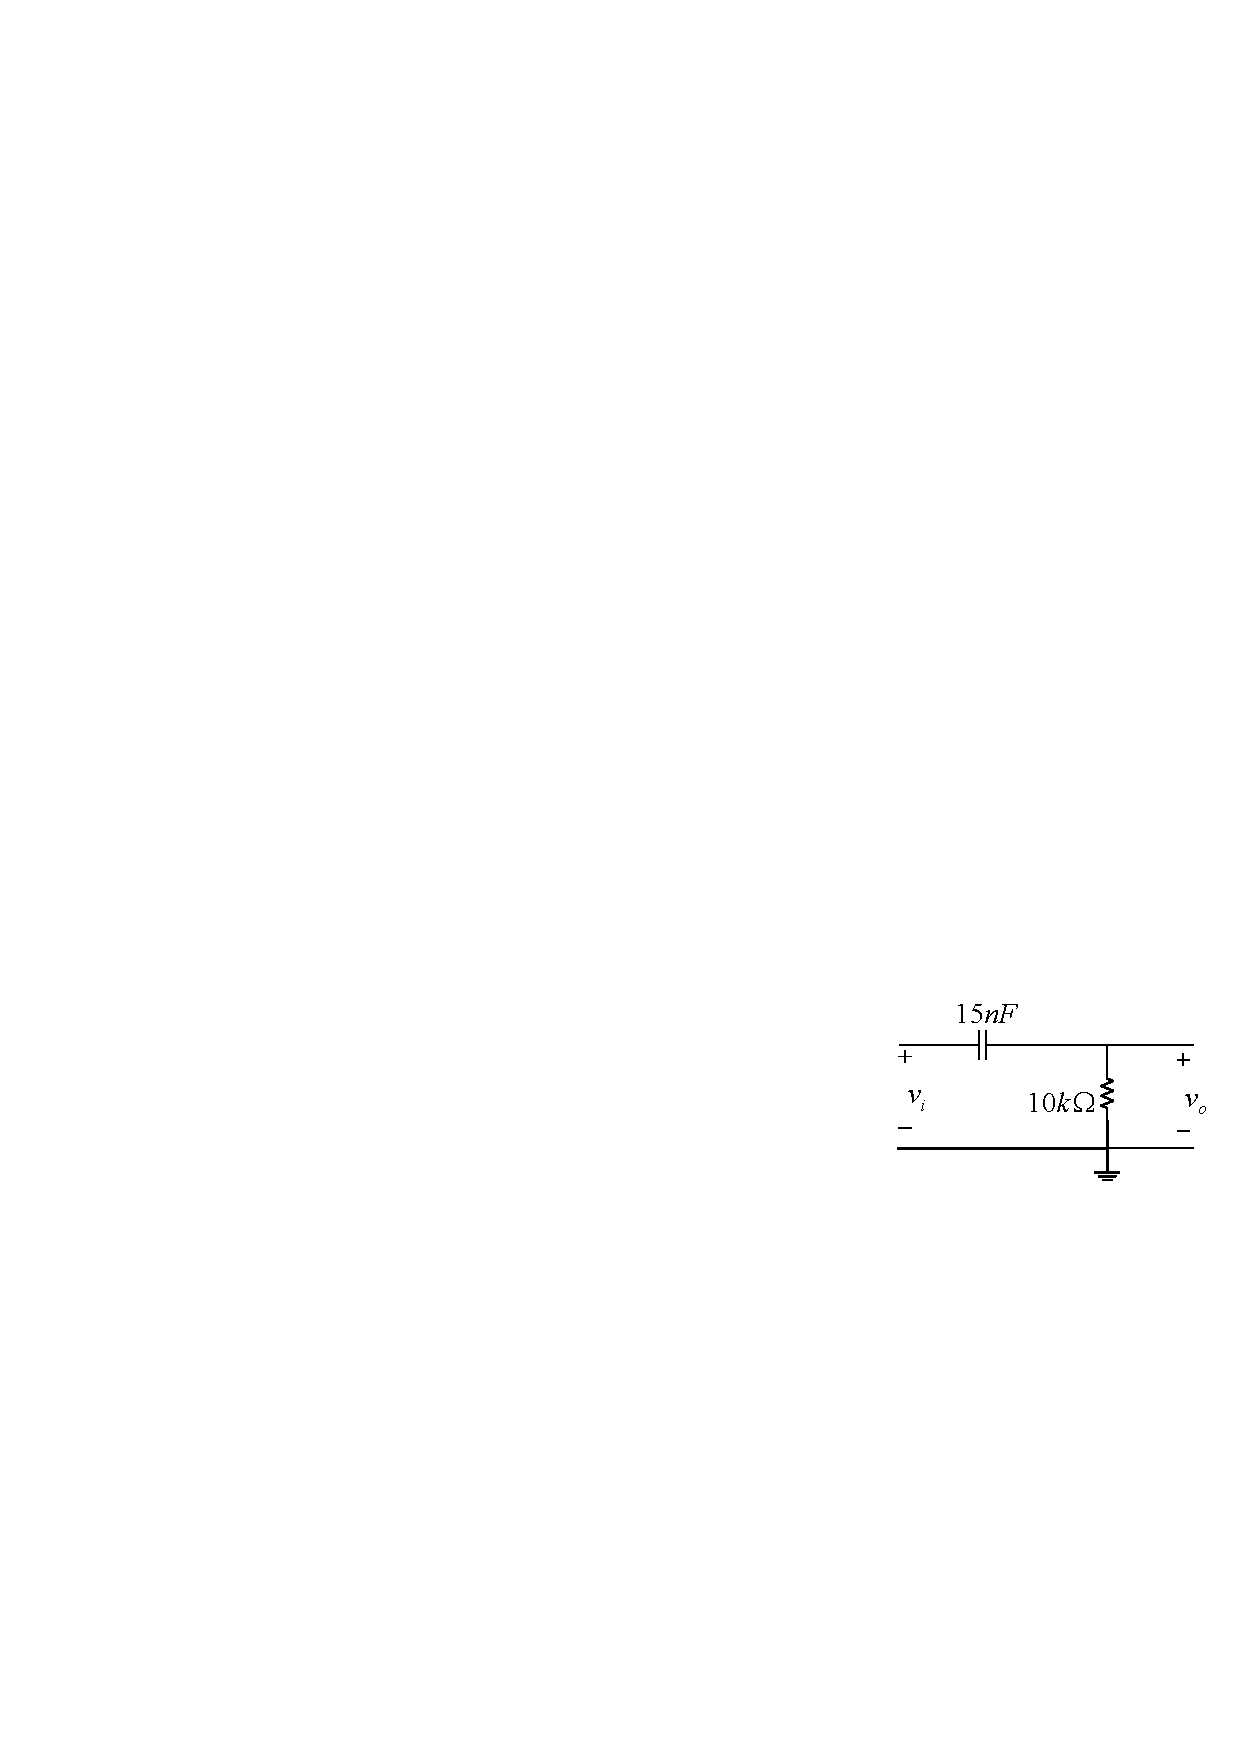
\includegraphics[scale=1.2,angle=0]{Fig/cir3.pdf}
        \caption{A highpass RC circuit.} \label{fig:cir3}
    \end{figure}

    %--------------------------------------------
    \begin{subquestion}{Apply a $1$-V $300$-Hz square wave to the input. See the input and output voltages simultaneously on the oscilloscope screen. Interpret the observations. Obtain the time constant of the circuit.}
        \answer{
            \begin{figure}[H]
                \centering
                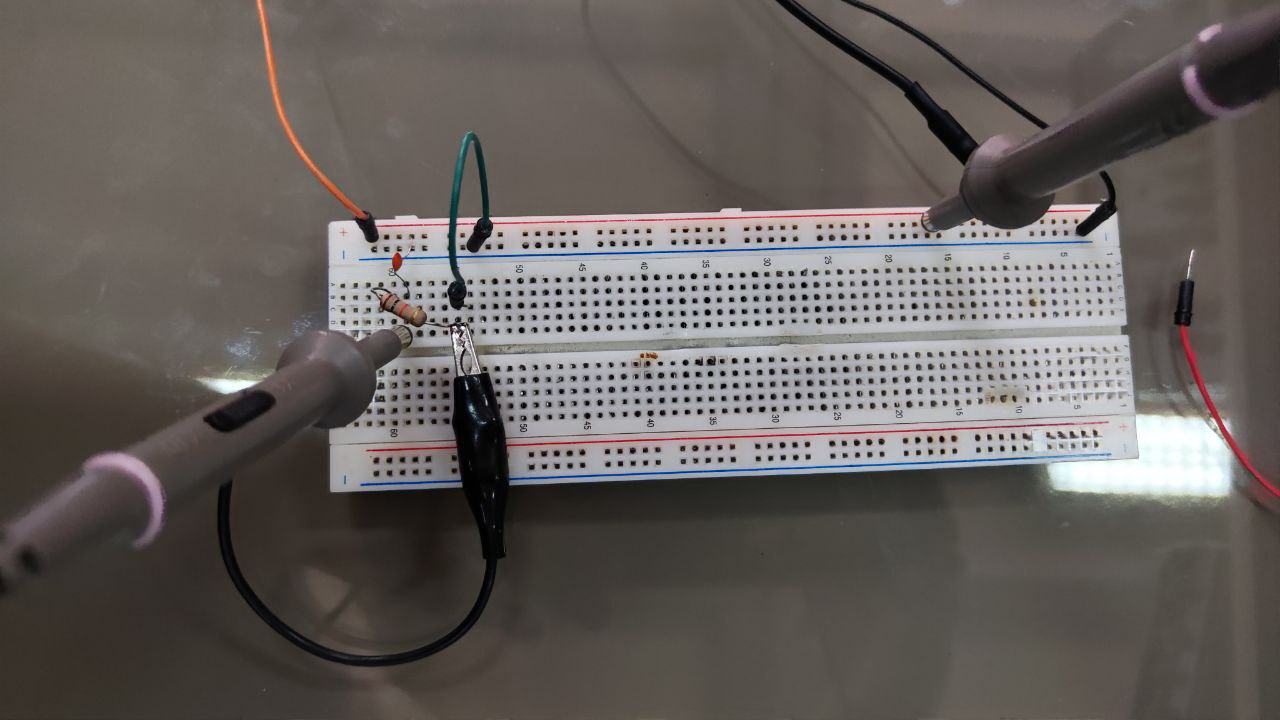
\includegraphics[scale=\PicScale,angle=0]{Fig/7.jpeg}
                \caption{The circuit.}
            \end{figure}
            \begin{figure}[H]
                \centering
                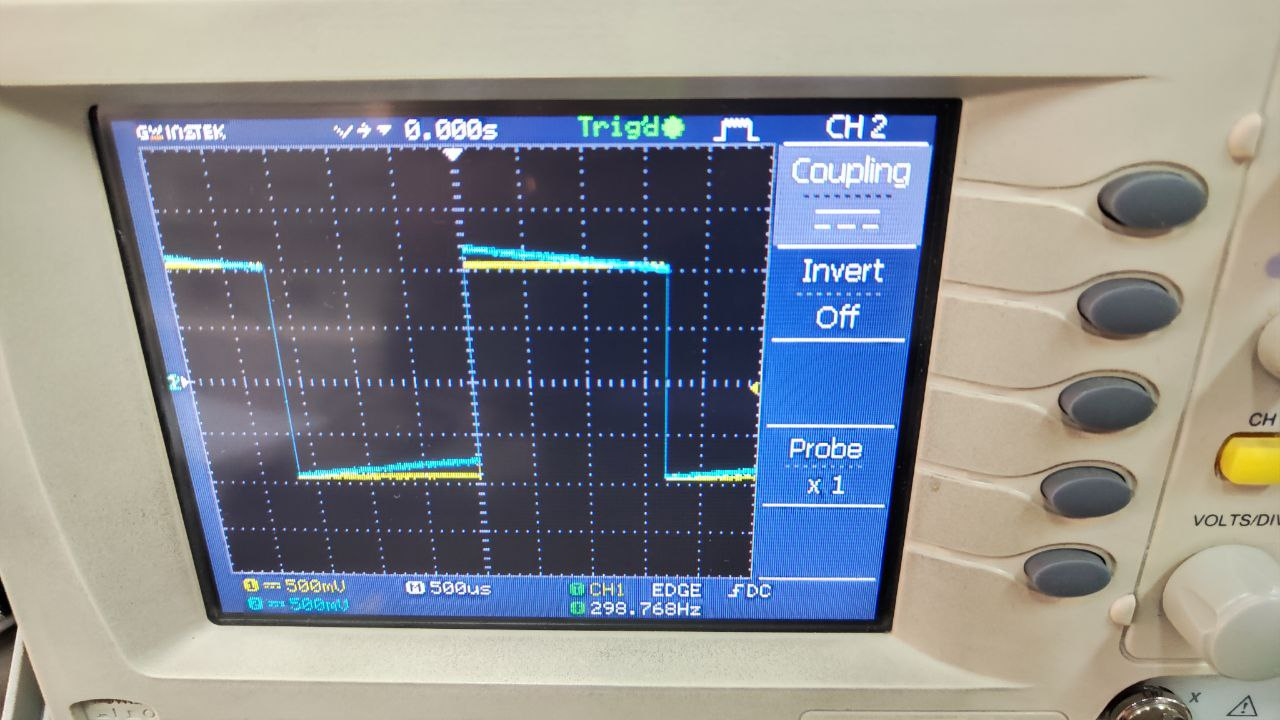
\includegraphics[scale=\PicScale,angle=0]{Fig/8.jpeg}
                \caption{The oscilloscope's screen.}
            \end{figure}

            When applying a positive voltage step initially, all the voltage is dropped across the resistor because the capacitor is empty. Gradually, the capacitor is charged and the voltage across it increases, and at the same time, the voltage across the resistor decreases. This process continues exponentially until the capacitor is fully charged. \\

            When a negative voltage step is applied, the previously charged capacitor must discharge in the opposite direction. At this moment, the voltage across the resistor drops suddenly. Because the capacitor cannot change the voltage instantaneously, so at the moment the input changes, all the voltage change falls on the resistor. This causes the voltage across the resistance to suddenly reach a negative value. After this sudden decrease, the capacitor starts to discharge. As the capacitor discharges, the voltage across the resistor gradually increases (moves toward zero). \\

            The time required for the capacitor voltage to decrease from its maximum value to approximately $37\%$ of that maximum is one $\tau$.
            So $\tau \cong 100\mu$.(Note that this descending part is not clear due to its smallness, so the obtained number is very imprecise) \\
            If we calculate the time constant using analytical methods, we need to calculate $R_{eq}C$. So:
            \[
                \tau_{analytical} = R_{eq}C = 10k \cdot 15n = 150\mu
            \]
            As expected, The two analytical and practical values are close.
        }
    \end{subquestion}

    %--------------------------------------------
    \begin{subquestion}{Apply a $1$-V sine wave to the input and change its frequency to measure the frequency response of the circuit using interpolation. See the input and output voltages simultaneously on the oscilloscope and discuss the filtering behavior of the circuit.}
        \answer{
            \begin{figure}[H]
                \centering
                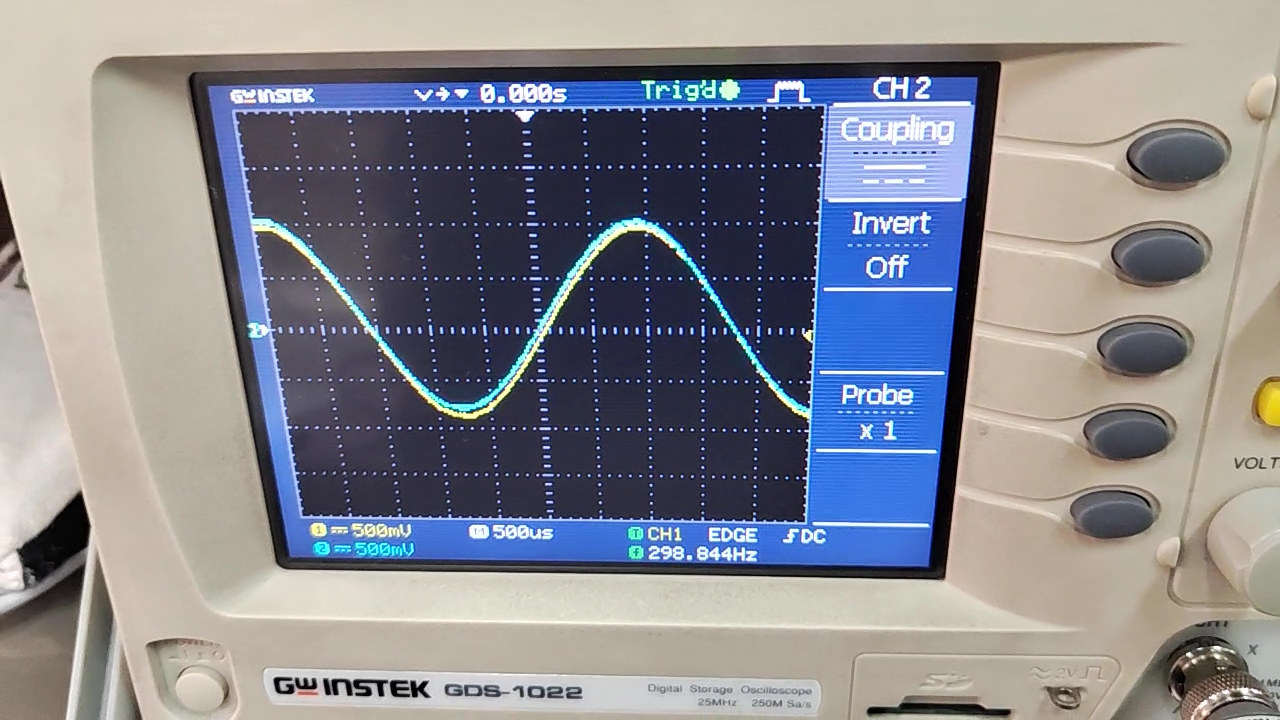
\includegraphics[scale=0.1,angle=0]{Fig/12.png}
                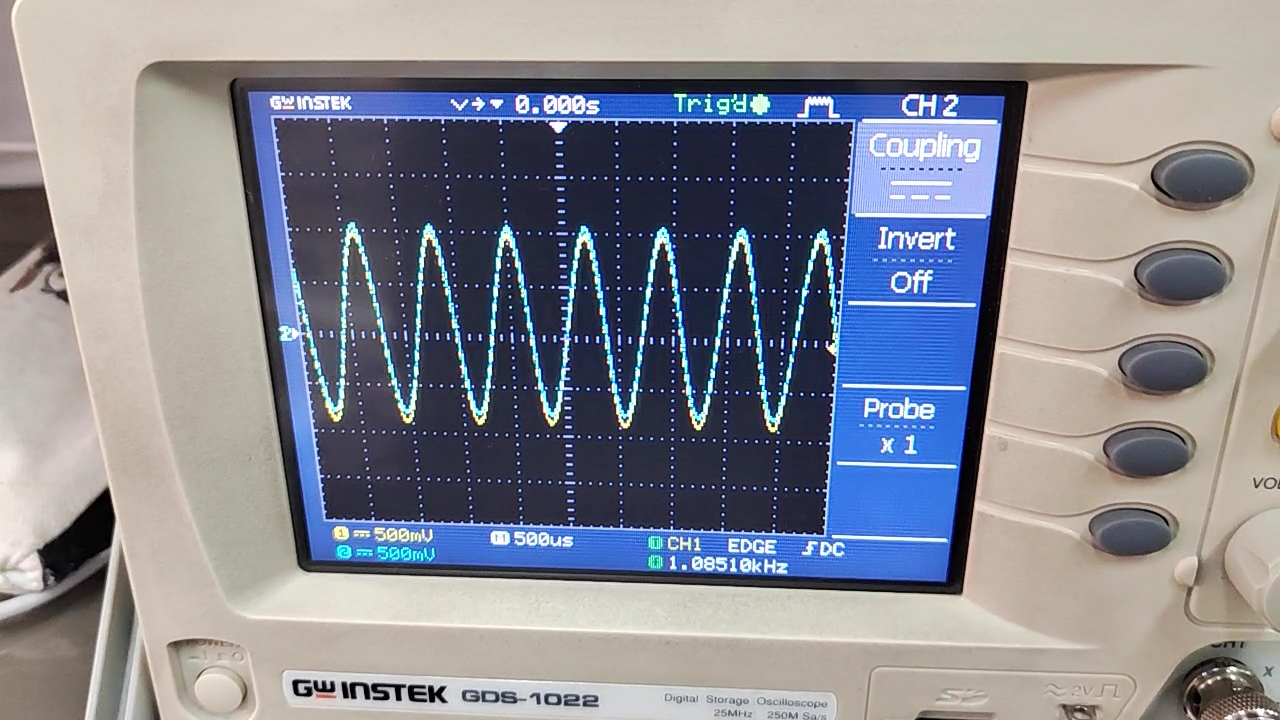
\includegraphics[scale=0.1,angle=0]{Fig/13.png}
                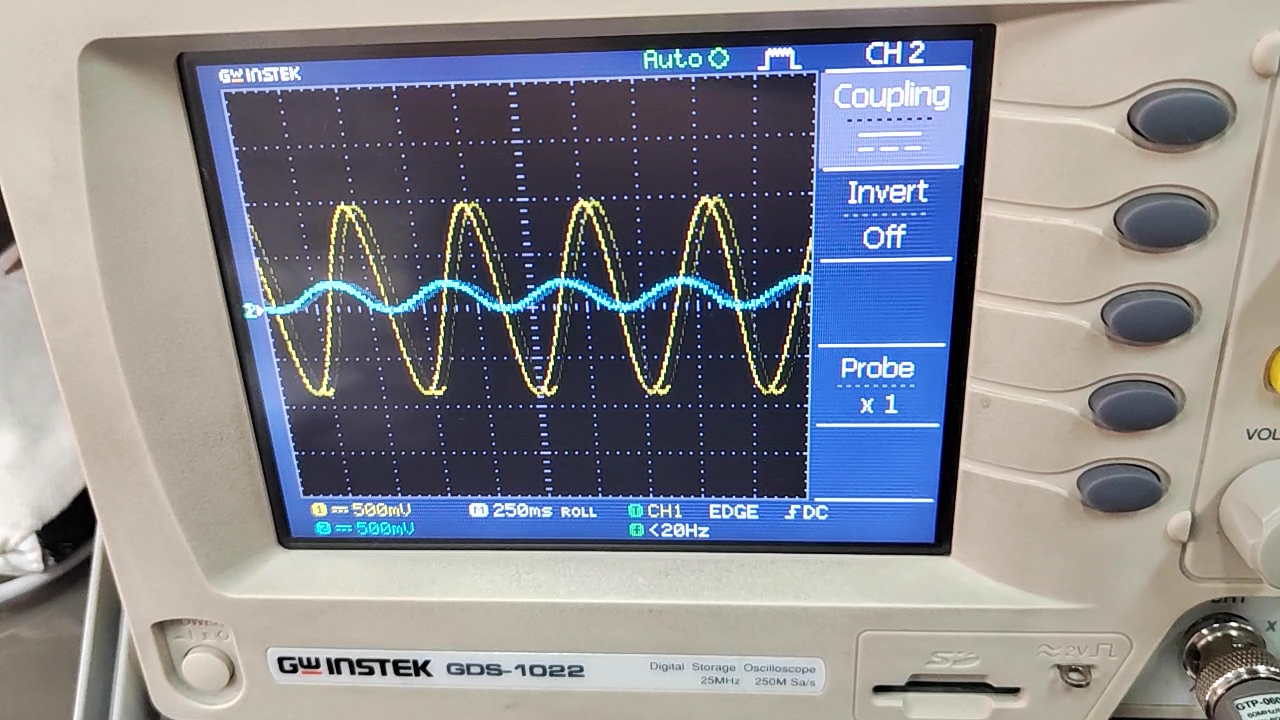
\includegraphics[scale=0.1,angle=0]{Fig/14.png}
                \caption{Circuit response to multiple input frequencies.}
            \end{figure}
            First of all, you can see some phase difference between the input and output voltage, which shows that the voltage at the two ends of the resistor has a lagging load compared to the input of the circuit.
            \[
                H(j\omega) = \frac{y_C}{y_{in}} = \frac{10k}{10k + \frac{1}{15n j\omega}} = \frac{150 \times 10^{-6} j\omega}{150 \times 10^{-6} j\omega + 1} = -a + bj\omega
            \]
            This circuit is a low-pass filter, and for this reason, as shown in the pictures, a lower voltage is passed for higher frequencies.
        }
    \end{subquestion}


\end{question}

%----------------------------------------------------------------------------------------
%	QUESTION 4
%----------------------------------------------------------------------------------------

\begin{question}

    \questiontext{Build the circuit shown in Fig. \ref{fig:cir4} on a breadboard.}

    \begin{figure}[H]
        \centering
        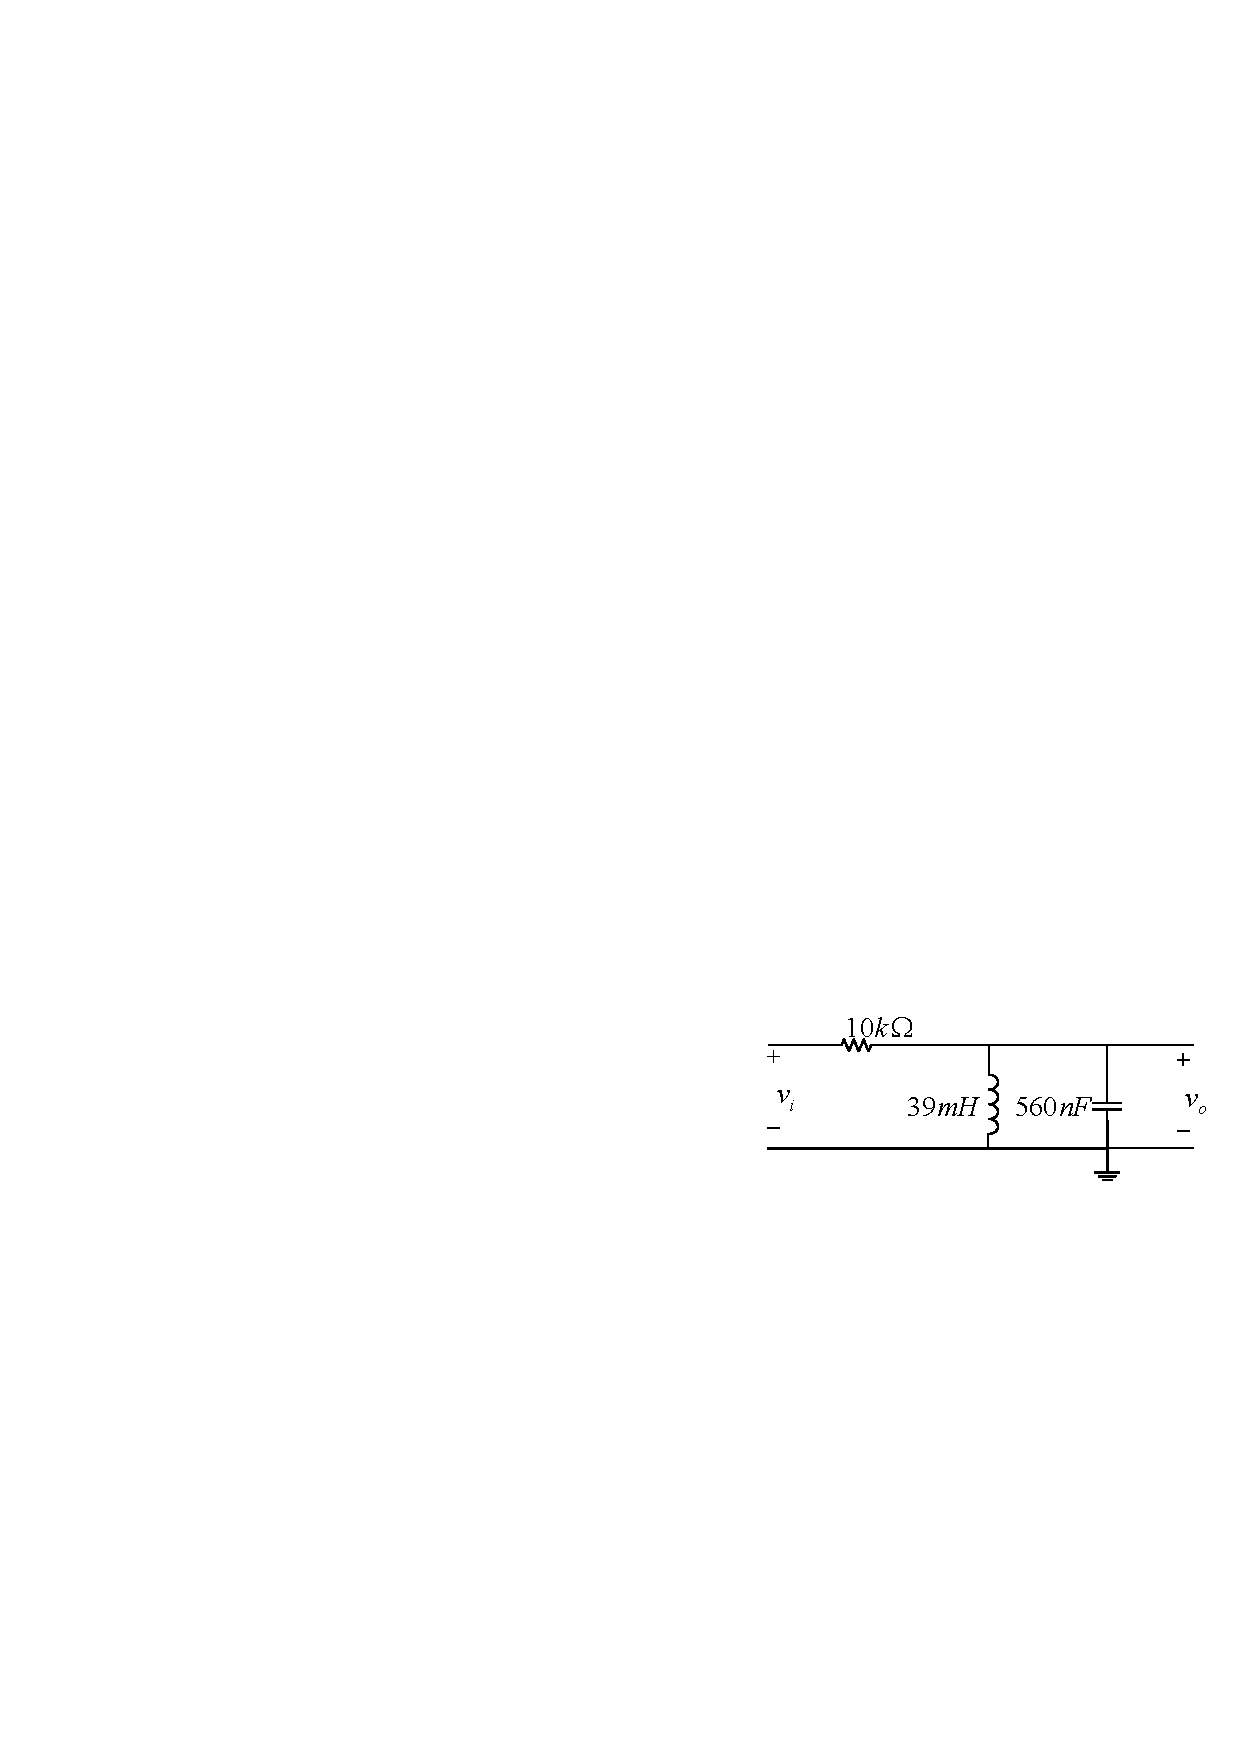
\includegraphics[scale=1.2,angle=0]{Fig/cir4.pdf}
        \caption{A bandpass RLC circuit.} \label{fig:cir4}
    \end{figure}

    %--------------------------------------------
    \begin{subquestion}{Apply a $1$-V sine wave to the input and change its frequency from $100$ Hz to $10$ kHz to measure the frequency response of the circuit using interpolation. See the input and output voltages simultaneously on the oscilloscope and discuss the filtering behavior of the circuit.}
        \answer{
            \begin{figure}[H]
                \centering
                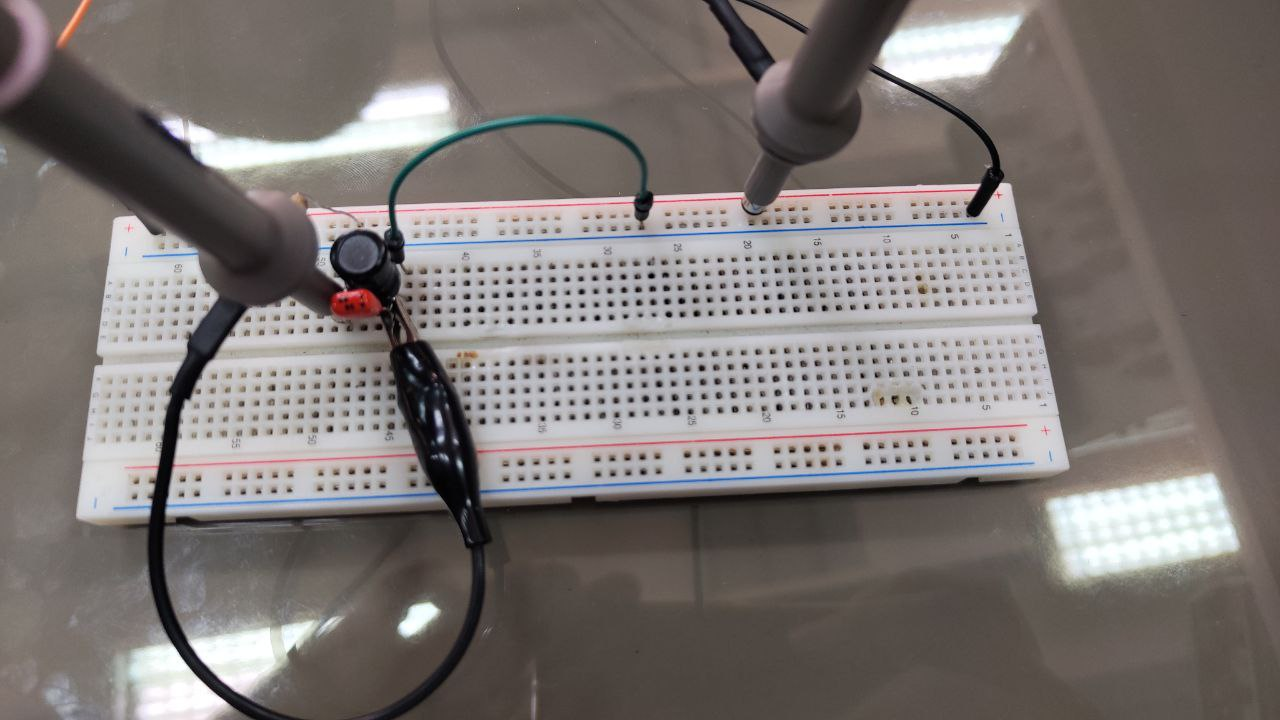
\includegraphics[scale=\PicScale,angle=0]{Fig/15.jpeg}
                \caption{The circuit.}
            \end{figure}
            \begin{figure}[H]
                \centering
                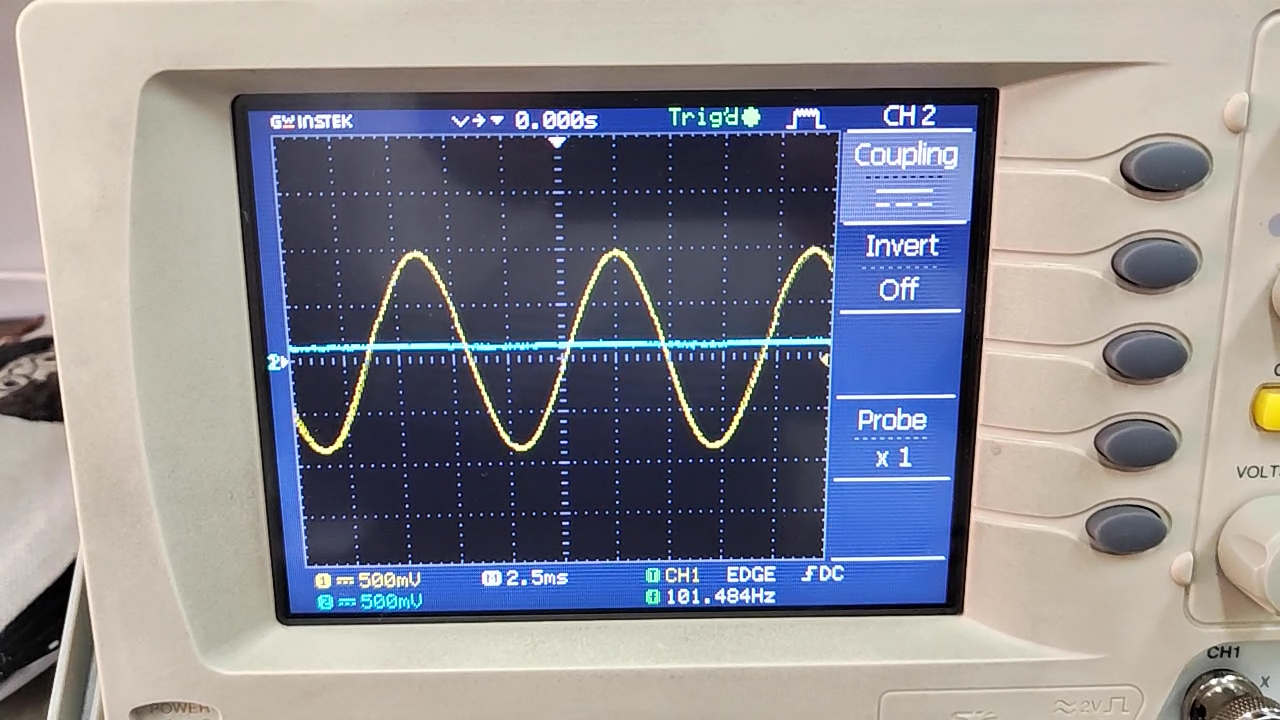
\includegraphics[scale=0.1,angle=0]{Fig/16.png}
                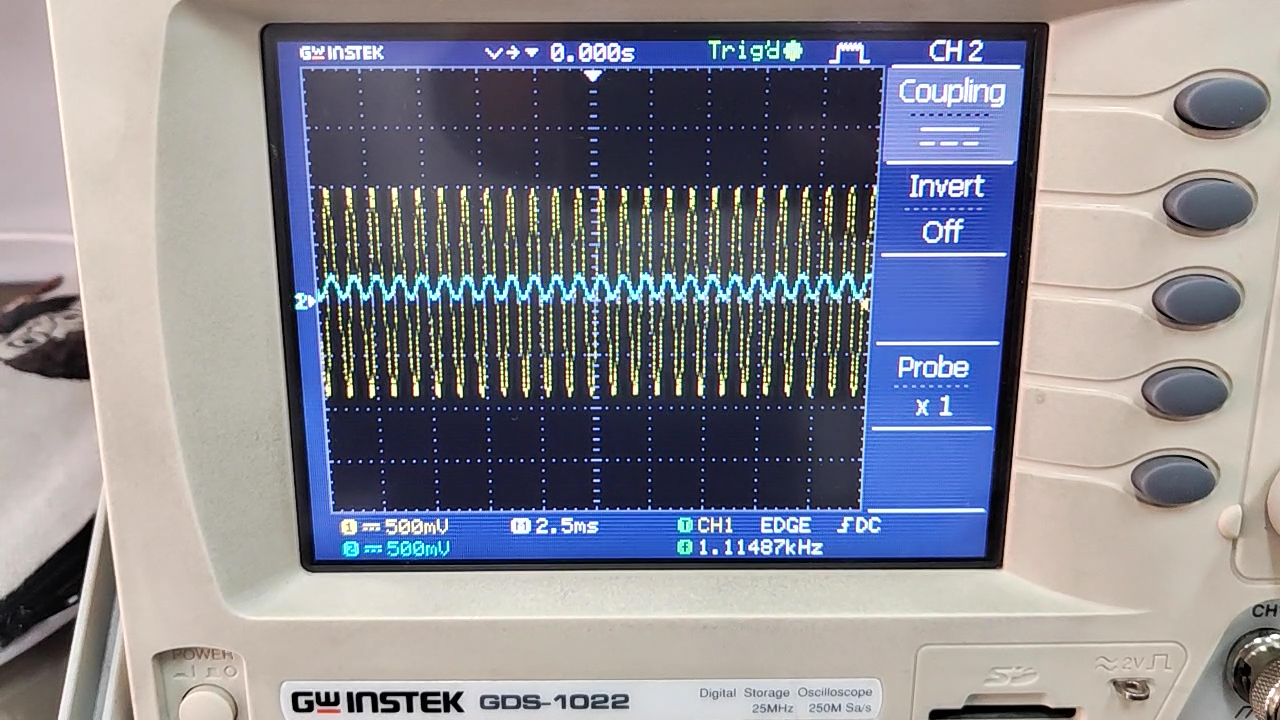
\includegraphics[scale=0.1,angle=0]{Fig/17.png}
                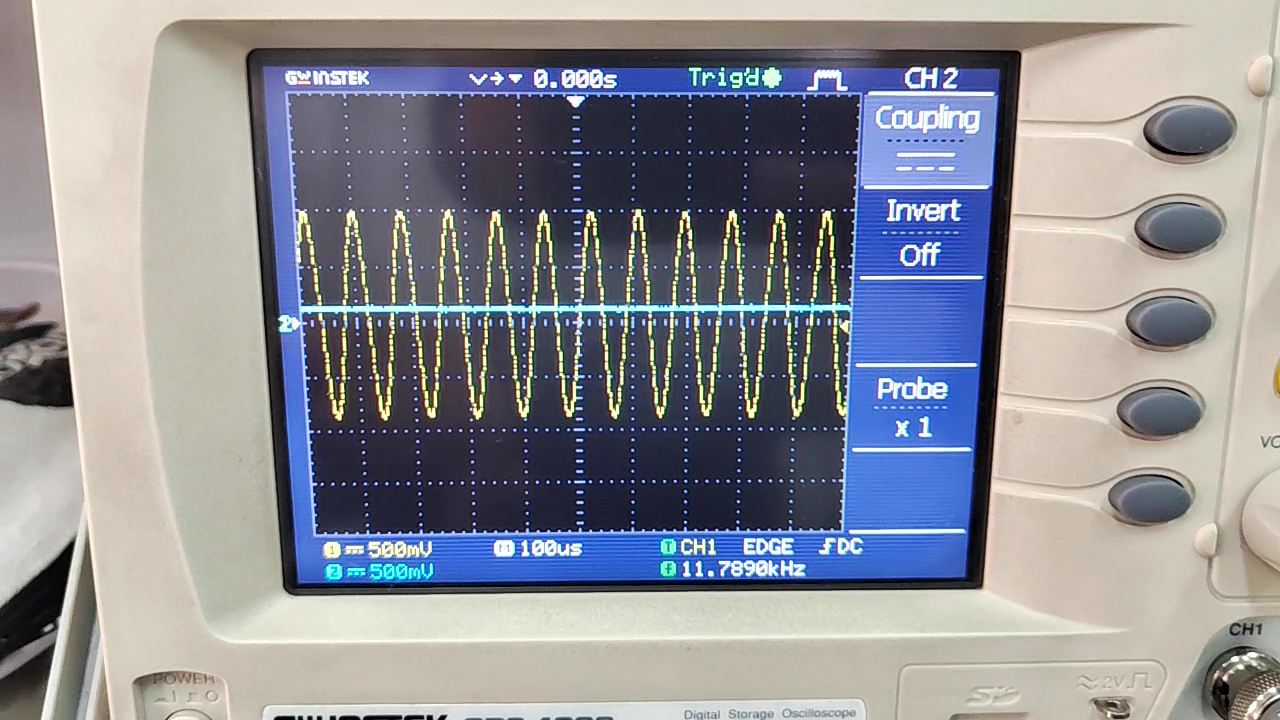
\includegraphics[scale=0.1,angle=0]{Fig/18.png}
                \caption{Circuit response to multiple input frequencies}
            \end{figure}
            \begin{figure}[H]
                \centering
                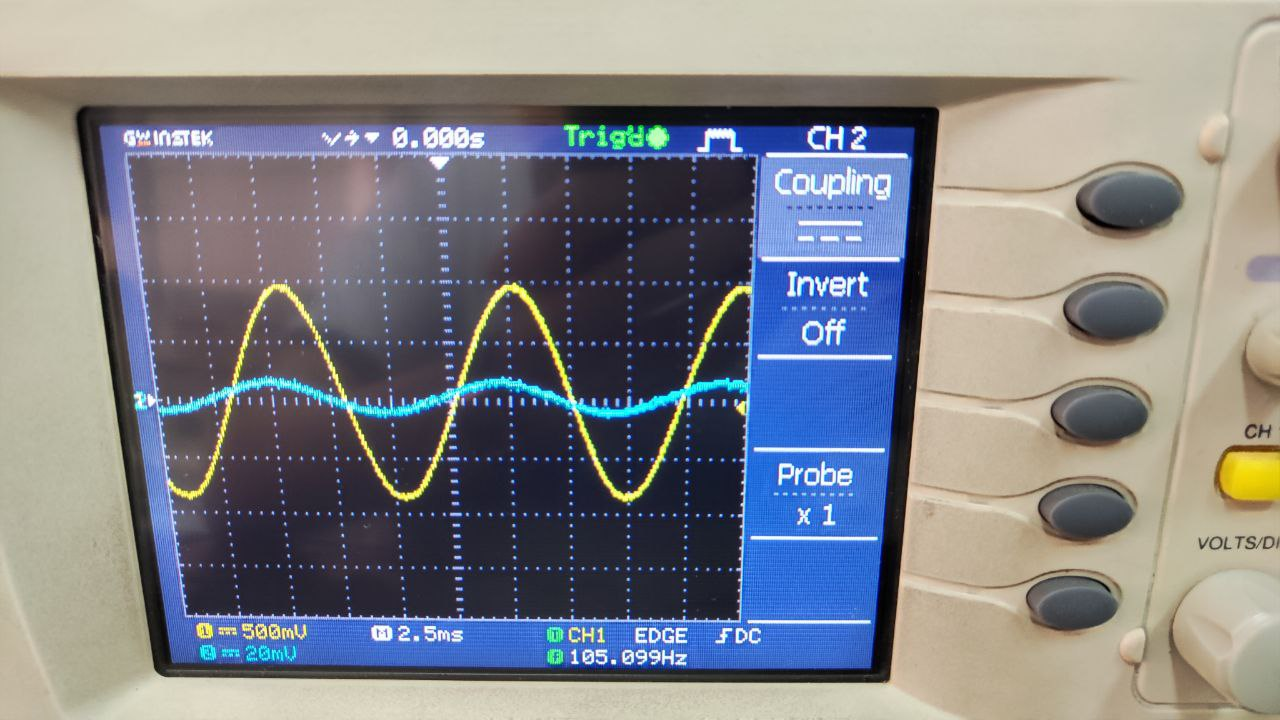
\includegraphics[scale=0.1,angle=0]{Fig/19.jpeg}
                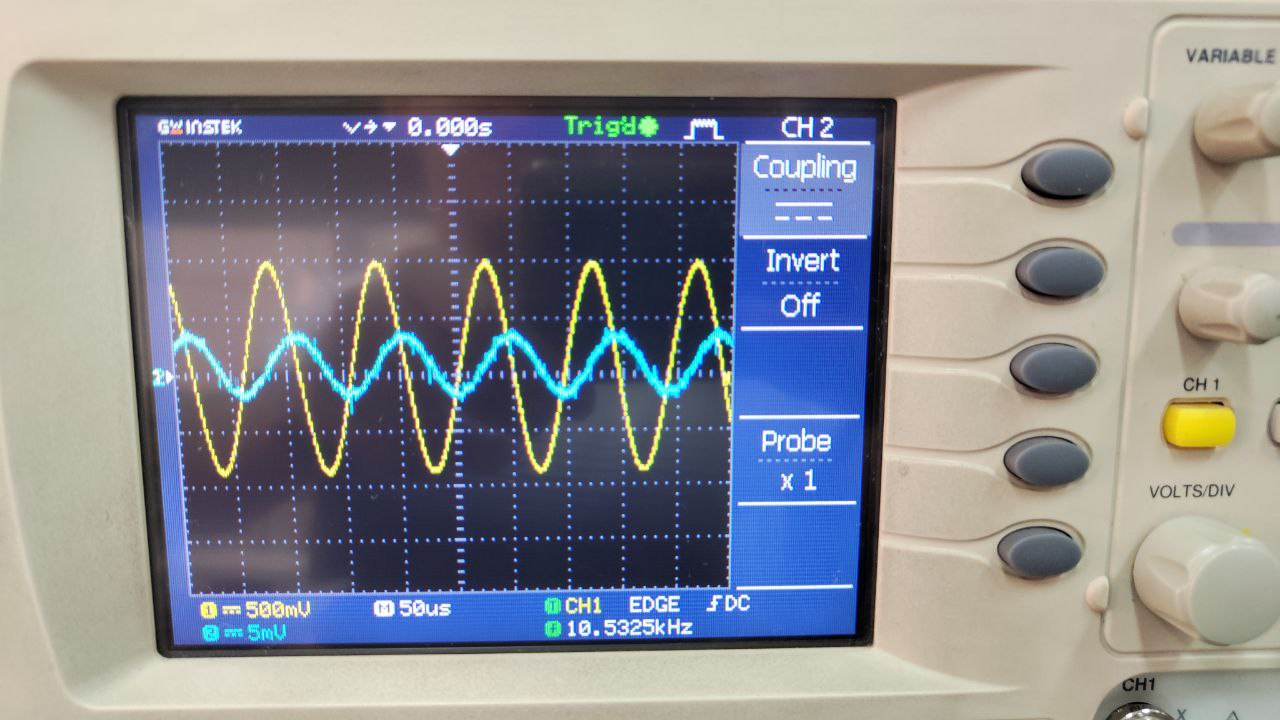
\includegraphics[scale=0.1,angle=0]{Fig/20.jpeg}
                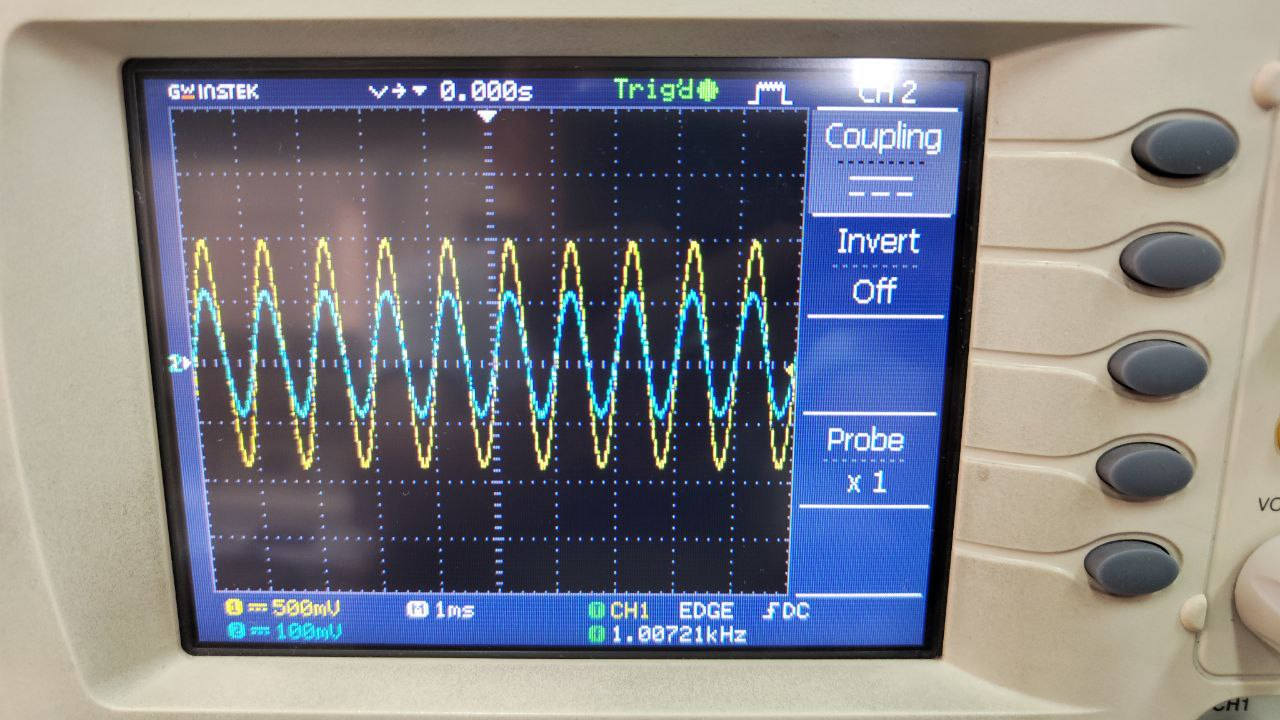
\includegraphics[scale=0.1,angle=0]{Fig/21.jpeg}
                \caption{Volt/div has been reduced to better display the amount of passing voltage.}
            \end{figure}
            As you can see, due to the fact that this is a bandpass filter, the voltage corresponding to the $1K$ frequency is better passed between the three frequencies, $100$, $1K$ and $11K$. (In the next three photos, the graph of all three states is zoomed, which shows that a small amount of voltage passes in each state)
        }
    \end{subquestion}

    %--------------------------------------------
    \begin{subquestion}{Apply a $1$-V square wave to the input and sweep its frequency from $100$ Hz to $10$ kHz. See the input and output voltages simultaneously on an oscilloscope screen. Interpret the observations.}
        \answer{
            \begin{figure}[H]
                \centering
                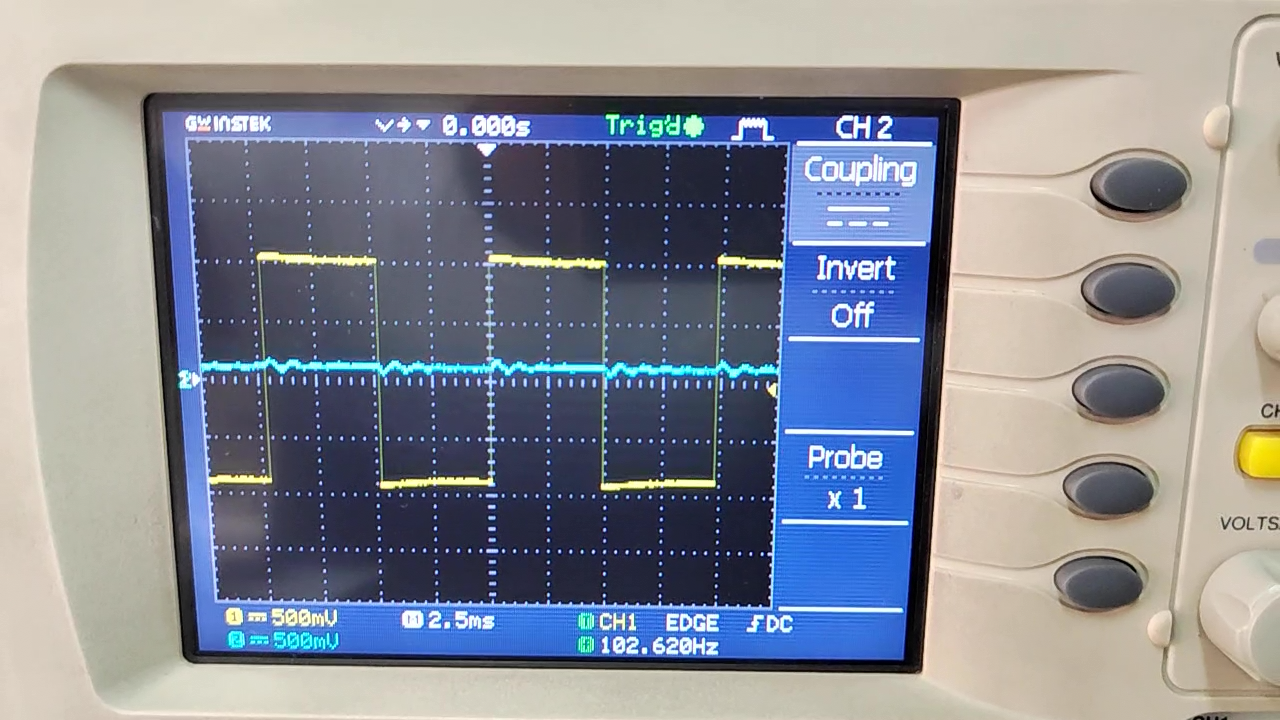
\includegraphics[scale=0.1,angle=0]{Fig/22.png}
                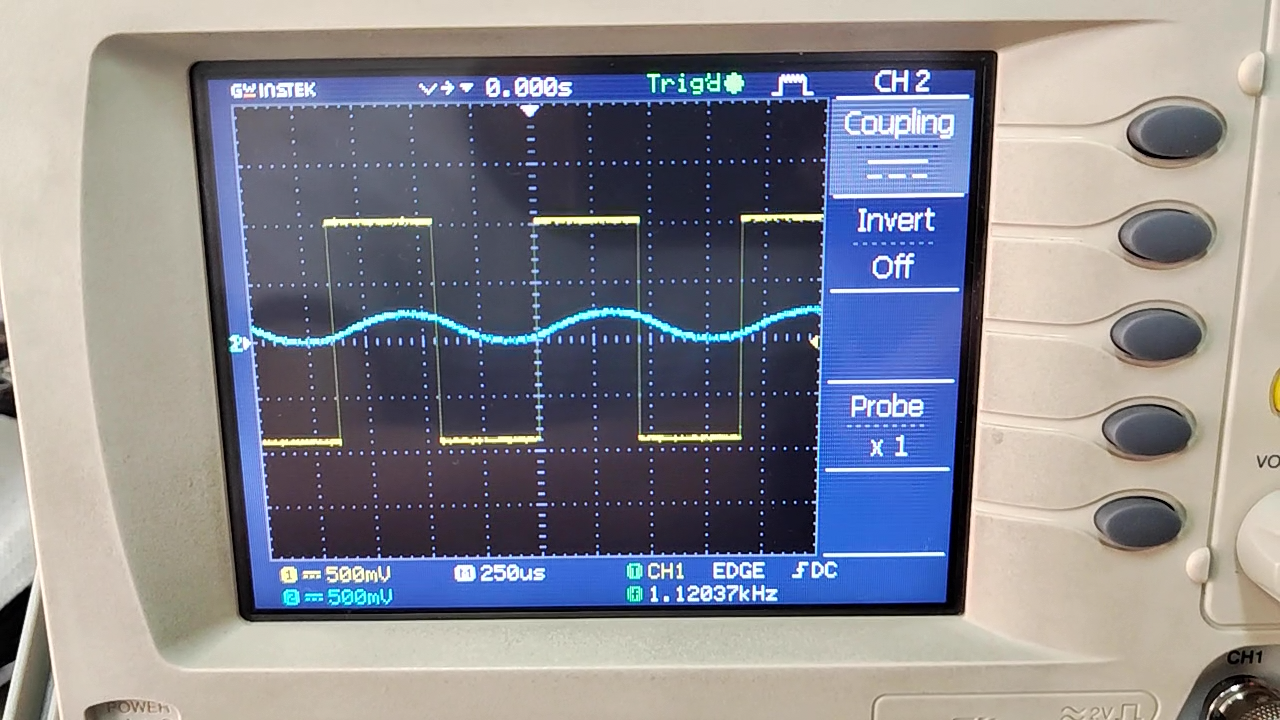
\includegraphics[scale=0.1,angle=0]{Fig/23.png}
                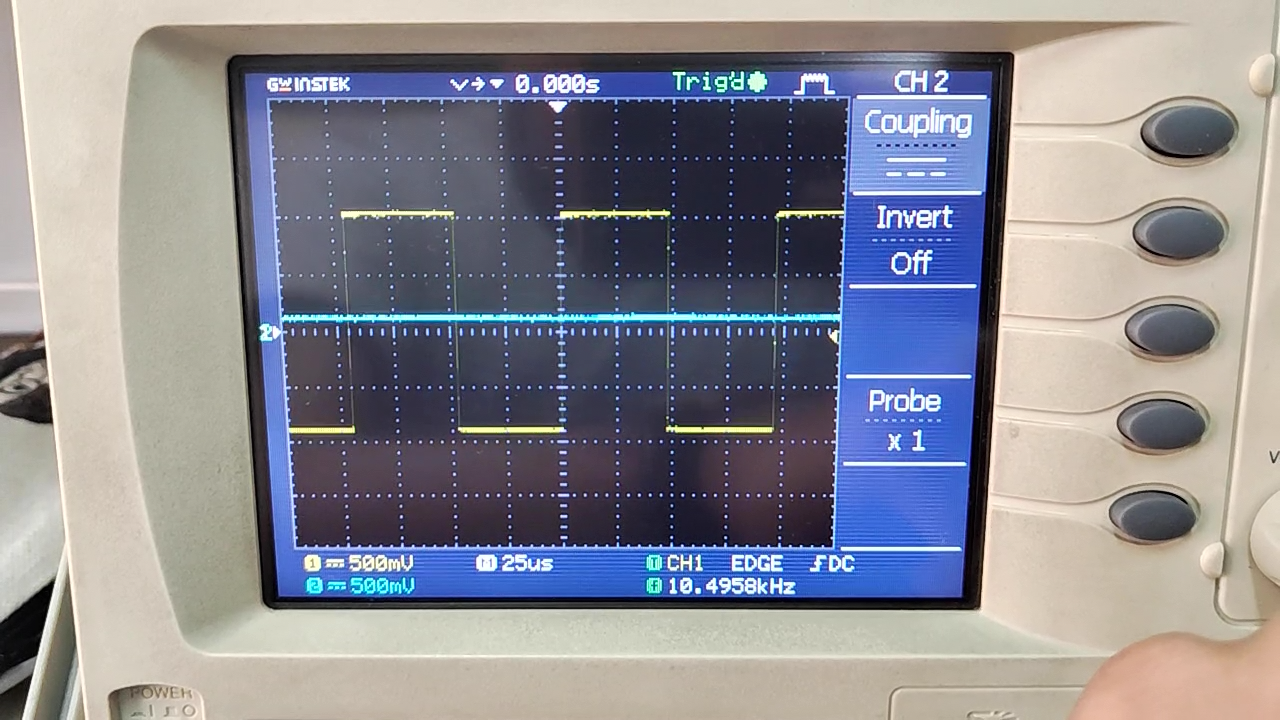
\includegraphics[scale=0.1,angle=0]{Fig/24.png}
                \caption{Circuit response to multiple input frequencies}
            \end{figure}
            \begin{figure}[H]
                \centering
                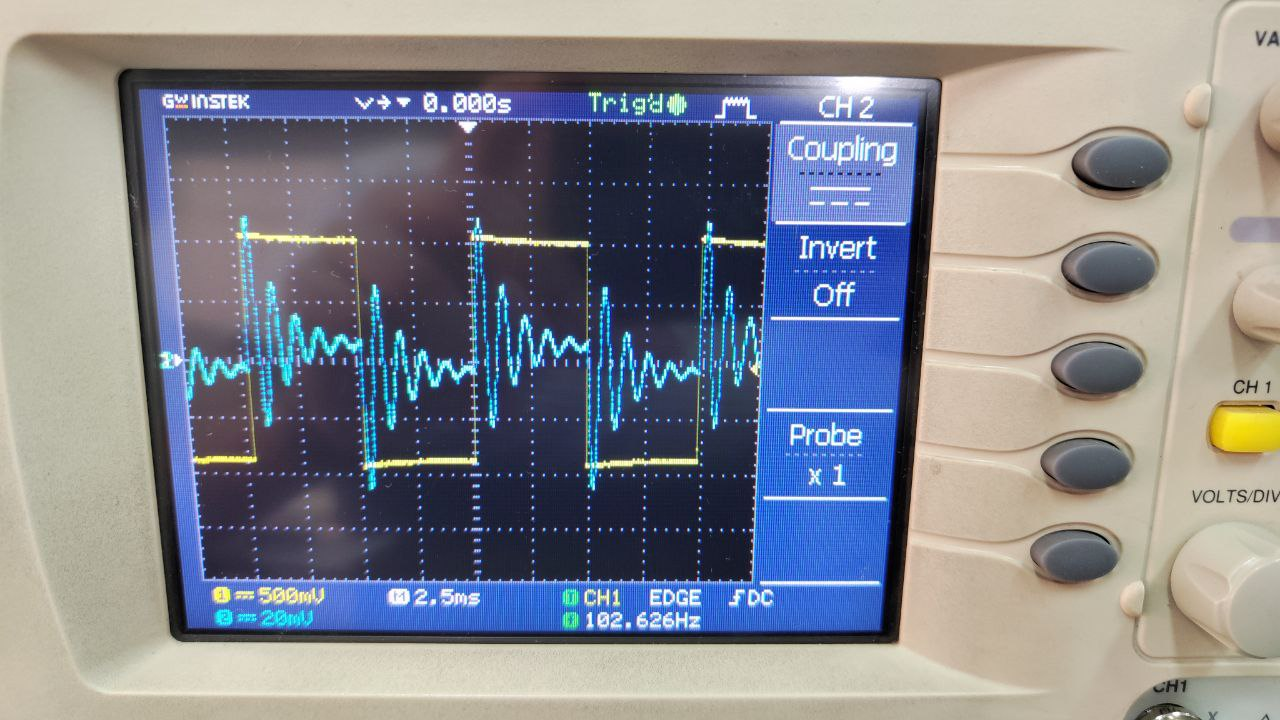
\includegraphics[scale=0.1,angle=0]{Fig/25.jpeg}
                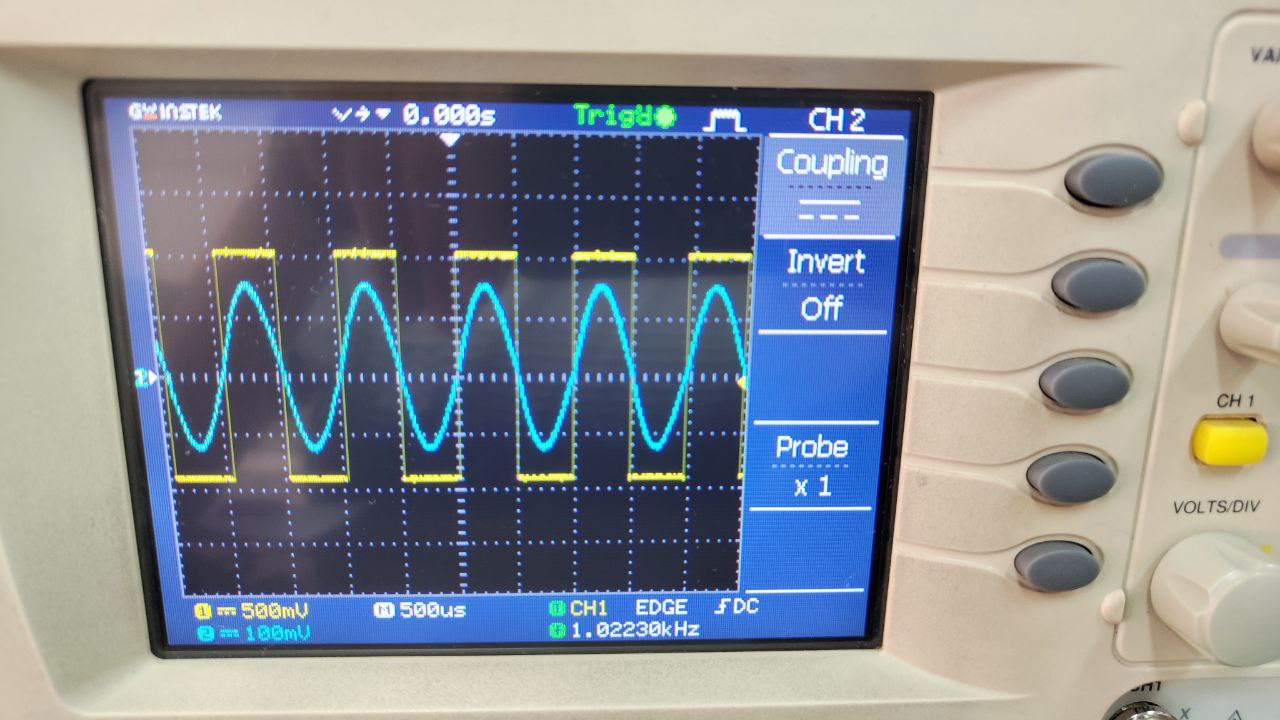
\includegraphics[scale=0.1,angle=0]{Fig/26.jpeg}
                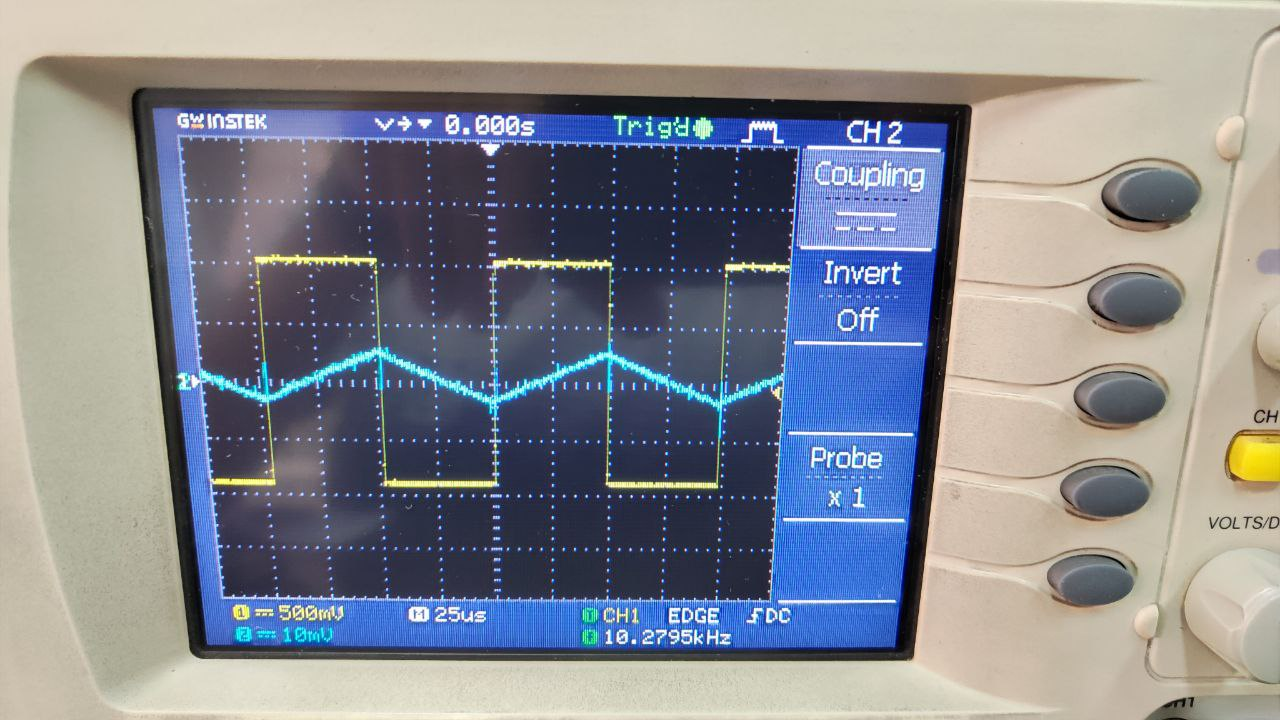
\includegraphics[scale=0.1,angle=0]{Fig/27.jpeg}
                \caption{Volt/div has been reduced to better display the amount of passing voltage.}
            \end{figure}
            Similar to the previous case, you can see that the filter passes the voltage related to the $1K$ frequency better. \\

            In this case, by focusing on the voltage graphs, it can be seen that these passing frequencies have a sinusoidal state. The reason for this is that, based on the Fourier transform, a square wave is composed of several sine waves with different frequencies, so when this wave passes through a bandpass filter, the sine waves with low and high frequencies are attenuated. And sine waves with medium frequencies pass, and for this reason, the output wave has a sinusoidal shape.
        }
    \end{subquestion}

\end{question}


\assignmentSection{Bonus Experiments}

%----------------------------------------------------------------------------------------
%	QUESTION 5
%----------------------------------------------------------------------------------------

\begin{question}

    \questiontext{The circuit shown in Fig. \ref{fig:Q5} is called Sallen active lowpass filter, where the triangle abstracts an op-amp amplification circuit with the gain $K$.}

    \begin{figure}[H]
        \begin{center}
            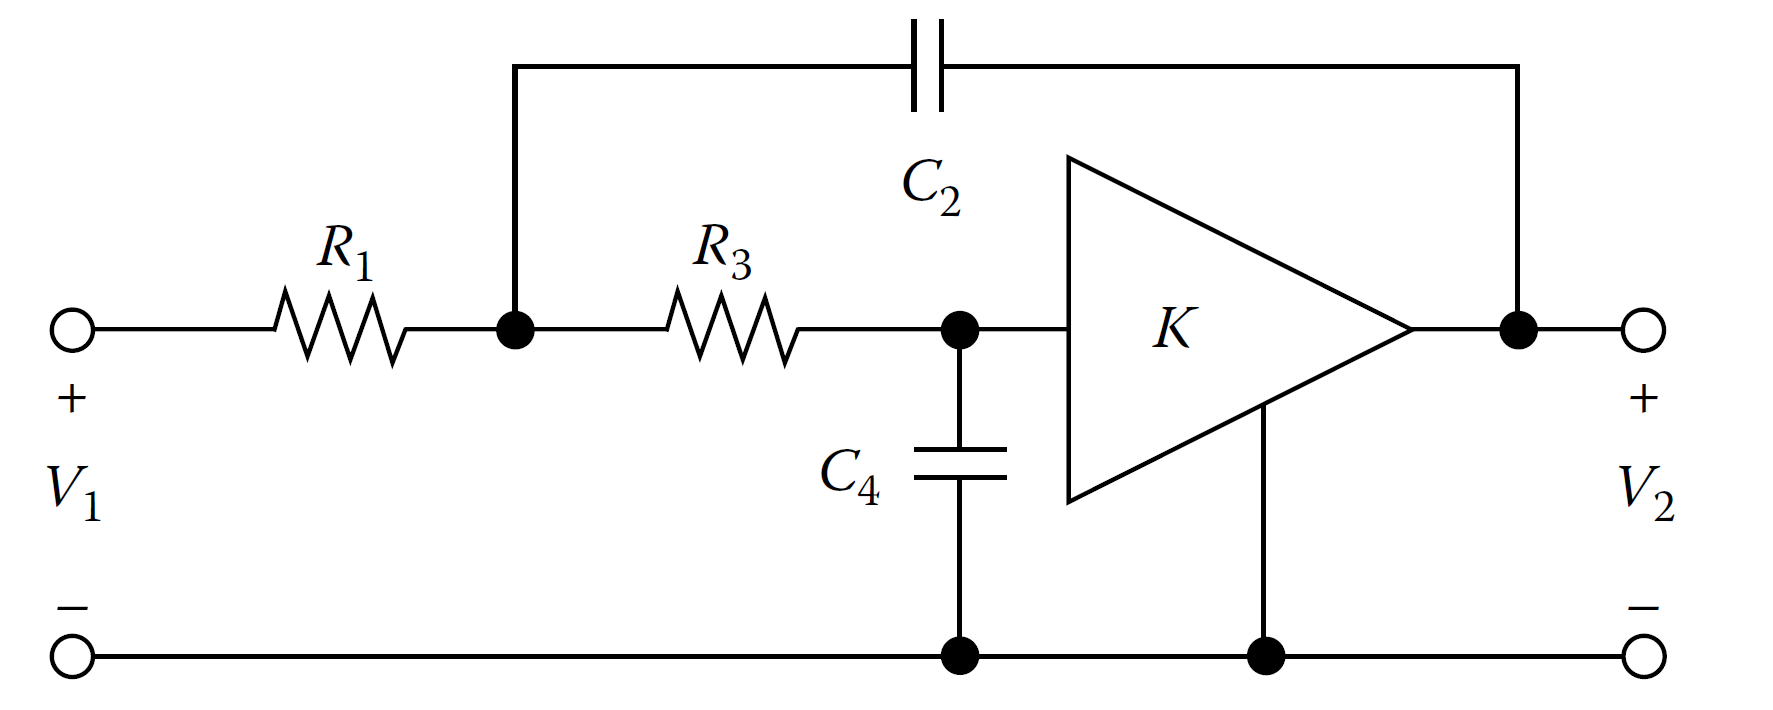
\includegraphics[scale=0.3]{Fig/Q5.png}
            \caption{\label{fig:Q5} Sallen active lowpass filter.}
        \end{center}
    \end{figure}

    %--------------------------------------------
    \begin{subquestion}{Calculate the frequency response of the active filter circuit.}
        \answer{
            The gain of the op-amp is K then the input voltage of the amplifier is $\frac{V_2}{K}$.
            Now let's denote the node between $R_1 , R_3 , C_2$ as $V$. so, from the KCL:
            \[
                \begin{cases}
                    \frac{V - V_1}{R_1} + C_2 j\omega (V - V_2) + \frac{V - \frac{V_2}{K}}{R_3} = 0 \\
                    \frac{\frac{V_2}{K} - V}{R_3} + C_4 j\omega \frac{V_2}{K} = 0 \Rightarrow V = \frac{V_2}{K} + R_3 C_4 j\omega \frac{V_2}{K}
                \end{cases}
            \]
            \[
                \Rightarrow V_1 = 2V + R_1 R_3 C_2 j\omega (V - V_2) - \frac{V_2}{K} = 0
            \]
            \[
                \Rightarrow V_1 = (\frac{V_2}{K} + R_3 C_4 j\omega \frac{V_2}{K})(2 + R_1 R_3 C_2 j\omega) - R_1 R_3 C_2 j\omega V_2 - \frac{V_2}{K}
            \]
            \[
                H(j\omega) = \frac{V_2}{V_1} = \frac{1}{(\frac{1}{K} + \frac{R_3 C_4}{K} j\omega)(2 + R_1 R_3 C_2 j\omega) - R_1 R_3 C_3 j\omega - \frac{1}{K}}
            \]
        }
    \end{subquestion}
    %--------------------------------------------
    \begin{subquestion}{How can the amplifier part be implemented using op-amps?}
        \answer{
            We can implement the amplifier using an non-inverting op-amp circuit with gain K and by connecting GND leg of op-amp to negative node.
        }
    \end{subquestion}
    %--------------------------------------------
    \begin{subquestion}{What are the advantages of the amplification part? Does it have any impact on the filtering response?}
        \answer{
            \paragraph*{The advantages of the amplification part:}
            \begin{itemize}
                \item Signal amplification: The amplifier can amplify the input signal, which is useful to compensate for the attenuation caused by the filter.
                \item Isolation: The amplifier creates isolation between the input and output of the filter, which reduces the loading effect.
                \item Low output impedance: The output of the amplifier has low impedance, which makes the filter able to withstand different loads without changing its performance.
                \item Gain control: By adjusting the feedback resistors, the gain of the filter can be controlled.
                \item Stability: The amplifier helps the stability of the circuit and prevents unwanted oscillations.
            \end{itemize}
            \paragraph*{Impacts of amplifier on filter behavior of the circuit:}
            \begin{itemize}
                \item Cutoff frequency: The amplifier can affect the cutoff frequency of the filter. By adjusting the gain of the amplifier, the cutoff frequency can be changed to some extent.
                \item Quality factor (Q): Amplifier gain directly affects filter quality factor. Increasing the gain typically increases Q, which can lead to more resonance near the cutoff frequency.
                \item Attenuation slope: The amplifier can affect the attenuation slope of the filter in the pass region. This is especially evident in higher order filters.
                \item Phase response: The amplifier can apply additional phase delay to the signal, especially at higher frequencies. This phase delay can cause changes in the overall behavior of the filter.
                \item Saturation: Non-linear operation of the amplifier (such as saturation points) can affect the overall response of the filter, especially for large-amplitude signals.
                \item Bandwidth: Amplifier bandwidth limitations can limit the filter's frequency response at high frequencies.
            \end{itemize}
        }
    \end{subquestion}
    %--------------------------------------------
    \begin{subquestion}{What are the advantages and disadvantages of such an active filter?}
        \answer{
            \paragraph*{Advantages of Sallen active filters:}
            \begin{itemize}
                \item Simple design: They are relatively easy to design and implement.
                \item Low cost: they use a small number of parts, which reduces the cost.
                \item Flexibility: they can be used for different types of filters (low pass, high pass, intermediate pass).
                \item Good performance in low to medium frequencies.
            \end{itemize}
            \paragraph*{Disadvantages of Sallen active filters:}
            \begin{itemize}
                \item Limitation on Q: High quality coefficients are difficult to achieve.
                \item Sensitivity to component changes: filter performance can be affected by component tolerances.
                \item Non-linearity: In some situations, they can show non-linear behavior.
                \item Limitation at high frequencies: At high frequencies, their performance drops.
            \end{itemize}
        }
    \end{subquestion}

\end{question}


%----------------------------------------------------------------------------------------
%	QUESTION 6
%----------------------------------------------------------------------------------------
\begin{question}
    \questiontext{The circuit shown in Fig. \ref{fig:Q6} is called biquad active filter. The triangles denote two amplifiers with the gains $-1$ and $2$. The amplifiers may be implemented using inverting and non-inverting op-amp circuits. The admittances $Y_1$, $Y_2$, $Y_3$ and $Y_4$ can be replaced by series or parallel RC circuits. A sample customized configuration is shown in Fig. \ref{fig:Q6_1}. Depending on the configuration, the circuit provides various filtering responses.
    }
    \begin{figure}[H]
        \begin{center}
            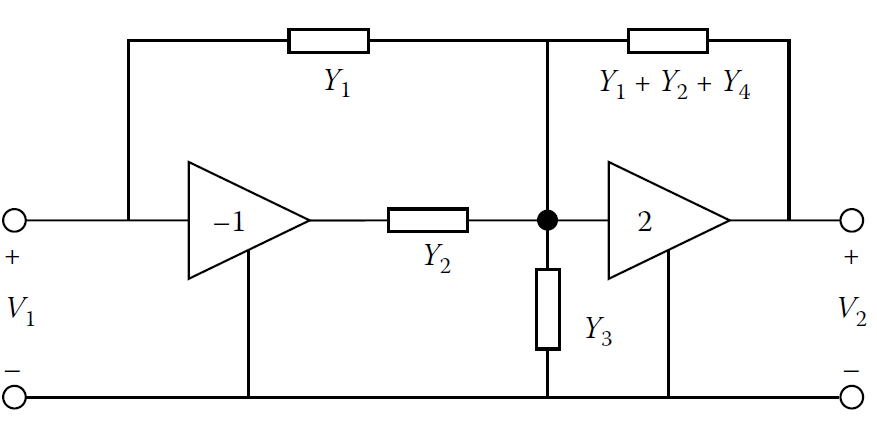
\includegraphics[scale=0.5]{Fig/Q6.png}
            \caption{\label{fig:Q6} Biquad active filter.}
        \end{center}
    \end{figure}
    \begin{figure}[H]
        \begin{center}
            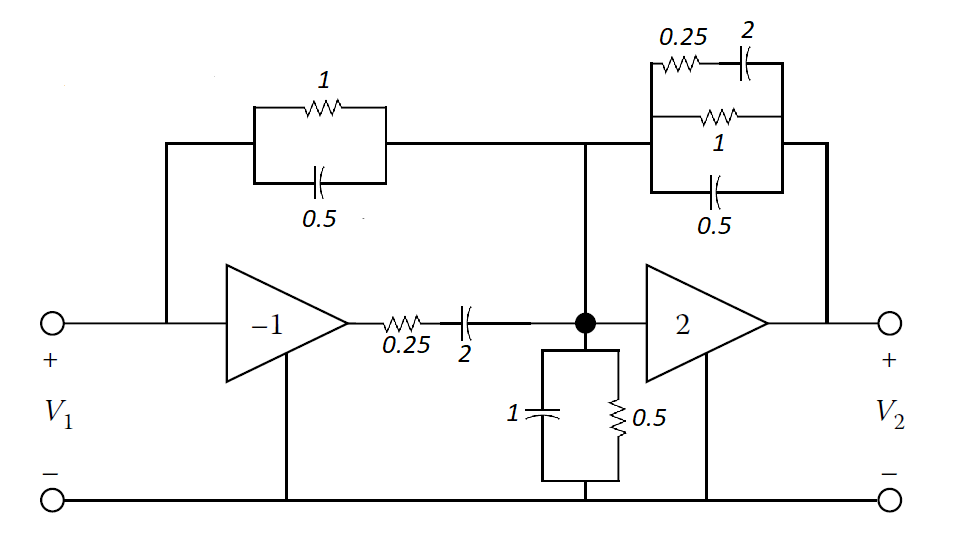
\includegraphics[scale=0.5]{Fig/Q6_1.png}
            \caption{\label{fig:Q6_1} A sample customized realization of the biquad active filter.}
        \end{center}
    \end{figure}


    %--------------------------------------------
    \begin{subquestion}{Simulate the circuit in PSpice and investigate the filtering response of the circuit for various configurations of $Y_1$, $Y_2$, $Y_3$ and $Y_4$. Especially, demonstrate how the biquad filter can have lowpass, highpass, bandpass, and bandstop frequency responses.}
        \answer{
            \begin{figure}[H]
                \begin{center}
                    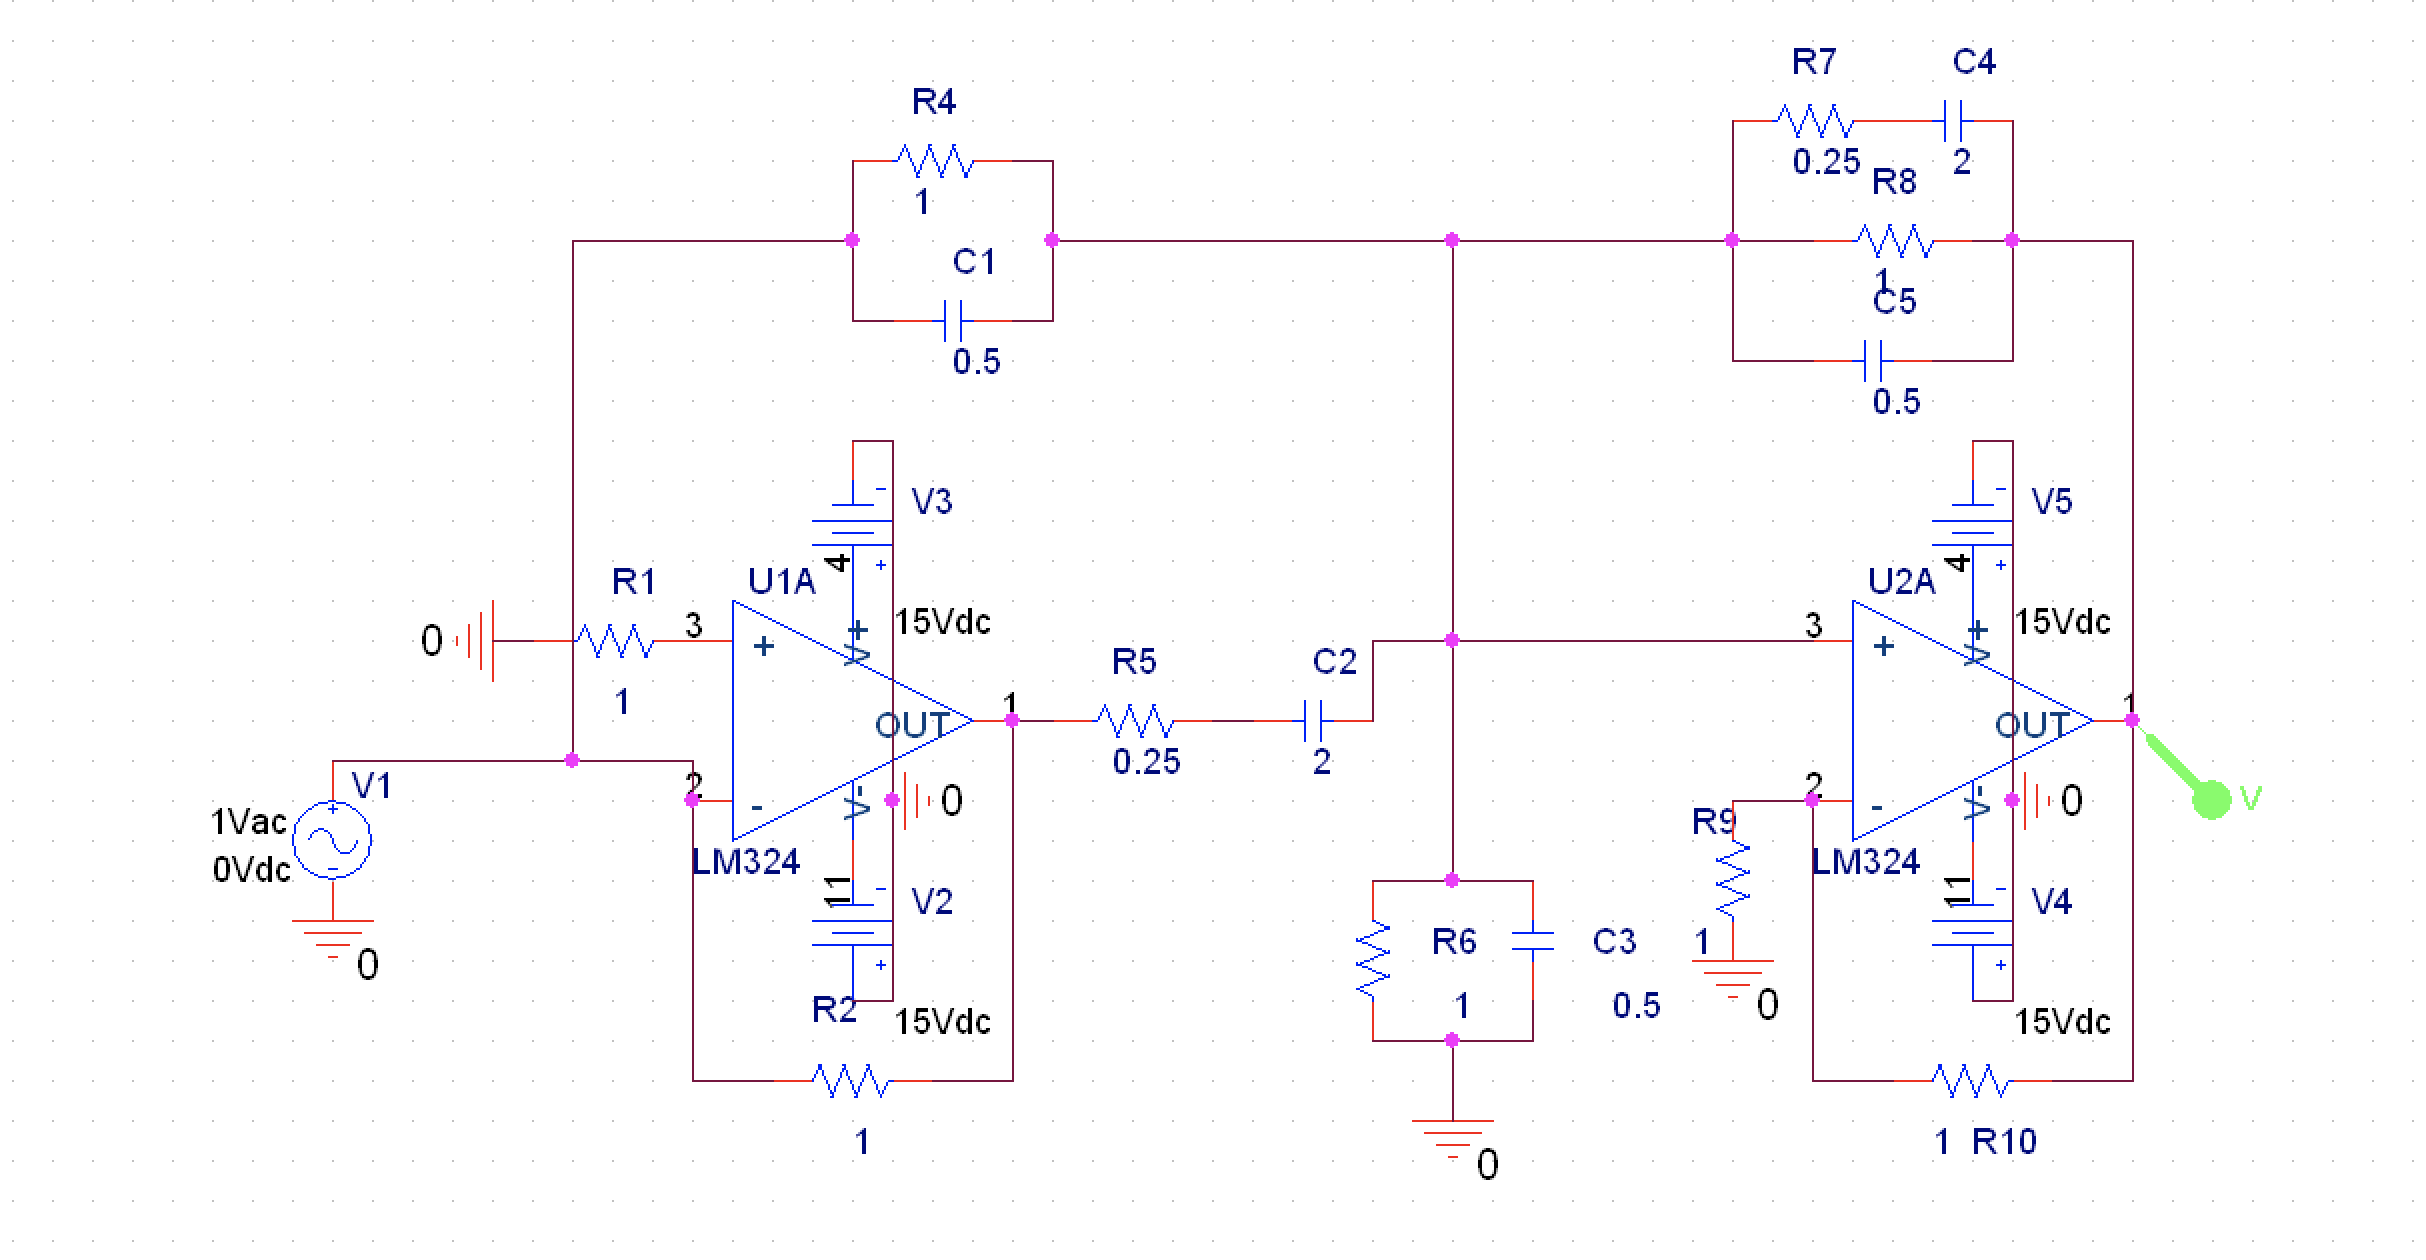
\includegraphics[scale=0.3]{Fig/Q6aa.png}
                    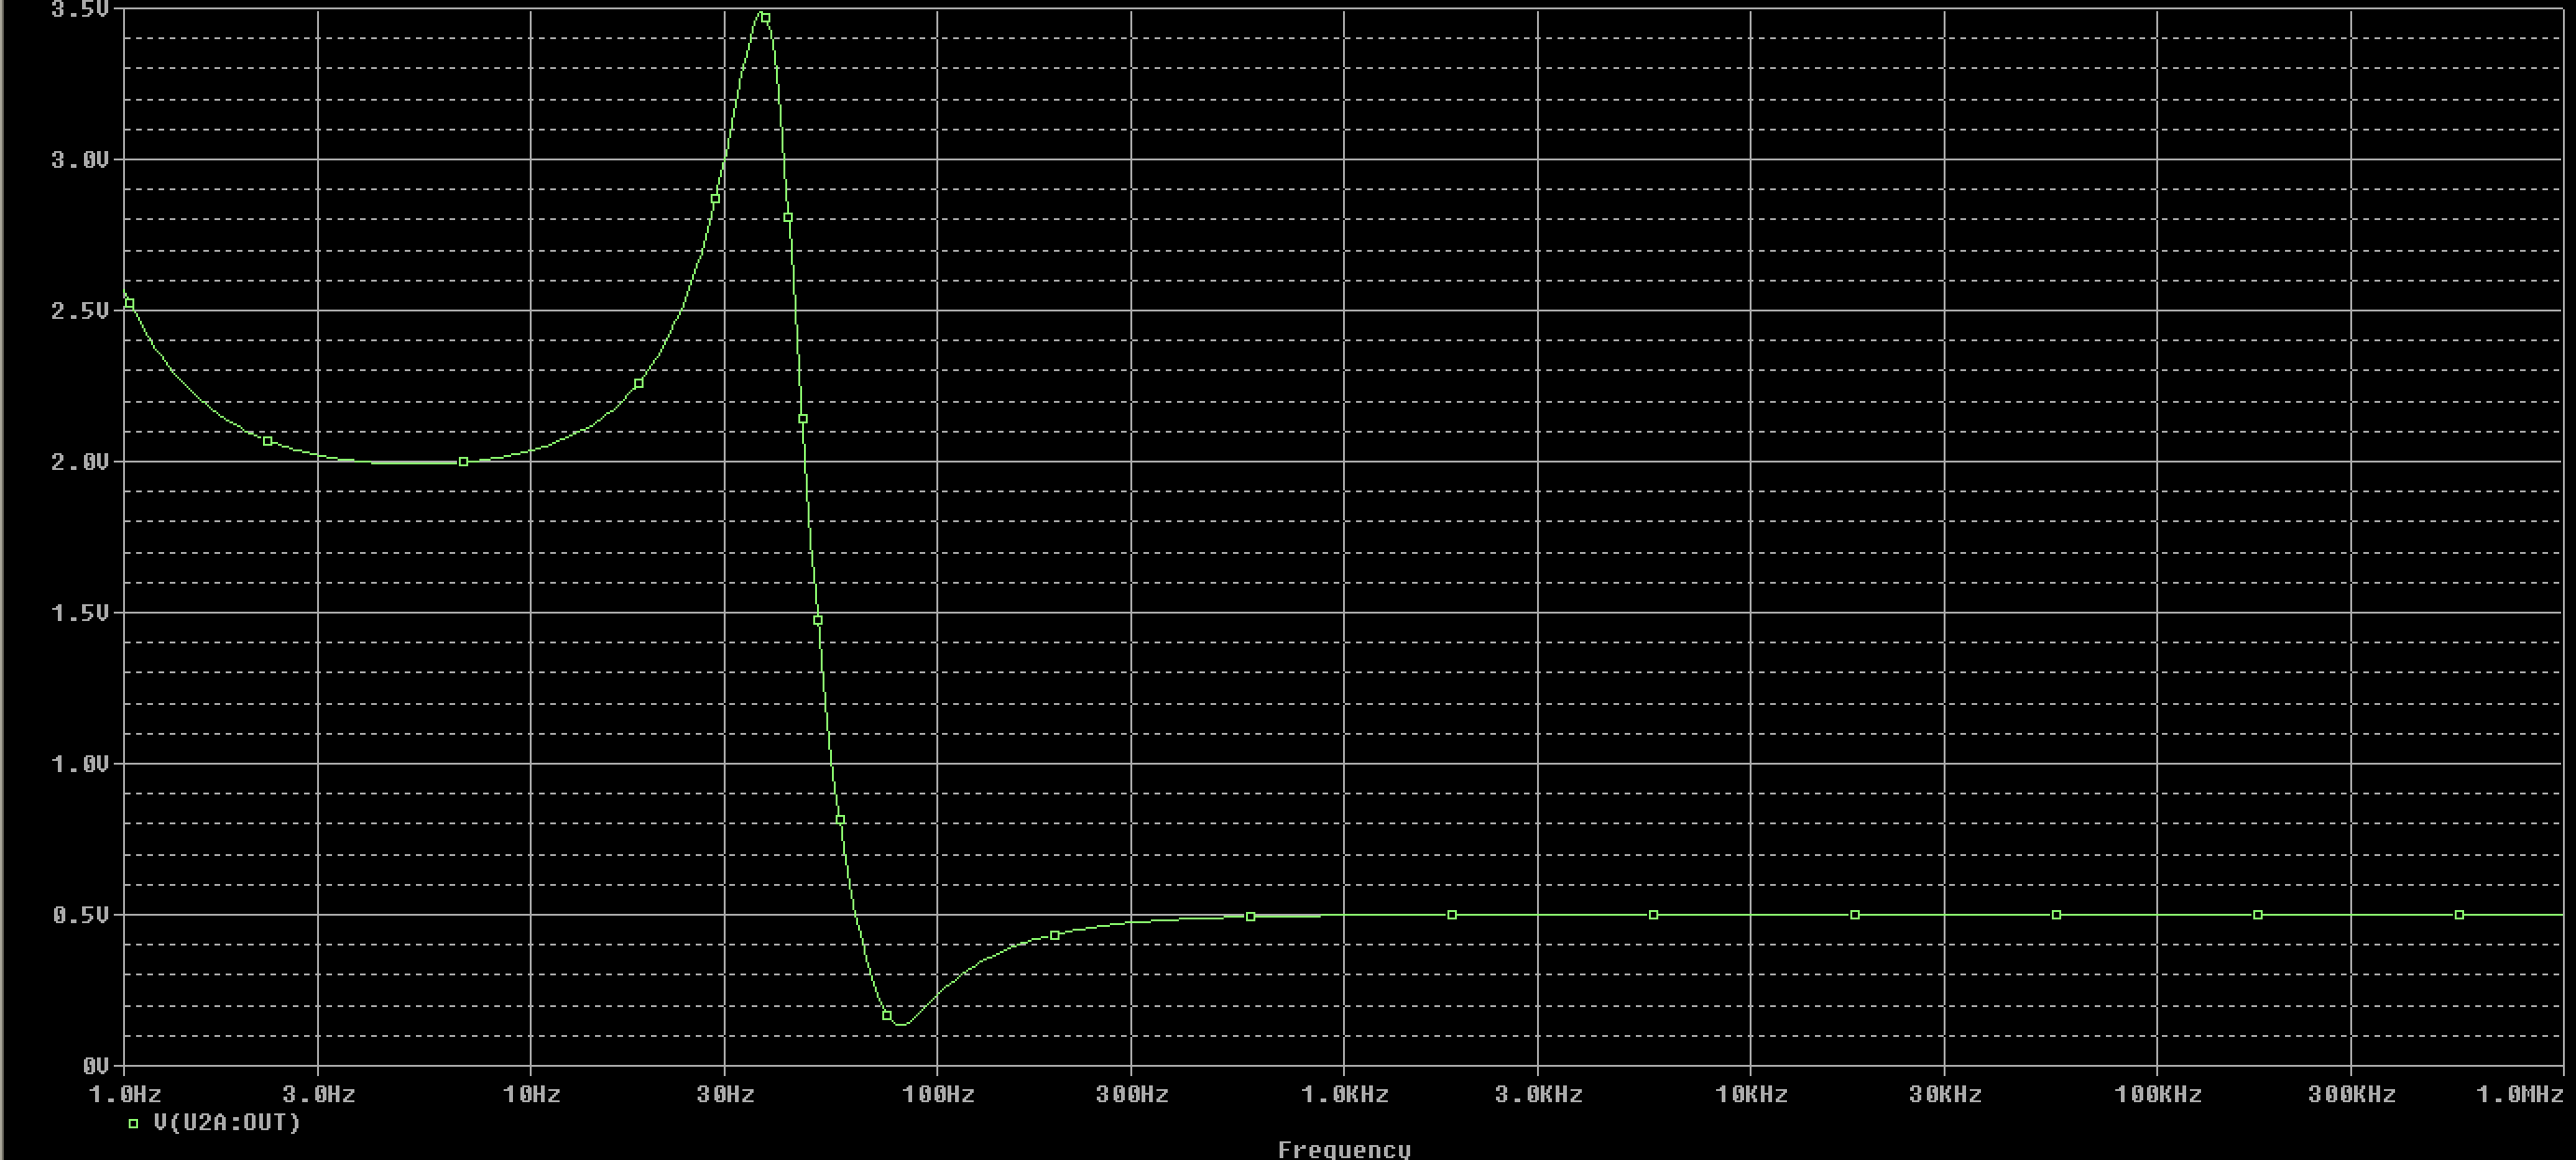
\includegraphics[scale=0.25]{Fig/Q6ab.png}
                    \caption{A bandpass filter designed using biquad filter.}
                \end{center}
            \end{figure}
            \begin{figure}[H]
                \begin{center}
                    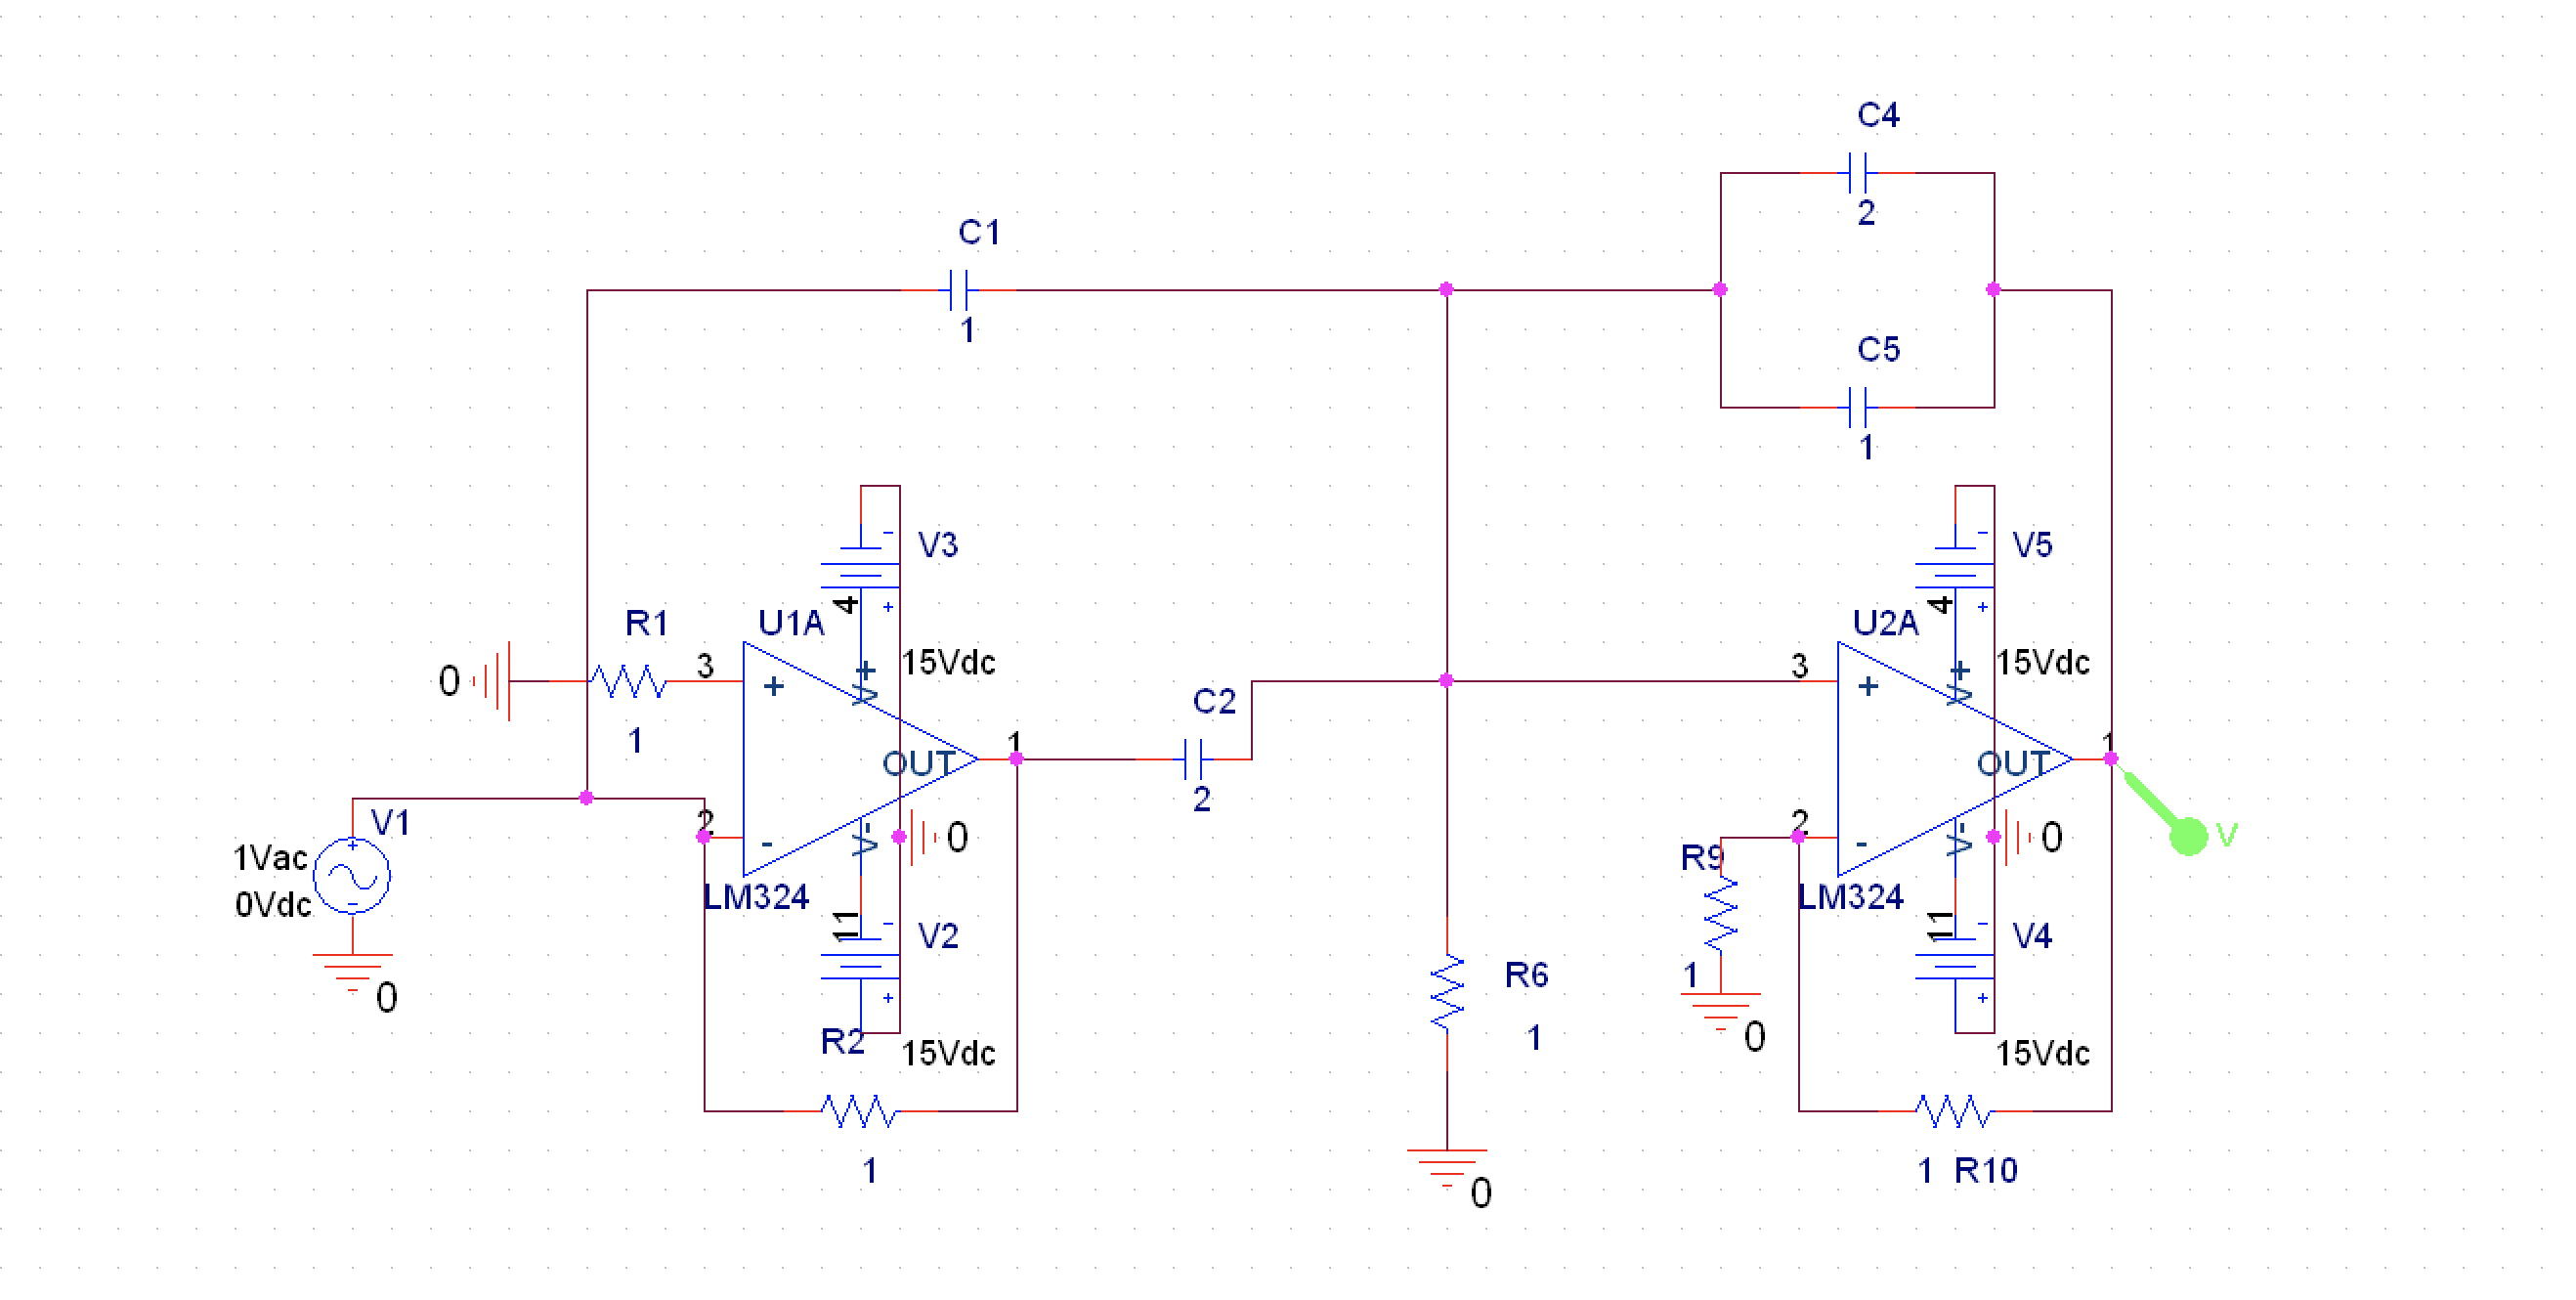
\includegraphics[scale=0.3]{Fig/Q6ba.png}
                    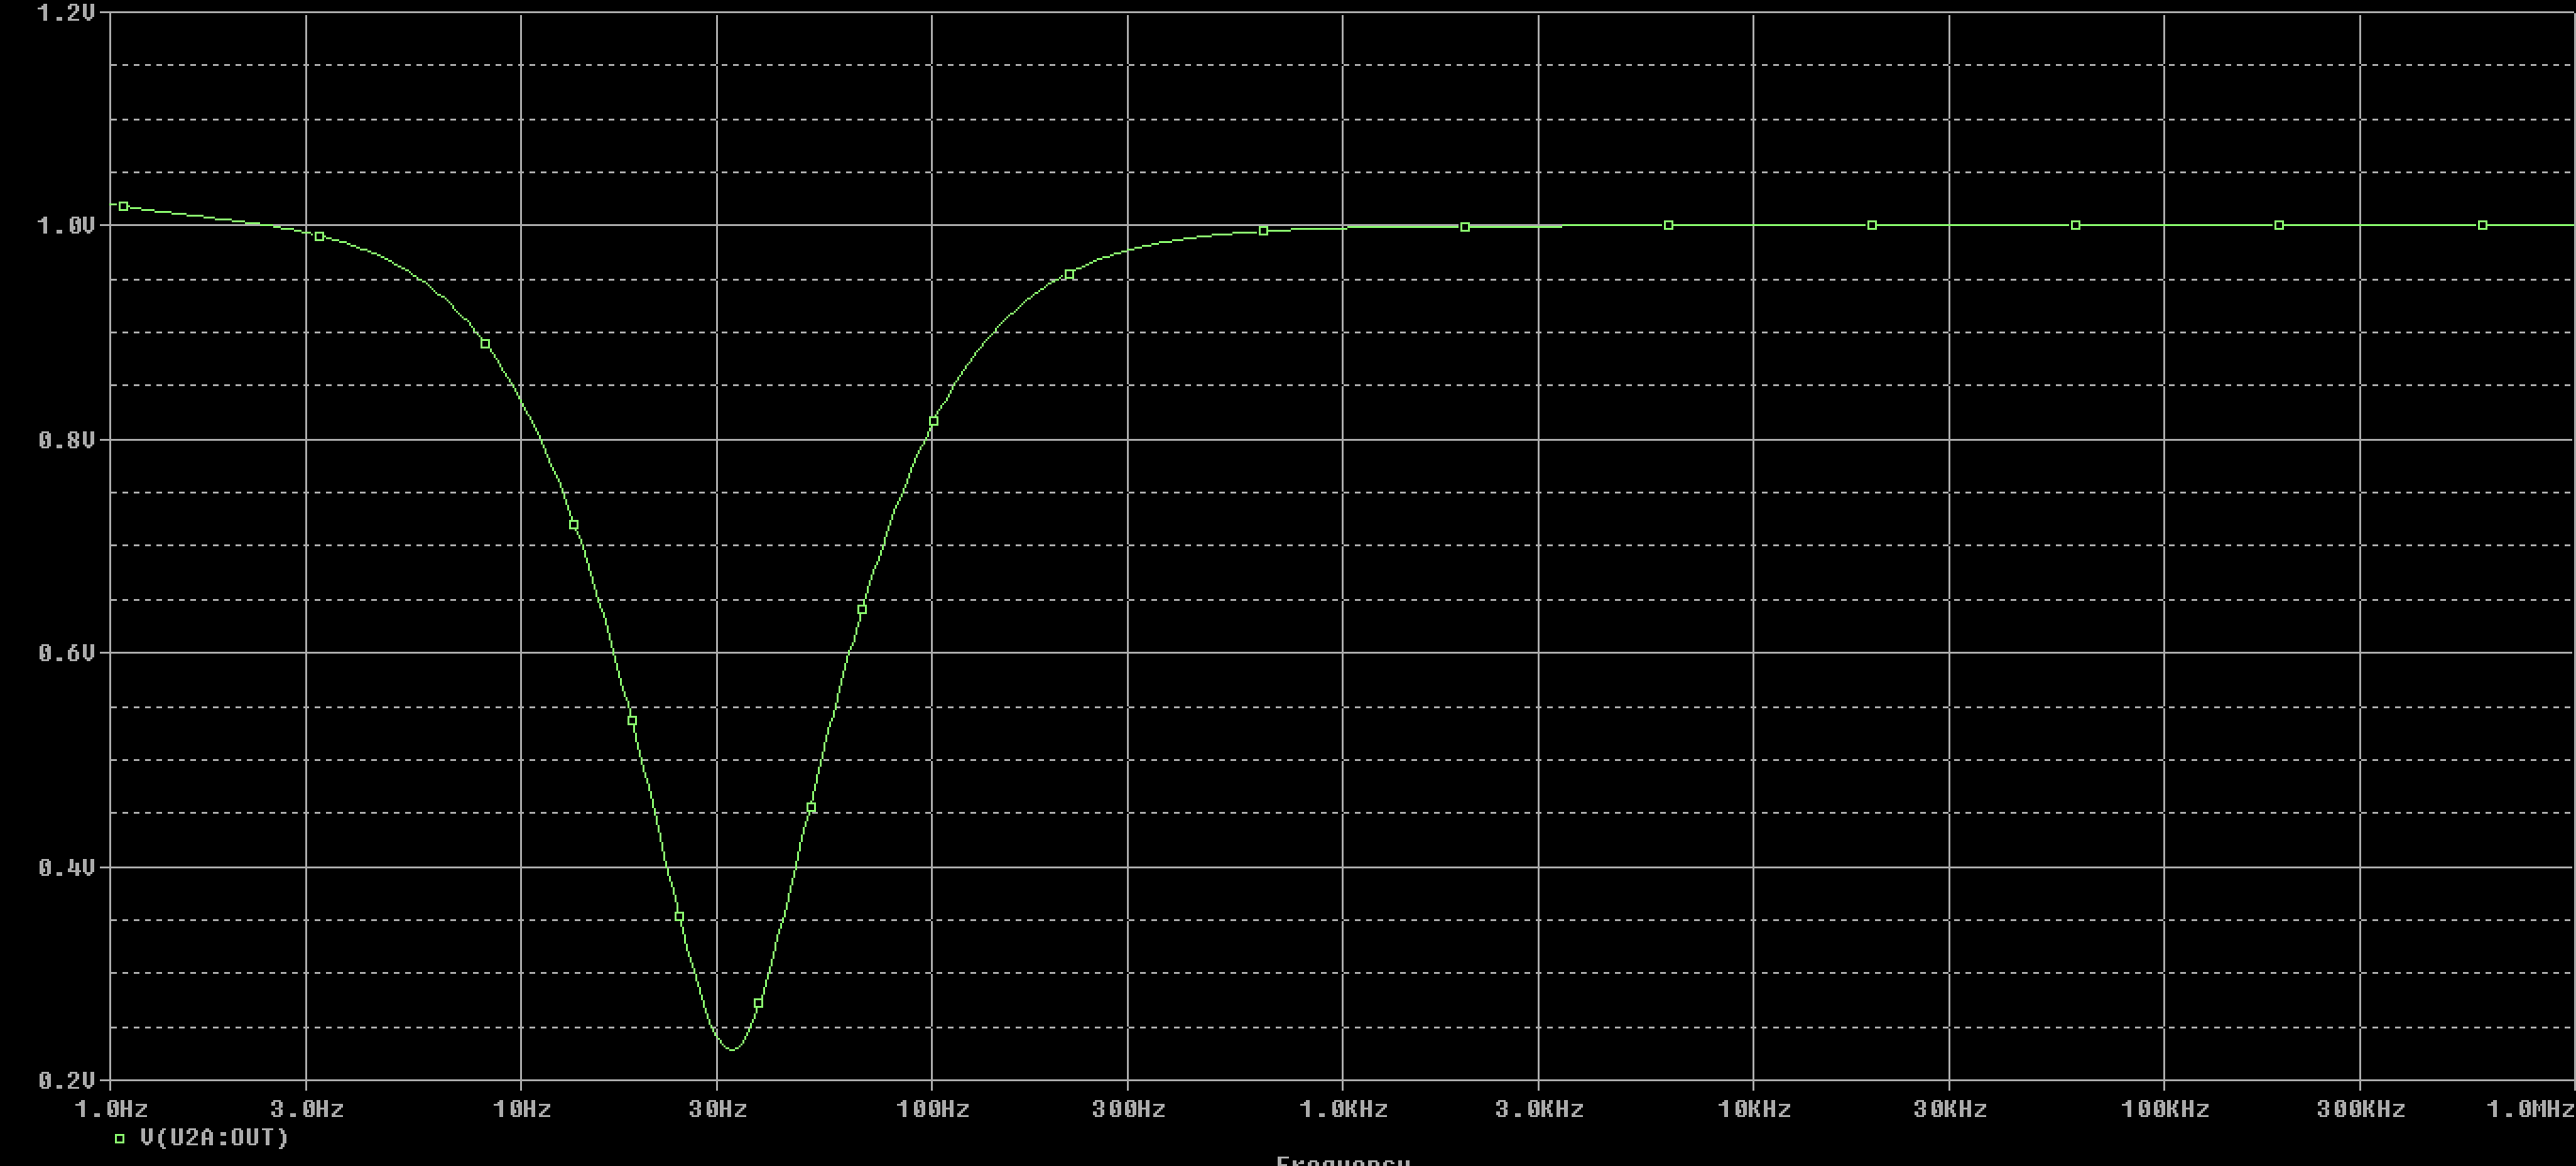
\includegraphics[scale=0.25]{Fig/Q6bb.png}
                    \caption{A bandstop filter designed using biquad filter.}
                \end{center}
            \end{figure}
            \begin{figure}[H]
                \begin{center}
                    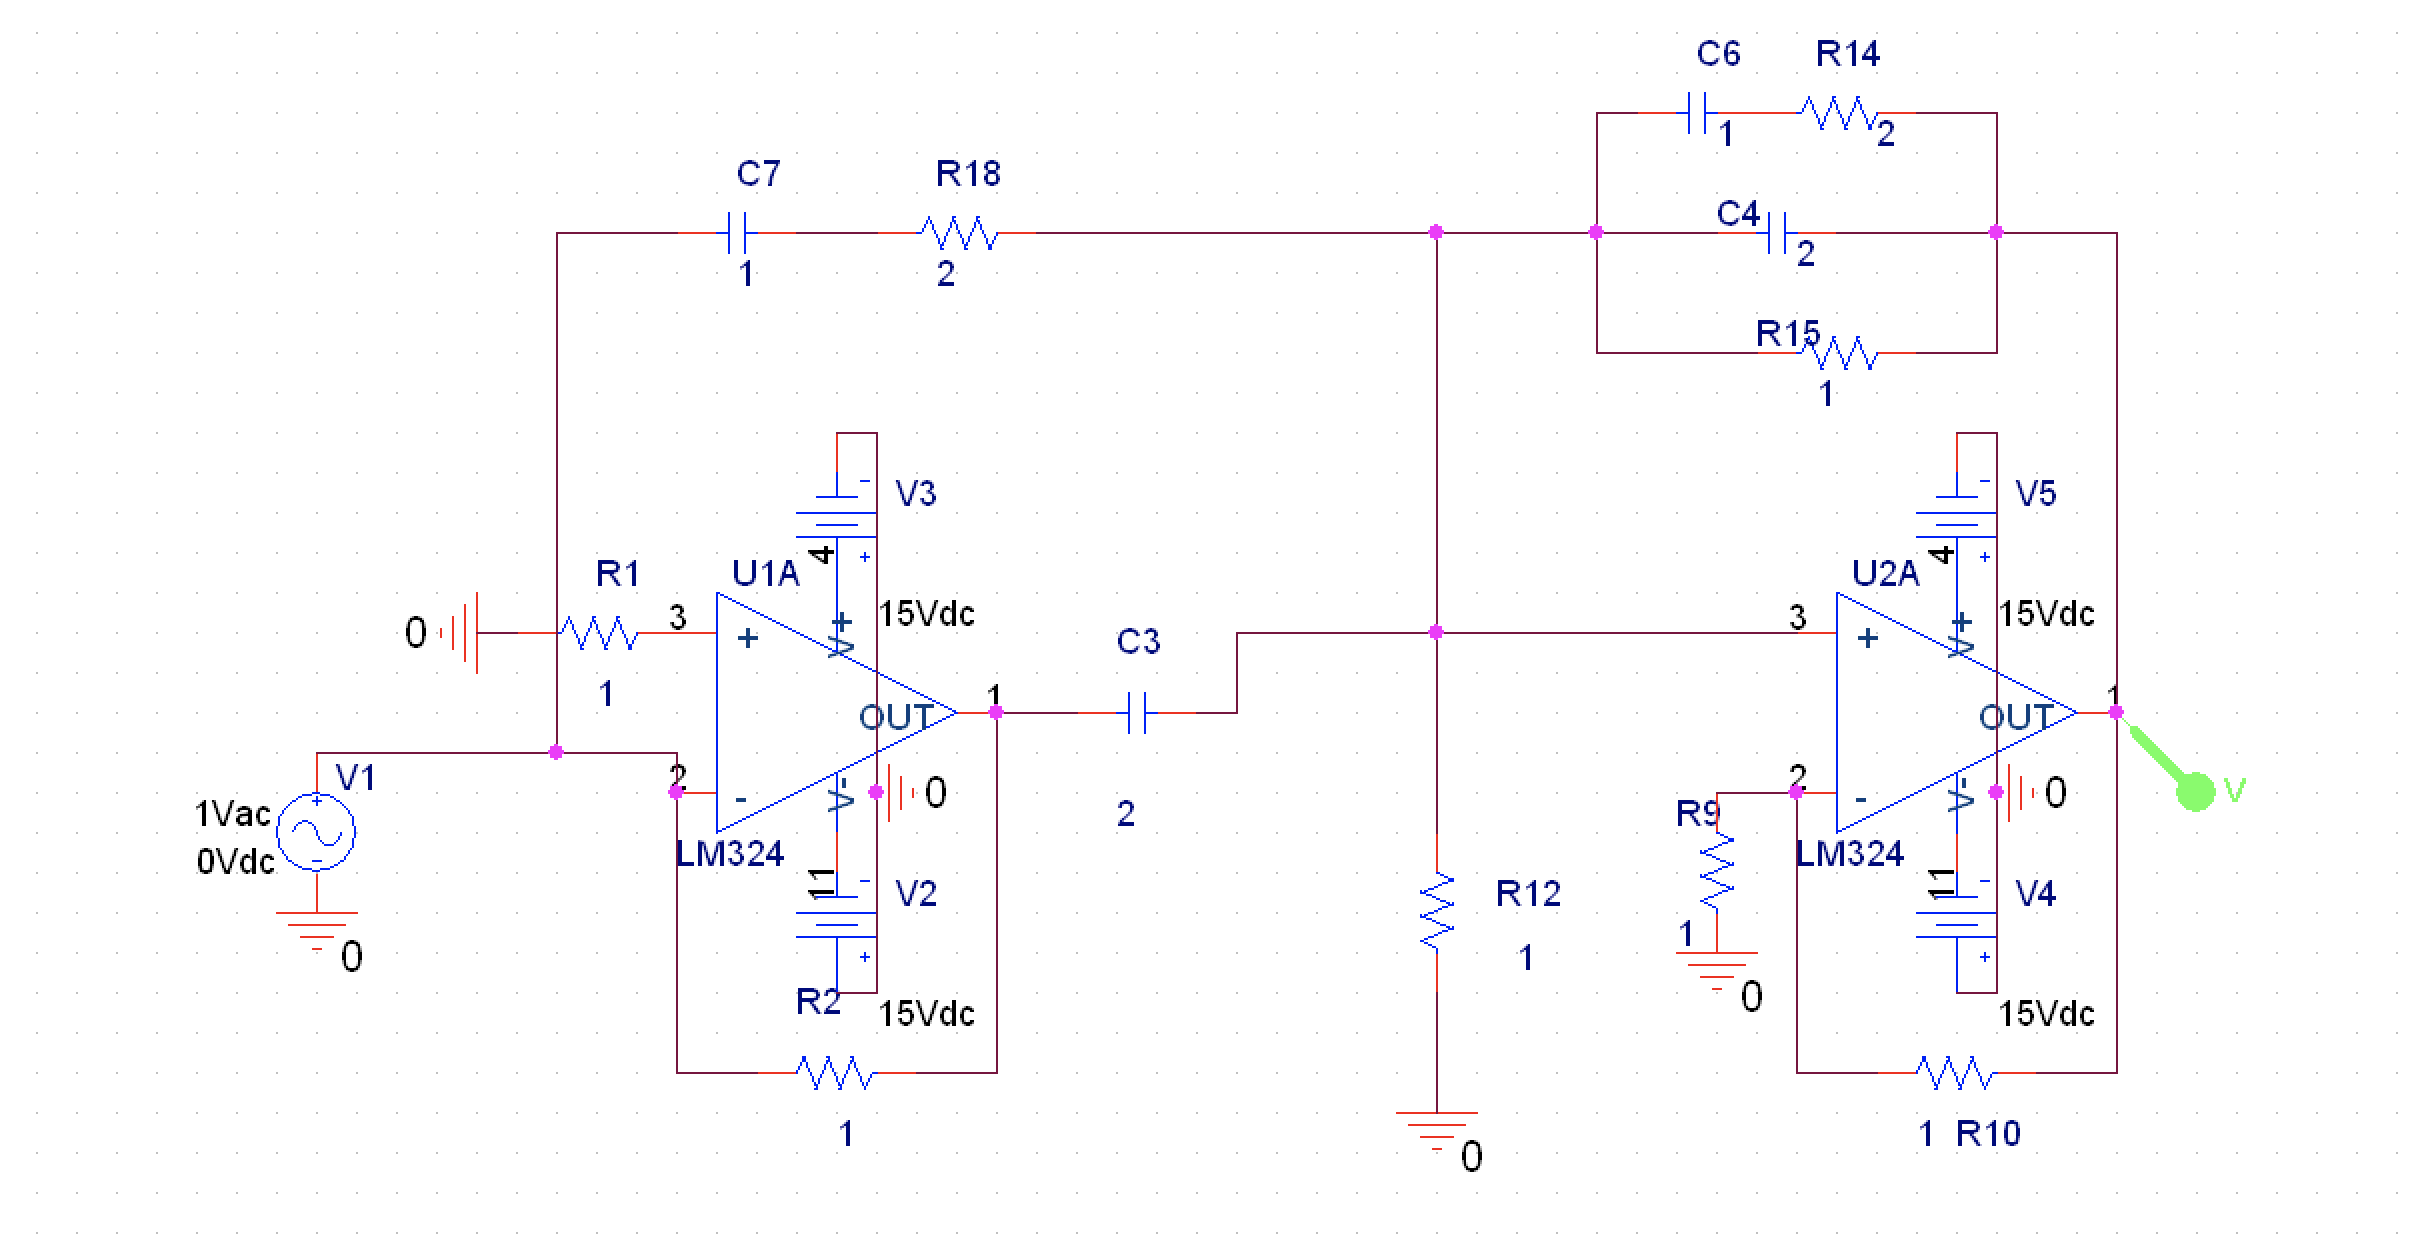
\includegraphics[scale=0.3]{Fig/Q6ca.png}
                    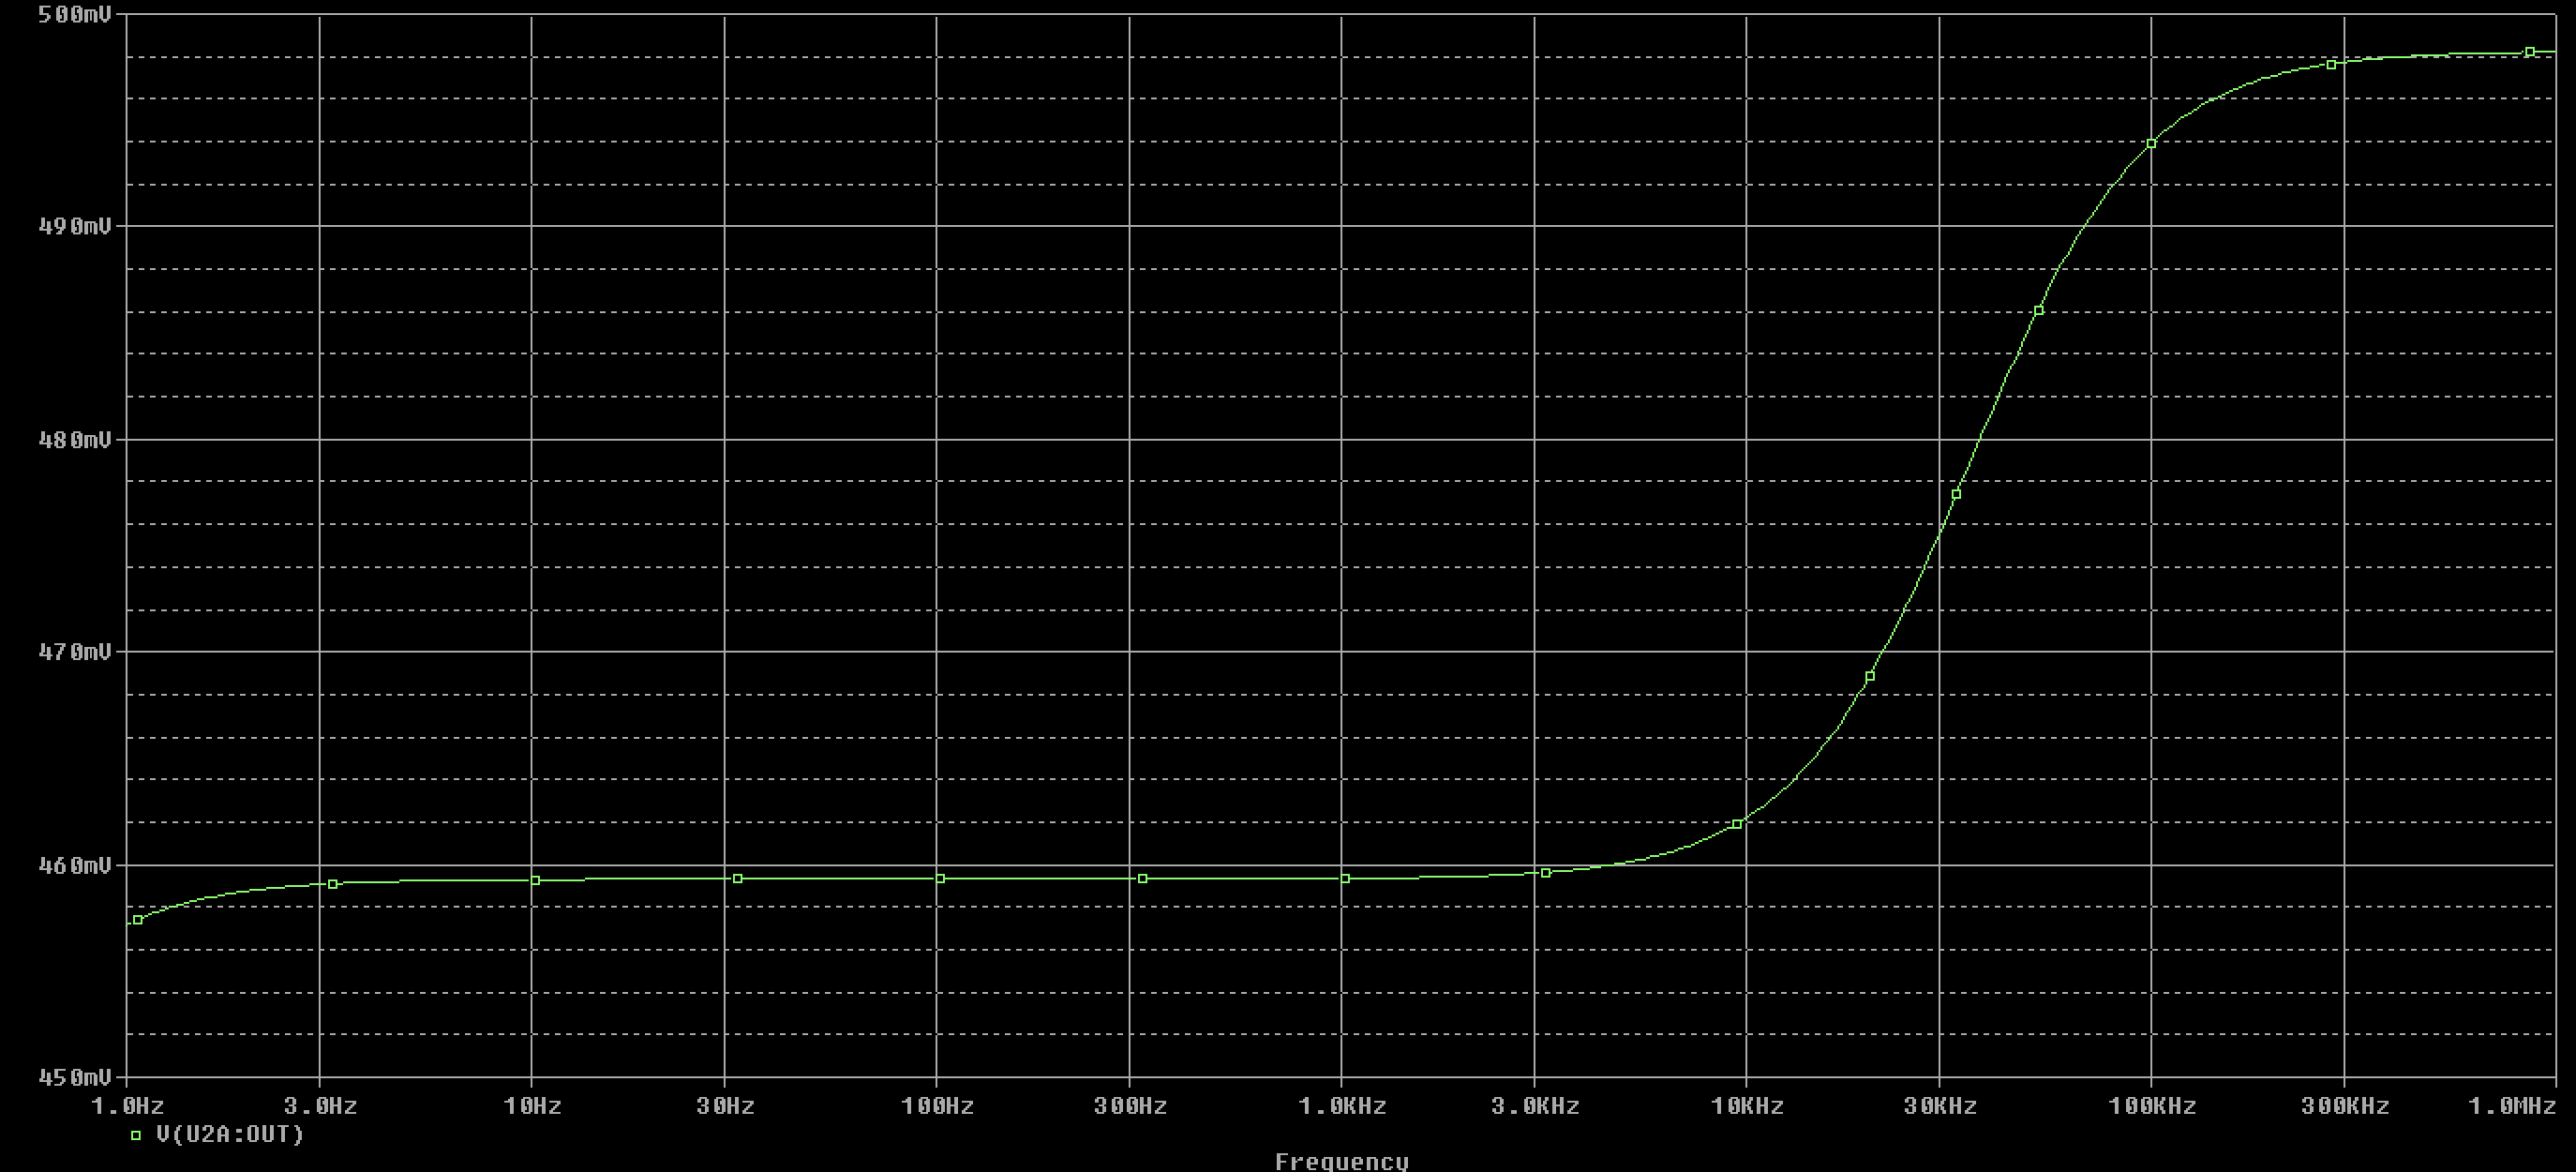
\includegraphics[scale=0.25]{Fig/Q6cb.png}
                    \caption{A highpass filter designed using biquad filter.}
                \end{center}
            \end{figure}
            \begin{figure}[H]
                \begin{center}
                    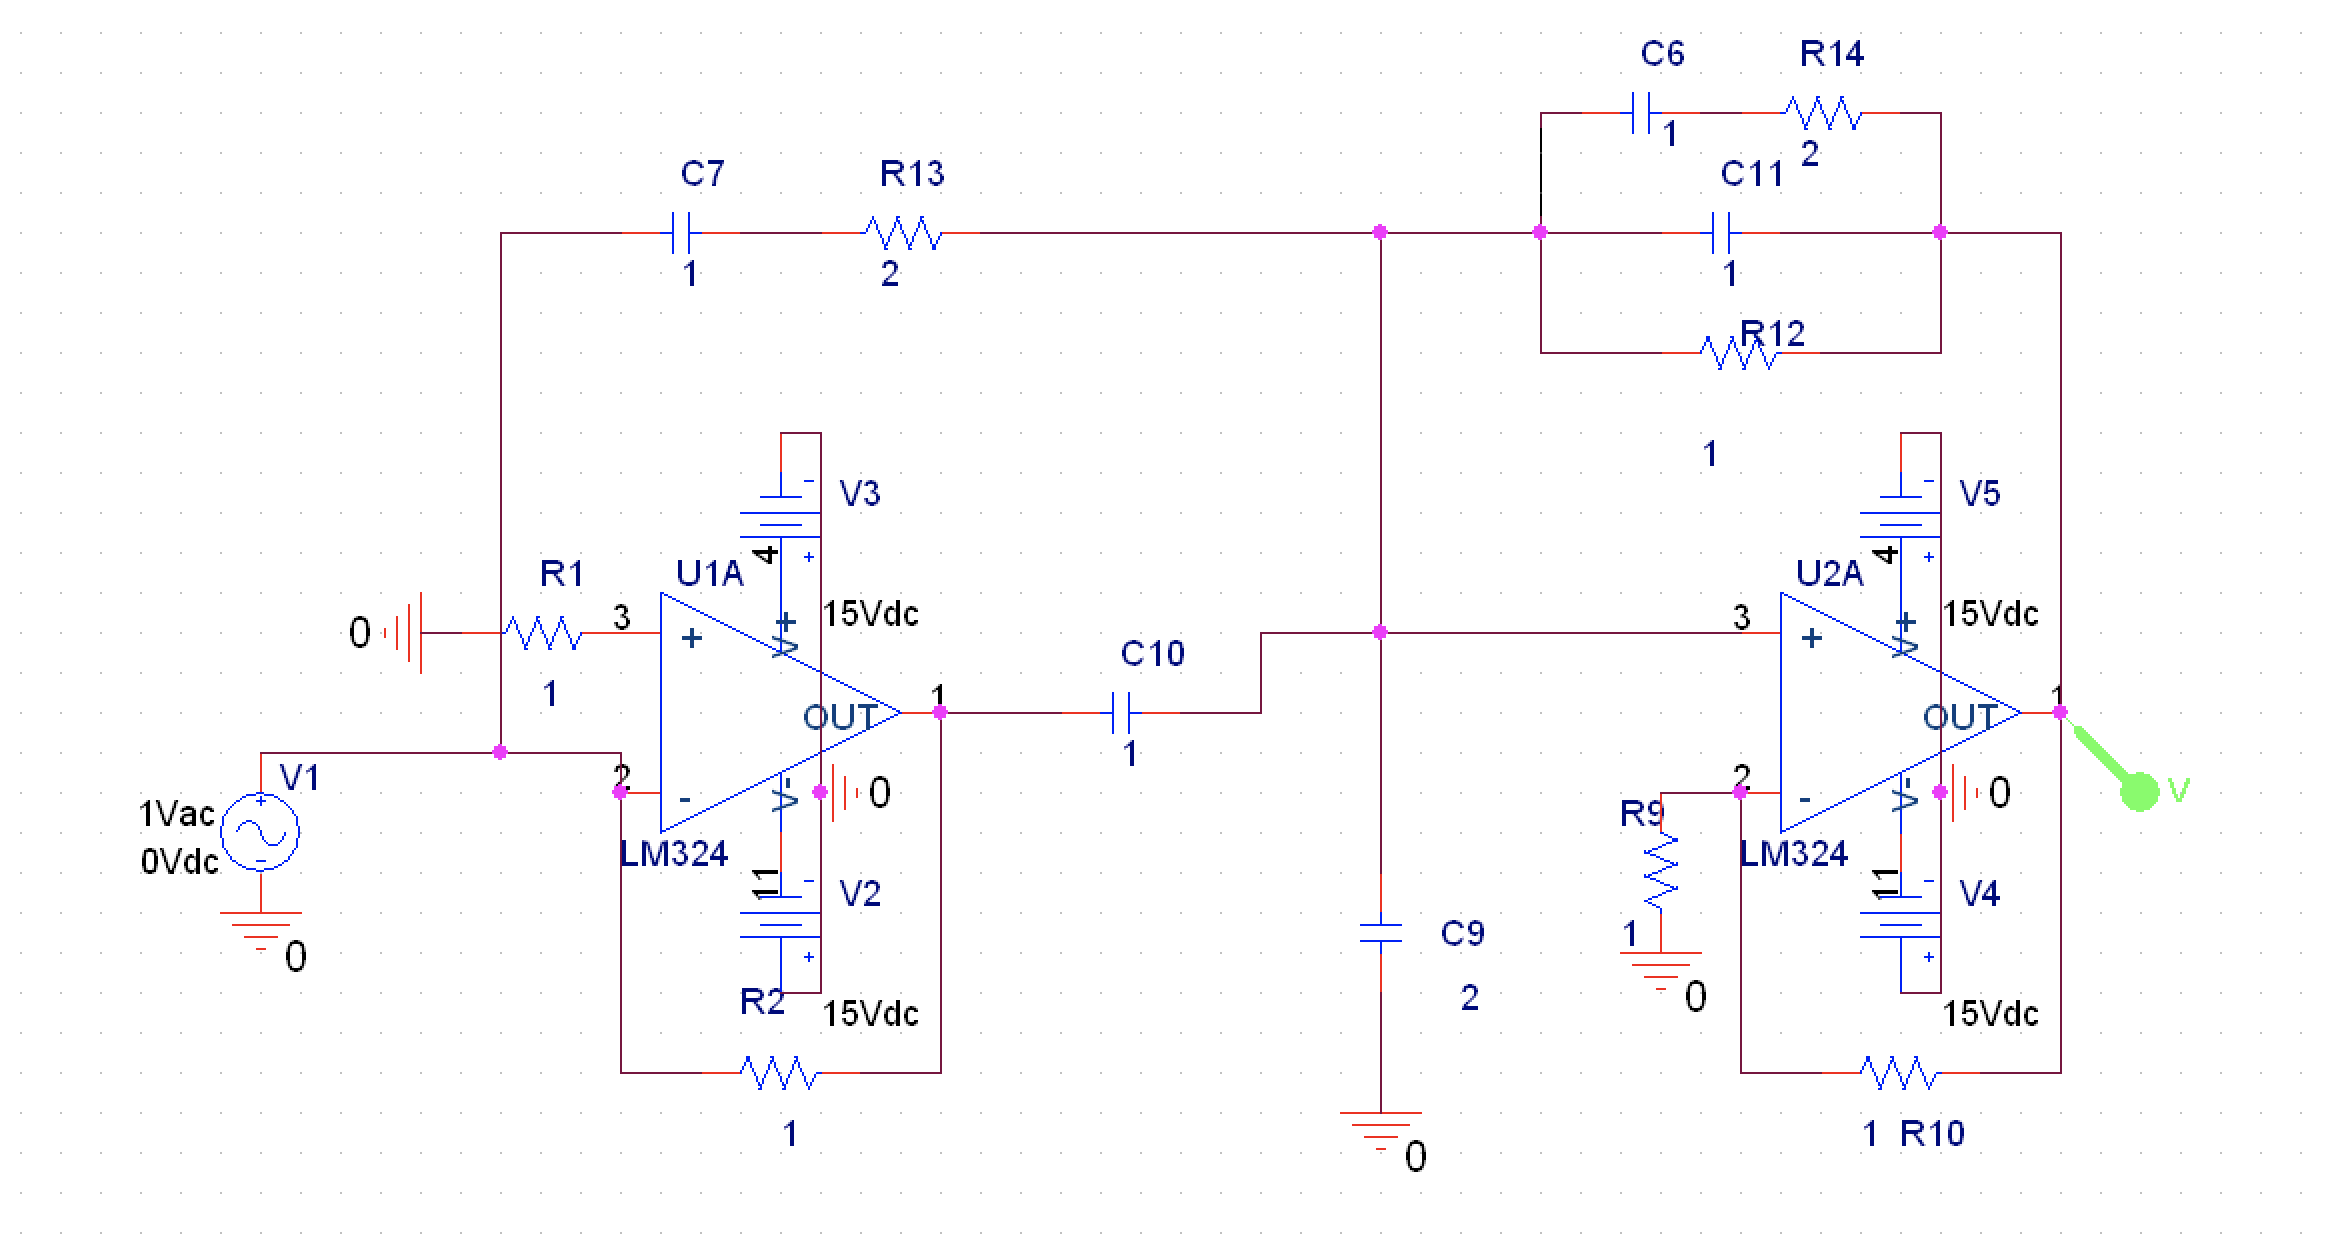
\includegraphics[scale=0.3]{Fig/Q6da.png}
                    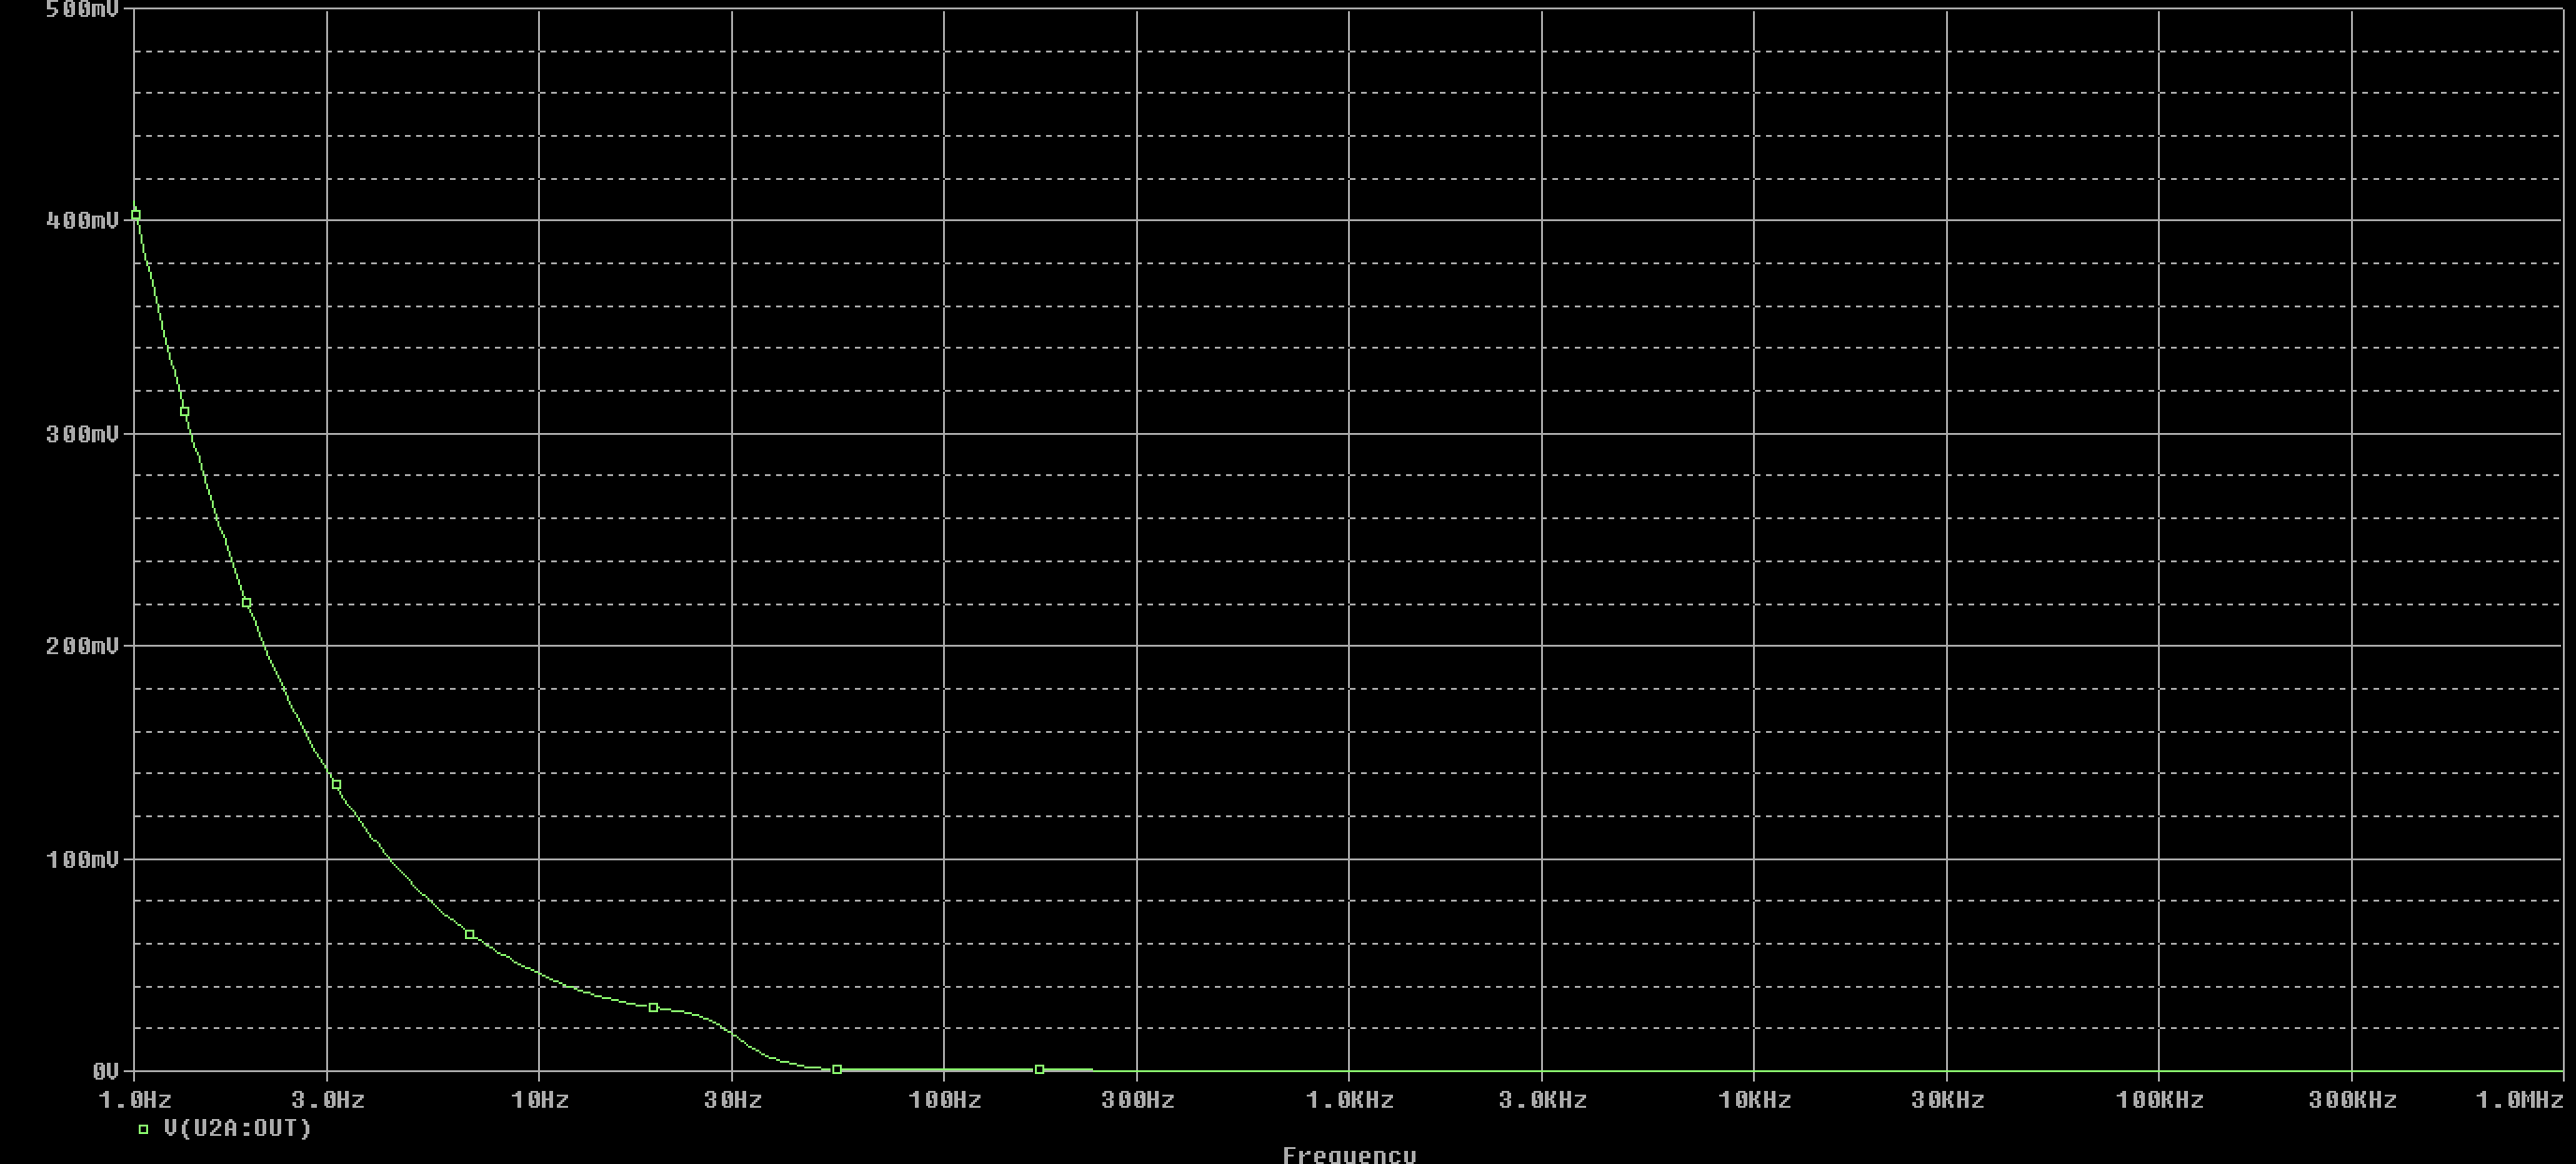
\includegraphics[scale=0.25]{Fig/Q6db.png}
                    \caption{A lowpass filter designed using biquad filter.}
                \end{center}
            \end{figure}
        }
    \end{subquestion}
    %--------------------------------------------
    \begin{subquestion}{What is an all-pass filter and how can it be implemented using a biquad?}
        \answer{
            An all-pass filter is a type of filter that passes all frequencies with unity gain, but changes the phase relationship between different frequencies.
            \begin{figure}[H]
                \begin{center}
                    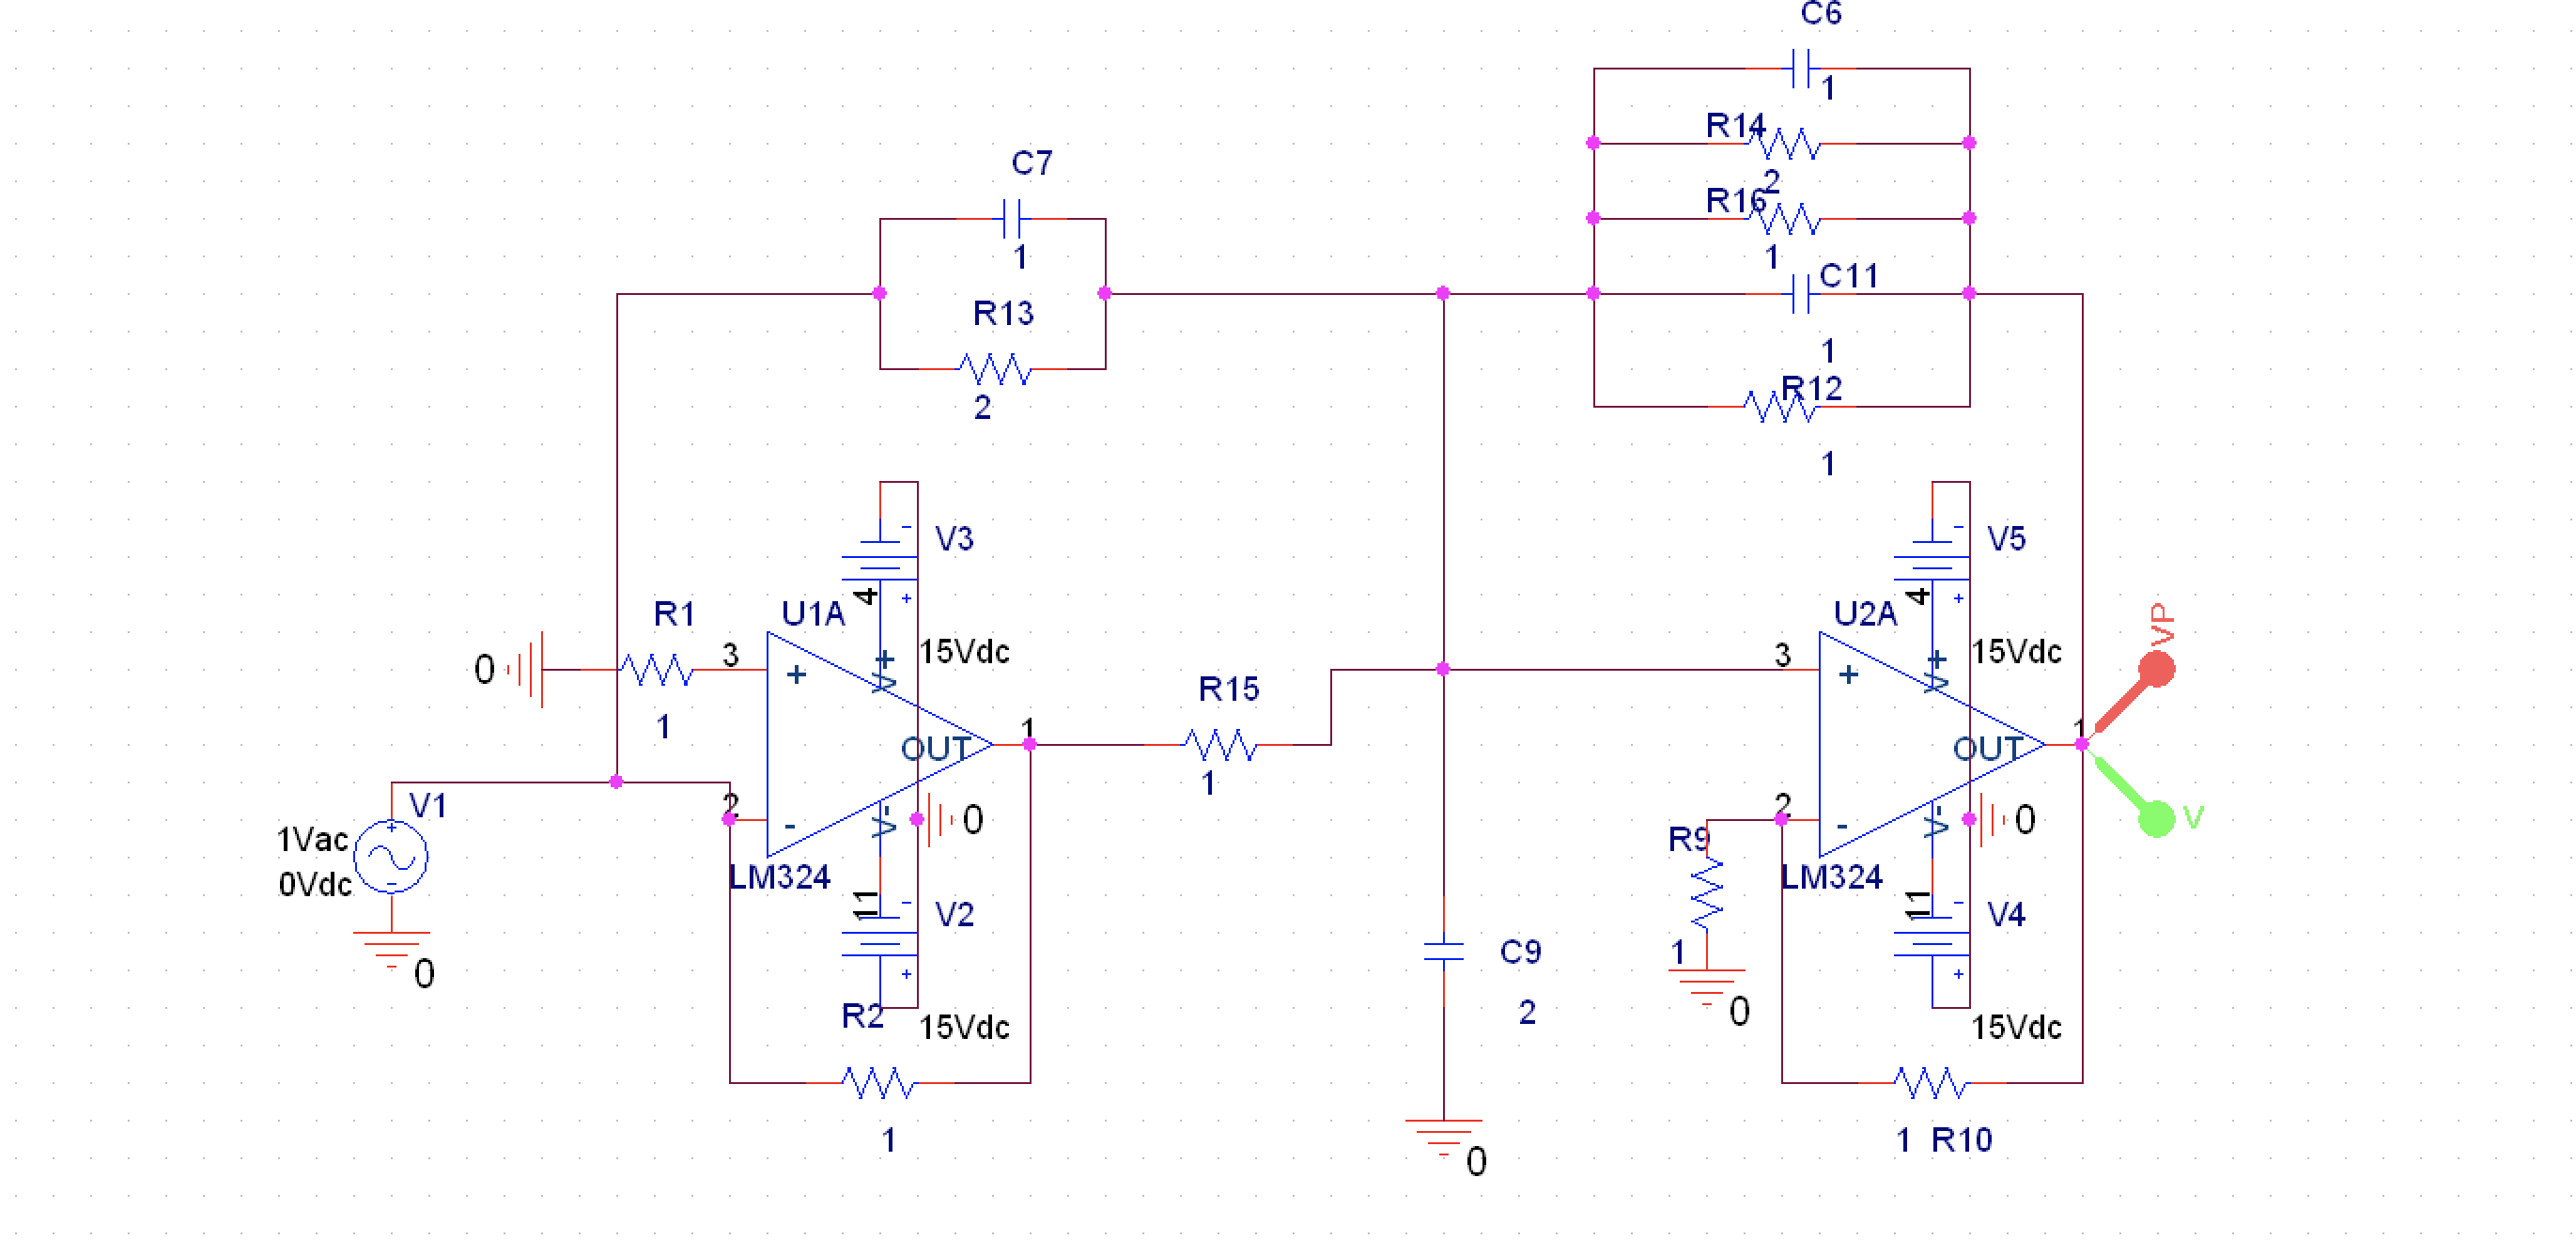
\includegraphics[scale=0.3]{Fig/Q6za.png}
                    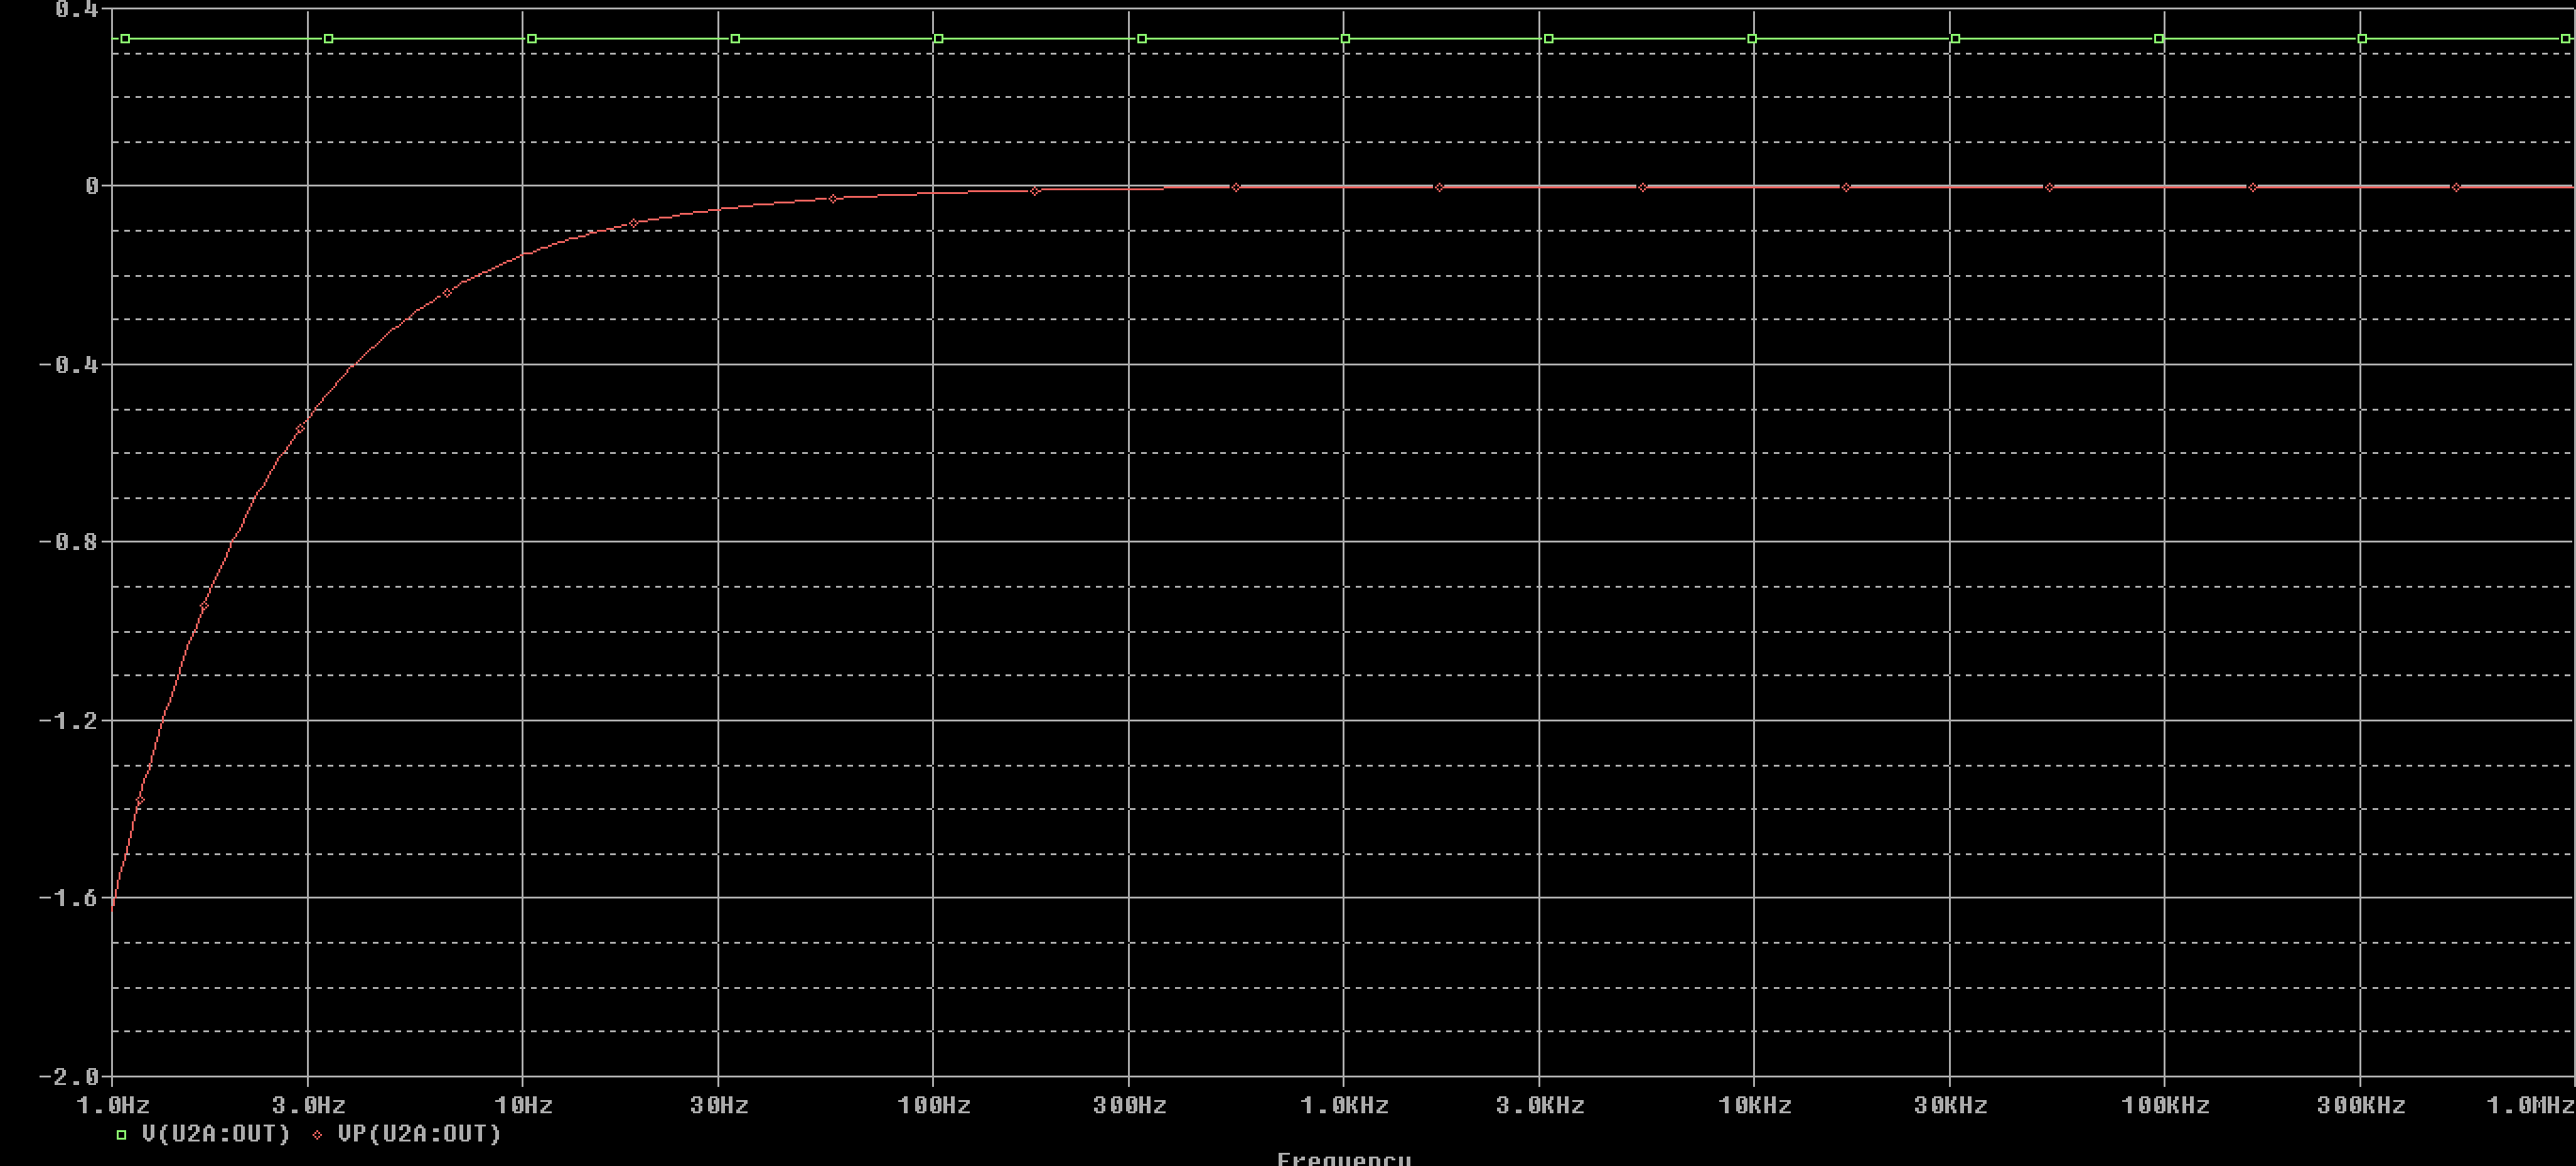
\includegraphics[scale=0.25]{Fig/Q6zb.png}
                    \caption{A all-pass filter designed using biquad filter.}
                \end{center}
            \end{figure}
        }
    \end{subquestion}

\end{question}


%----------------------------------------------------------------------------------------
%	QUESTION 7
%----------------------------------------------------------------------------------------

\begin{question}

    \questiontext{Return your work report by filling the \LaTeX template of the manual. Include useful and high-quality images to make the report more readable and understandable.}

\end{question}

%----------------------------------------------------------------------------------------

\end{document}
